%%
%%  results.tex - Obstacle Detection and Planning for Autonomous Vehicles based on Computer Vision Techniques
%%
%%  Copyright 2014 Néstor Morales <nestor@isaatc.ull.es>
%%
%%  This work is licensed under a Creative Commons Attribution 4.0 International License.
%%


\chapter{Results}\label{ch:chapter08}

In this chapter, we will show the results obtained for each of the methods described in the previous chapters. Each section corresponds to one method. At the end of this chapter, we will try to put all the definitive methods together and, in the last chapter, the conclusions obtained in this thesis are summarized.

\graphicspath{{./images/chapter01/bmps/}{./images/chapter01/vects/}{./images/chapter01/}}
\section{Change detection for obstacle localization in images}\label{ch:chapter01_02}

In order to know the behavior of this method, some tests have been performed. In the following sections the results obtained are introduced.

\subsection{Image registration}\label{ch:chapter01_02_01}

For the analysis of the behavior of the algorithm, more than 86,000 image pairs at different resolutions ($800 \times 600$, $640 \times 480$, $320 \times 240$), distances and angle differences, and with diverse zoom and blurring factors applied to them have been tested. From this study a set of charts, shown at figure \ref{fig:cp01_matching_results} were obtained.

\begin{figure*}[t]
        \centering
        \begin{subfigure}[b]{0.45\textwidth}
	    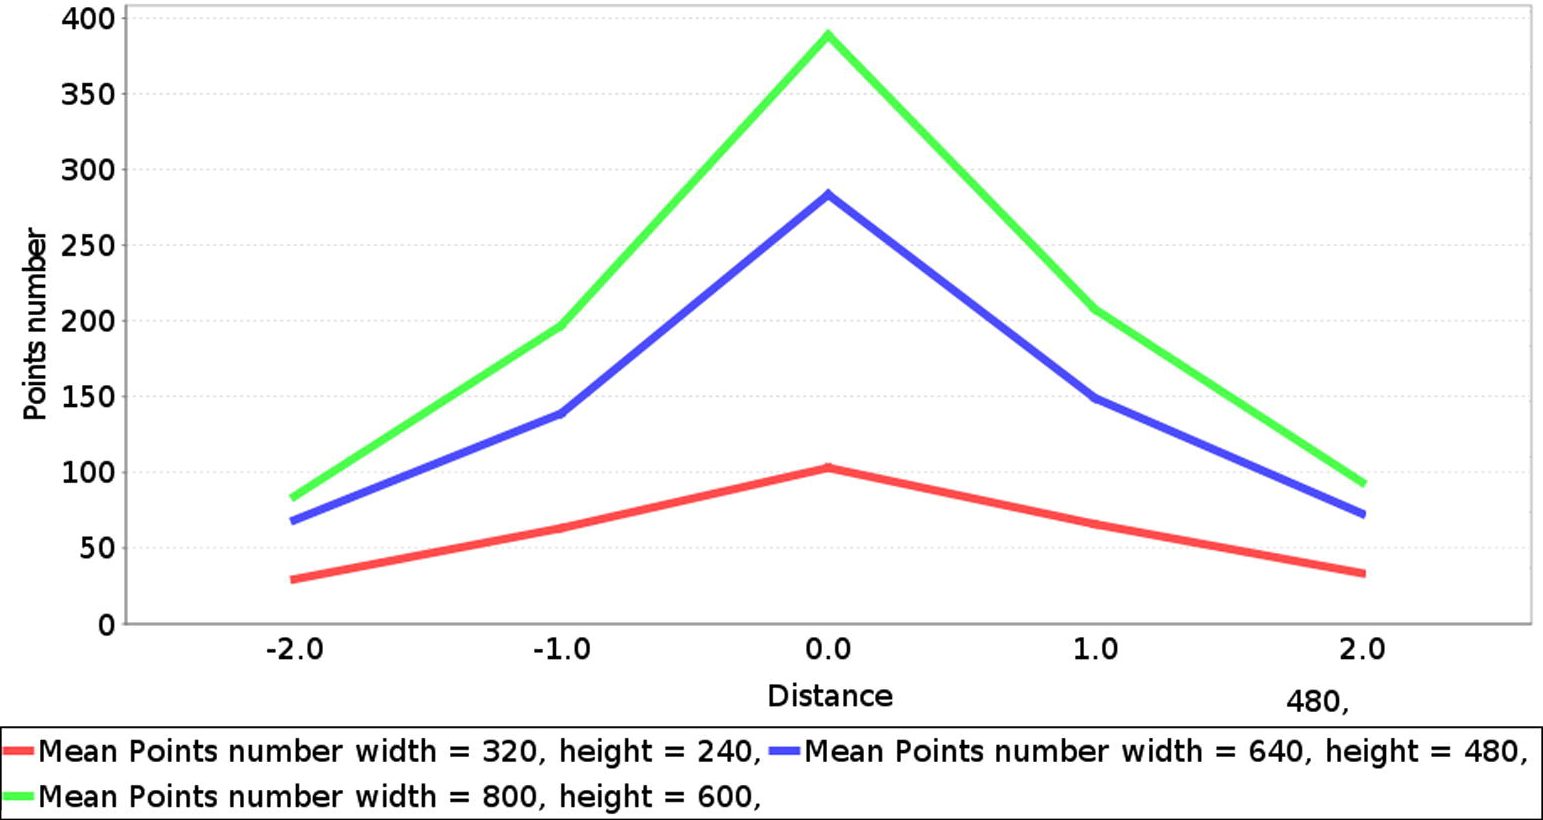
\includegraphics[width=\textwidth]{distVsMatches}
	  \caption{Distance \emph{vs} matched points}\label{fig:cp01_distance_vs_matched}
        \end{subfigure}% 
        ~
        \begin{subfigure}[b]{0.45\textwidth}
	    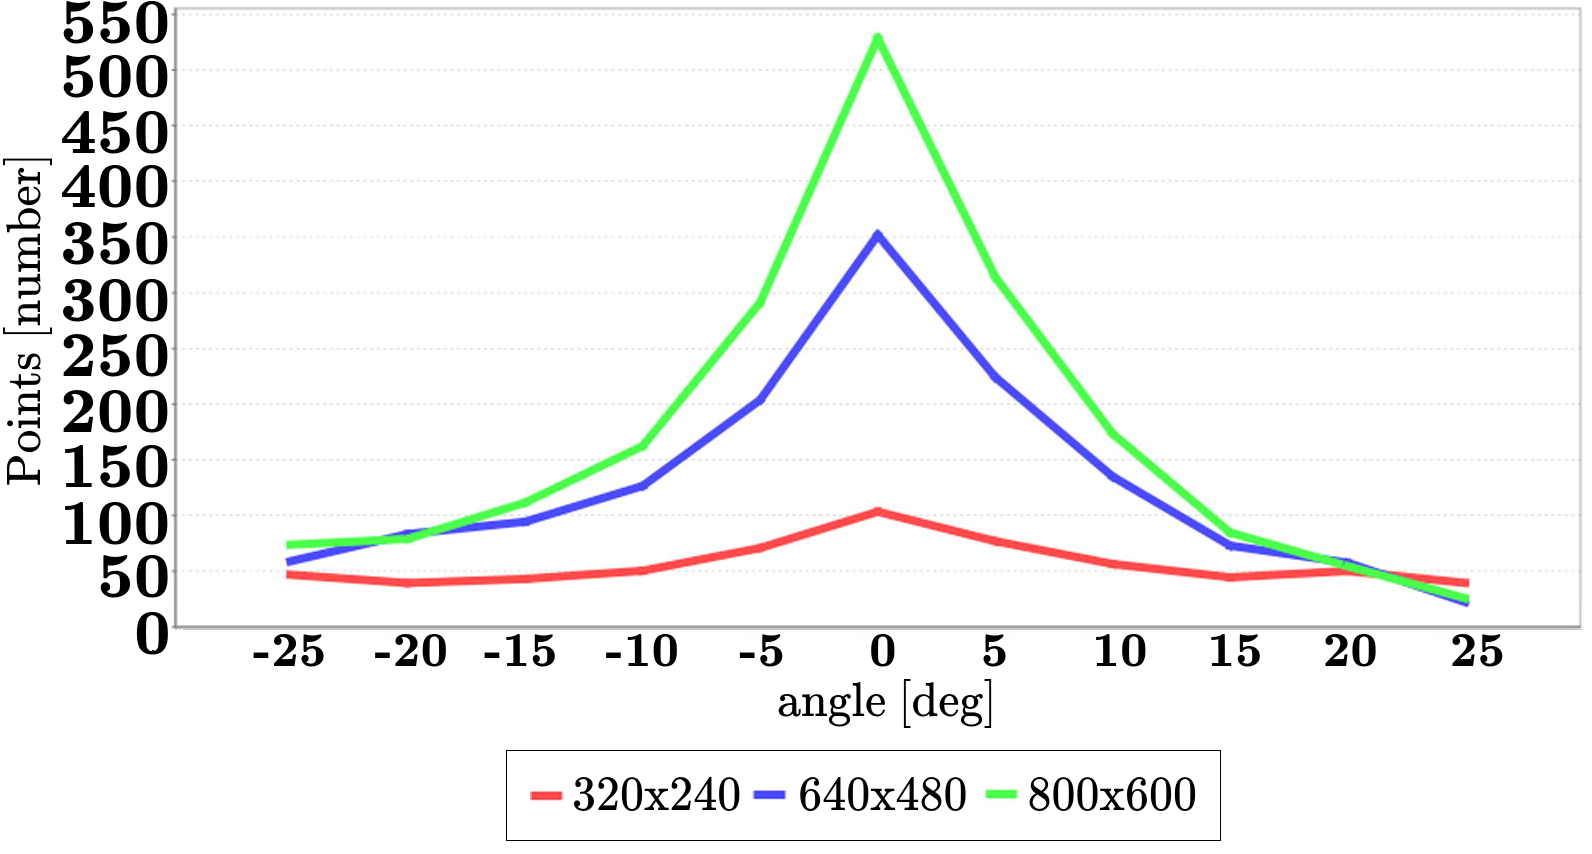
\includegraphics[width=\textwidth]{angleVsMatches}
	  \caption{Angle \emph{vs} matched points}\label{fig:cp01_angle_vs_matched}
        \end{subfigure}%       
        \\
        \begin{subfigure}[b]{0.45\textwidth}
	    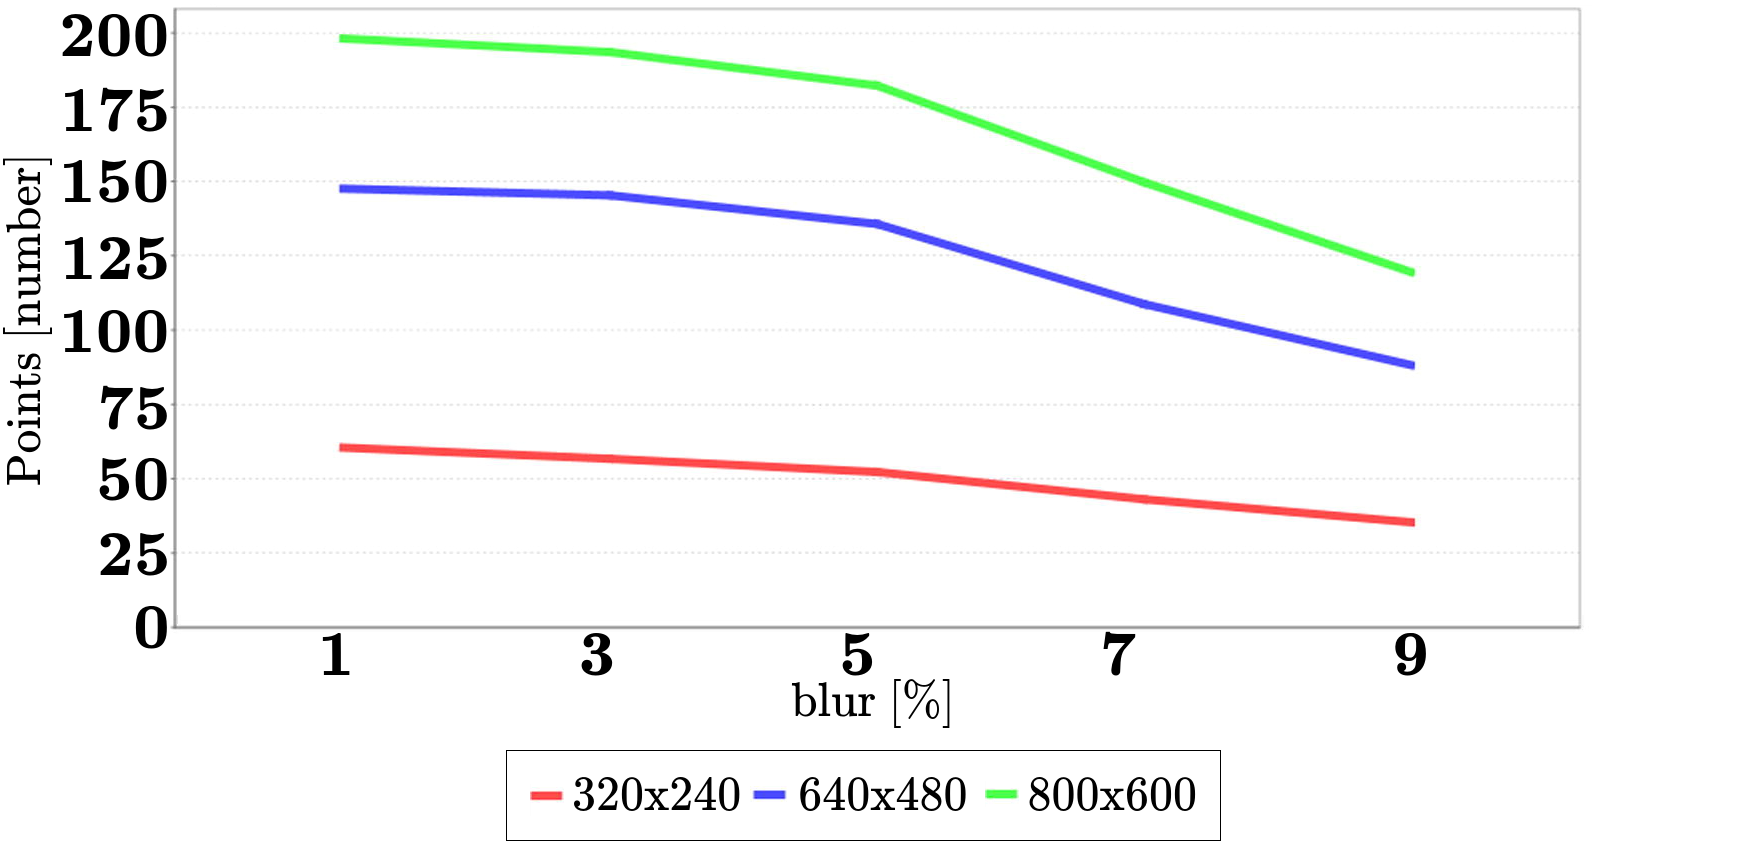
\includegraphics[width=\textwidth]{blurVsMatches}
	  \caption{Blur \emph{vs} matched points}\label{fig:cp01_blur_vs_matched}
        \end{subfigure}%    
        ~
        \begin{subfigure}[b]{0.45\textwidth}
	    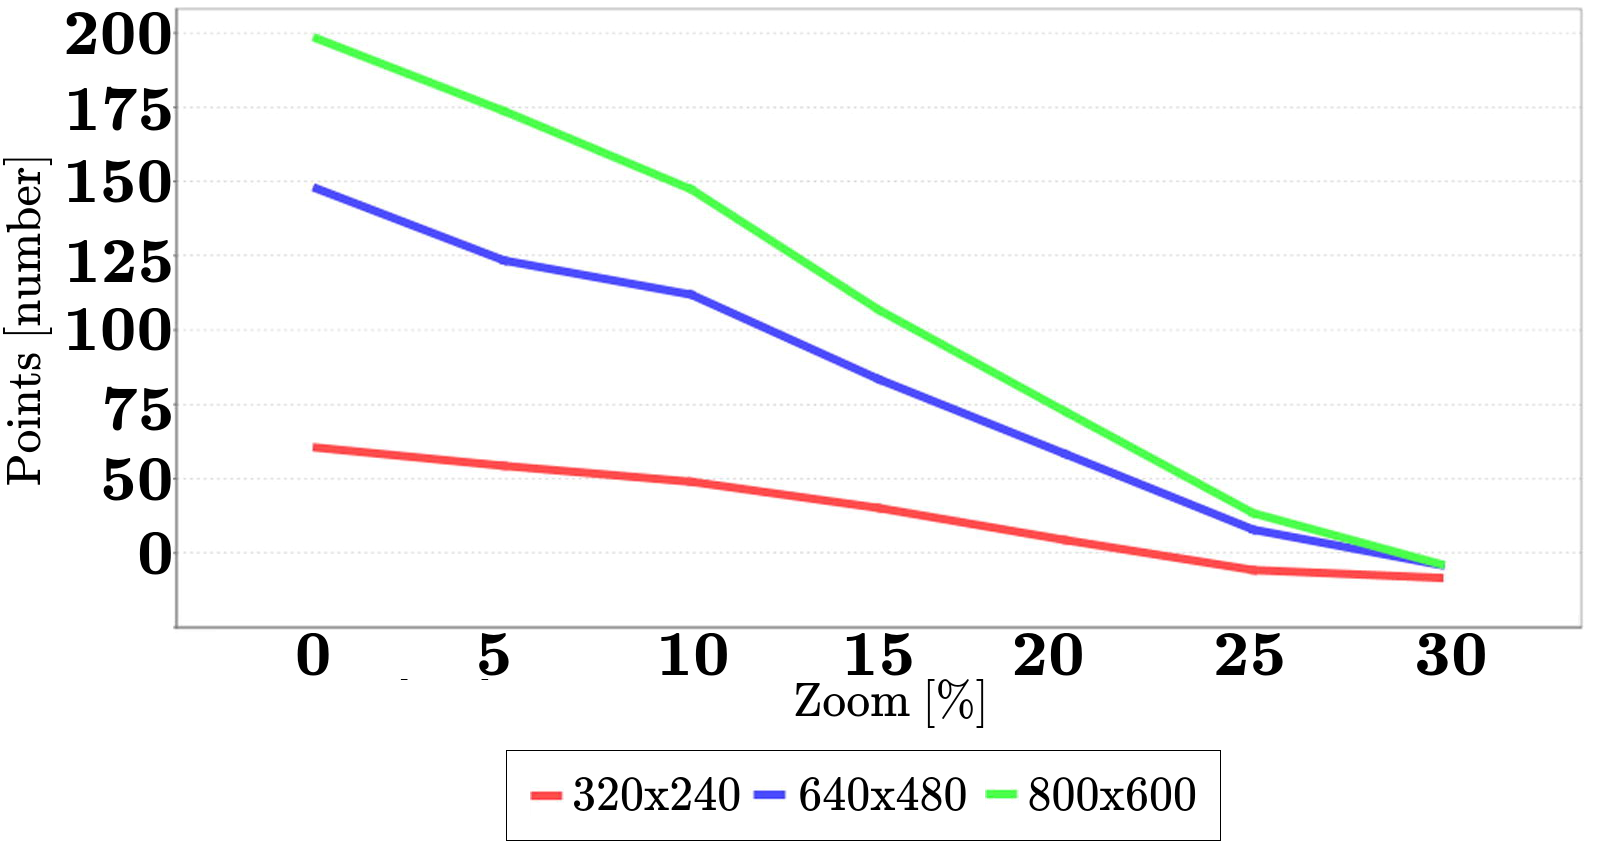
\includegraphics[width=\textwidth]{zoomVsMatches}
	  \caption{Zoom \emph{vs} matched points}\label{fig:cp01_zoom_vs_matched}
        \end{subfigure}%    
        \caption{Comparison of the number of matched points with several factors.}\label{fig:cp01_matching_results}
\end{figure*}

In this figure, four charts describing the difference of points matched attending on different variables are shown. Results obtained for the images at $320 \times 240$, $640 \times 480$ and $800 \times 600$ are represented by the red, blue and green lines, respectively. In those charts, we can see that the algorithm works properly when the euclidean distance between images is below 1\,m, and the angle difference is under 5-10\textdegree. Over this limit, the algorithm still works, but results are not so good. So we must be sure that our database is big enough to avoid going beyond these values. Anyway, the width of the road where the prototype will work is of about 3\,m and the driving direction usually does not change too much, so it is difficult to find a pair of images with such a big angular or euclidean difference.

Also different sized windows of Gaussian blurring have been passed over the images to test the robustness of the algorithm, as can be observed in the figure \ref{fig:cp01_blur_vs_matched}, where we notice that the algorithm is not too sensitive to the blurring. Similar results were obtained after applying different zoom percentages to the images used in tests (figure \ref{fig:cp01_zoom_vs_matched}).

As said before, to ensure that the method gives good results, the selection of the images is an important step in the whole process. A parameter that affects to several parts of the algorithm is the brightness difference. If this change is very big, the point matching stage could fail, and therefore the rest of the method. Also fake obstacles could appear. To minimize this effect, just images with a brightness difference falling under a certain threshold are retrieved from the database (see section \ref{ch:chapter01_01_01}). These brightness changes are strictly related to the hour in which they were obtained, but also there are a lot of factors that can affect, just like the weather, different shadows, etc. In the figure \ref{fig:cp01_brightness_vs_matches}, a chart shows how the number of points paired decreases as the brightness difference gets bigger.

\begin{figure}[t]
\centering
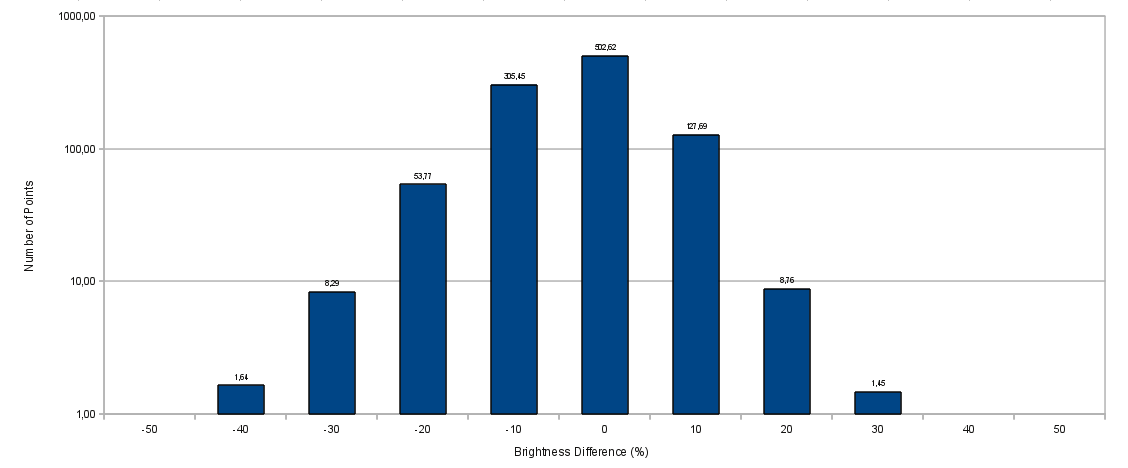
\includegraphics[width=\textwidth]{brightness_vs_matches}
\caption{Matches obtained related to the brightness difference of the input images.}\label{fig:cp01_brightness_vs_matches}
\end{figure}

In this chart, it is possible to appreciate that when the database image becomes darker, less point pairs are found. Virtually no control points are found over a difference of 50\% for darker images, and 40\% for brighter images.

From this test, we know that images 30\% darker or 20\% brighter than the current frame are not suitable for the method. Images in which the number of detected pairs is over 30 are adequate for this algorithm. Being conservative, a threshold of an absolute difference of 20\% is being used (parameter $\tau_{\mu}$ of equation \ref{eq:cp01_eligible_images_by_brightness}).

Medium and maximal covered areas of the images have been studied, too. Apart from having a lot of features matched, these features should be distributed in such a way that an area of the image as big as possible is covered. A comparison of the size of the areas covered at different image distances or angles is represented at figure \ref{fig:cp01_area_covered}. As can be seen, results are better for the nearest images, covering areas up to 90\% of the image.

\begin{figure*}[t]
\centering
  \begin{subfigure}[b]{0.45\textwidth}
  \centering
    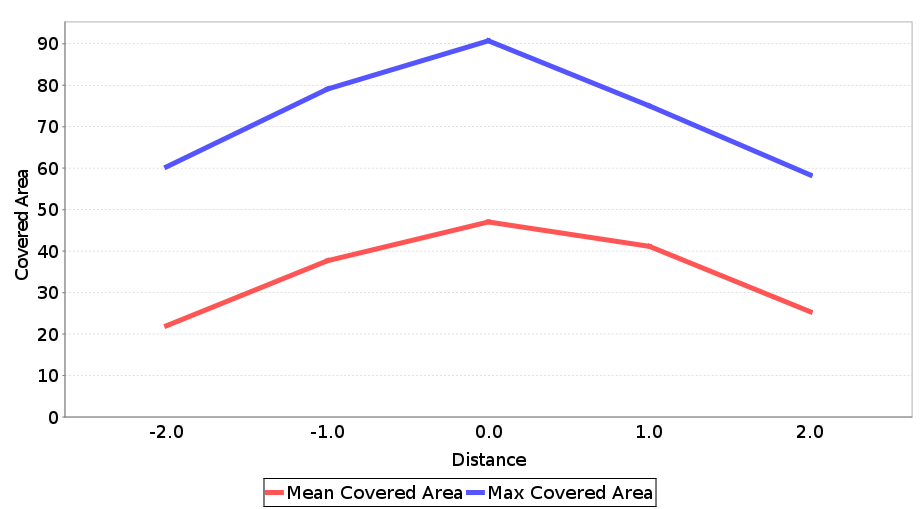
\includegraphics[width=\textwidth]{distance_vs_area}\label{fig:cp01_distance_vs_area}
  \end{subfigure}%
  ~
  \begin{subfigure}[b]{0.45\textwidth}
    \centering
    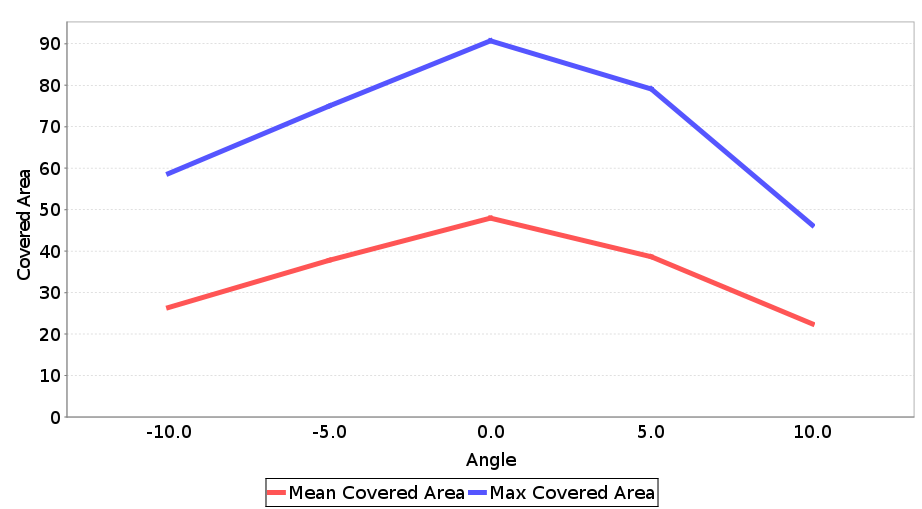
\includegraphics[width=\textwidth]{angle_vs_area}\label{fig:cp01_angle_vs_area}
  \end{subfigure}%
  \caption{Size of the covered area of the image related to the euclidean distance (upper image) and angle difference (lower image) between $I_{RT}$ and $I_{DB}$.}\label{fig:cp01_area_covered}
\end{figure*}

In the other hand, to test the goodness of the adjustment made by the algorithm, images with no obstacles were used. If the algorithm works well, a low number of pixels marked as change should be obtained. For the images tested, the number of points detected as changes were under 5\% (there are always differences due to noise or bad adjustments, but in many cases they are usually dispersed around the image, without making clusters).

\subsection{Obstacle detection}\label{ch:chapter01_02_02}

The final objective of the method is the detection of the obstacles in the environment of the vehicle. In order to evaluate this part of the algorithm, we have generated by hand the ground truth for a sequence recorded in the testing area. By comparing this ground truth with the obstacles found by the algorithm, we obtained the results in table \ref{table:cp01_fp_and_fp}.

\begin{table}[h]
\begin{center}
\begin{tabular}{|c|c|c|c|}
 \hline
 Distance (m) & Angle (\textdegree) & False positives (\%)  & False negatives (\%) \\
 \hline
 −1 & 0 & 9.76 & 16.67 \\
−1 & 5 & 12.50 & 8.33 \\
−1 & 10 & 15.00 & 16.67 \\
0 & −10 & 0 & 22.22 \\
0 & −5 & 13.95 & 8.33 \\
0 & 0 & 4.88 & 2.78 \\
0 & 5 & 8.33 & 13.89 \\
0 & 10 & 11.54 & 38.89 \\
1 & −10 & 28.57 & 19.44 \\
1 & −5 & 14.29 & 8.33 \\
1 & 0 & 12.20 & 11.11 \\
 \hline
\end{tabular}
\end{center}
\caption{False positive and false negative results related to the distance and the angle between the compared images.}\label{table:cp01_fp_and_fp}
\end{table}

As seen, the rate of false positives is quite good inside the expected limits, obtaining the best results when the angle difference is low. The response obtained for images with an angle difference over 10\textdegree is not as good. This reflects the importance of a well populated database: if the number of images increases, the probability of having images with a big angle difference decreases. However, as the road where the prototype will travel is not too wide, the probability of a higher difference is small. Best results are obtained in the case where the distance and angle to the sensed image is 0, as it would be expected.

\subsection{Timing results}\label{ch:chapter01_02_03}

One of the most critical parameters taken into account for the development of the method is the computational time that the algorithm needs for its execution. In figure \ref{fig:cp01_times}, a chart shows the times obtained when executing the method for some image pairs, ordered by the total time required.

\begin{figure}[t]
\centering
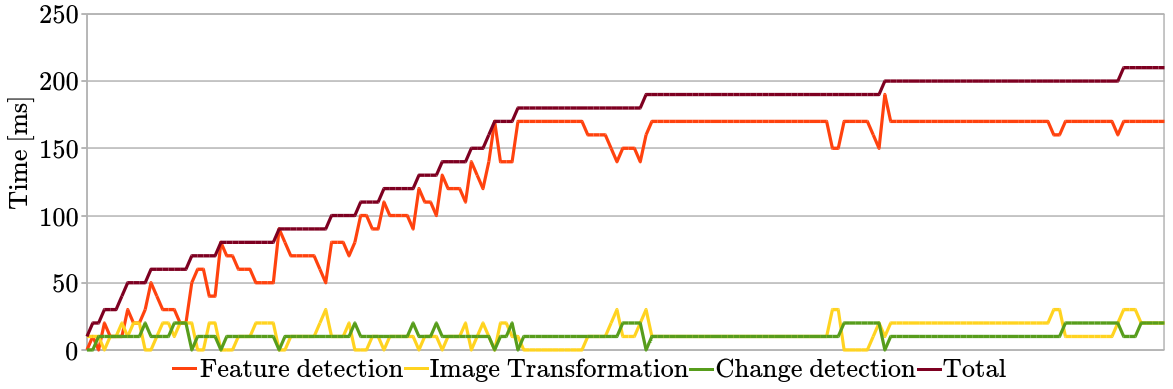
\includegraphics[width=\textwidth]{times}
\caption{Times obtained after the execution of a big sequence of images, ordered by the total time measured.}\label{fig:cp01_times}
\end{figure}

As shown there, almost all the times are below 200\,ms, enough time to allow the algorithm to avoid loosing data reported by the \ac{GPS}, except from a small percentage of image pairs, with a maximal execution time of 210\,ms. However, the number of images over the threshold of 200\,ms is very small and these times are not extremely big. It is easy to notice that the part of the algorithm which consumes more time is that for the feature extraction and optical flow steps. The more features that are selected, the more time needed. To prevent the method from expending too much time in this stage, the number of features that can be selected is limited. In the other hand, image transformation and change detection methods have constant times, with a maximal computational time of 30\,ms and 20\,ms, respectively.

\subsection{Qualitative results}\label{ch:chapter01_02_04}

In this section, we will observe some examples of the detections performed by the method. In figure \ref{fig:cp01_pipeline_example}, we can observe some of the intermediate steps in the pipeline of the method. The first two columns represent the images $I_{DB}$ and $I_{RT}$, respectively. There, the features found and matched in both images are represented with a color code, assigning the same random color for a point in the first image and its associated point in the second. In the third column, the output obtained after applying the \ac{PCA} to the aligned images is shown, and in the last column, the detected objects are represented. As we can see, there are many obstacles detected in the bushes next to the road and due to some occlusions. Anyway, as we are using the road mask (represented in gray), we can discard them and limit the detection to the objects lying in the ground, so this effect (occlusions or small changes in the static objects) is negligible.

\begin{figure*}[t]
        \centering
        \begin{subfigure}[b]{0.24\columnwidth}
	    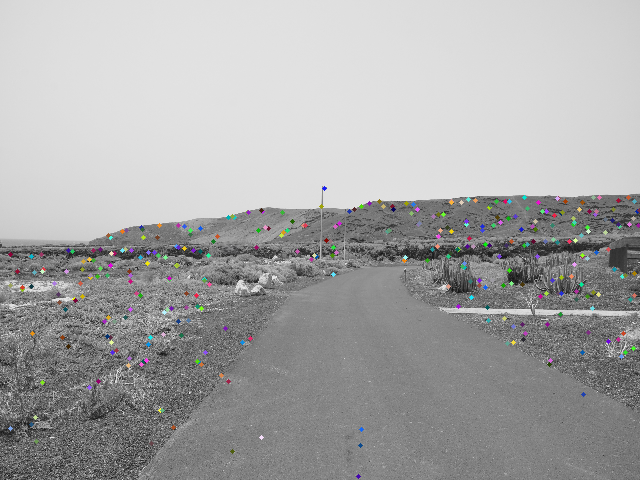
\includegraphics[width=\textwidth]{pipeline/fig5}\label{fig:pipelineA_1}
        \end{subfigure}% 
        ~
        \begin{subfigure}[b]{0.24\columnwidth}
	    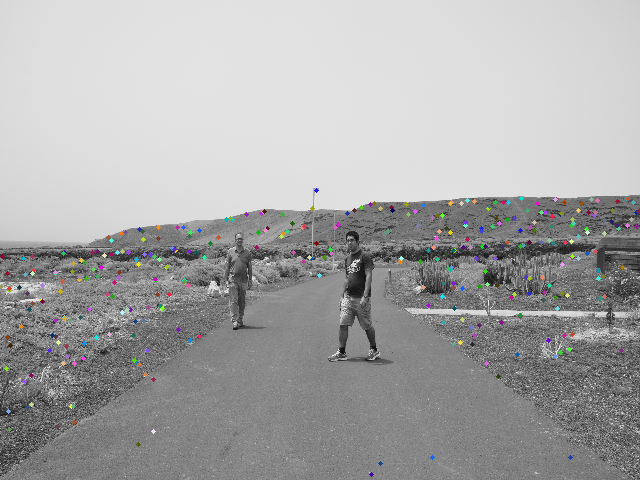
\includegraphics[width=\textwidth]{pipeline/fig4}\label{fig:pipelineA_2}
        \end{subfigure}%       
        ~
        \begin{subfigure}[b]{0.24\columnwidth}
	    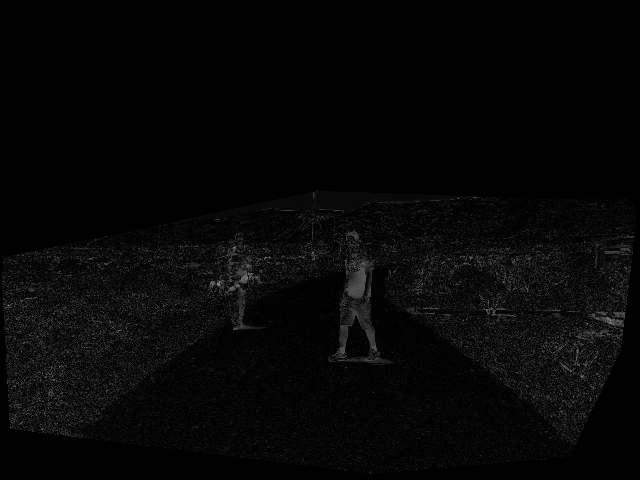
\includegraphics[width=\textwidth]{pipeline/fig2}\label{fig:pipelineA_3}
        \end{subfigure}%    
        ~
        \begin{subfigure}[b]{0.24\columnwidth}
	    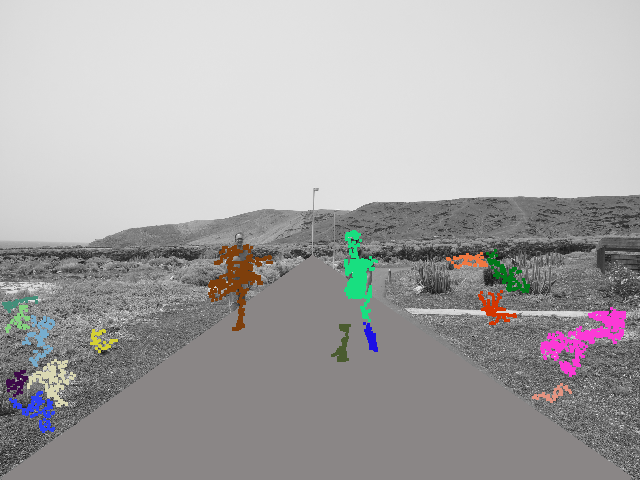
\includegraphics[width=\textwidth]{pipeline/fig3}\label{fig:pipelineA_4}
        \end{subfigure}%
        \\
        \begin{subfigure}[b]{0.24\columnwidth}
	    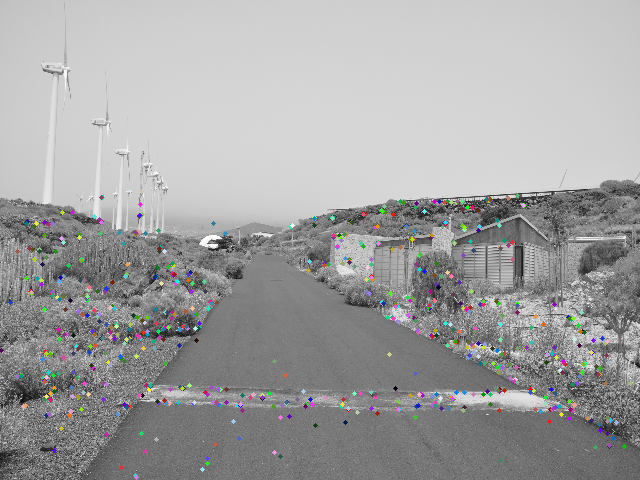
\includegraphics[width=\textwidth]{pipeline2/fig2}\label{fig:pipelineB_1}
        \end{subfigure}% 
        ~
        \begin{subfigure}[b]{0.24\columnwidth}
	    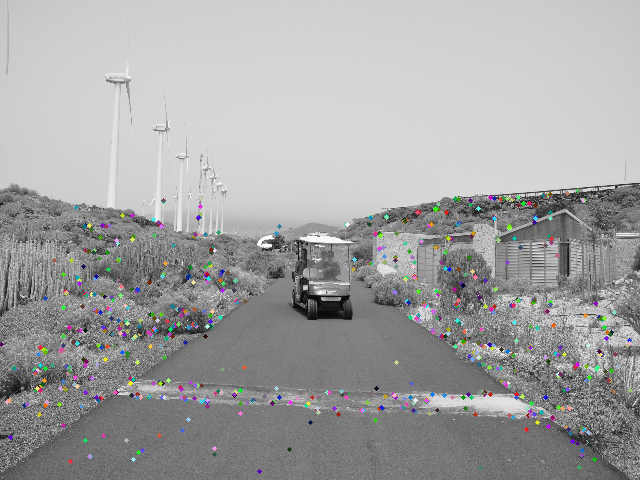
\includegraphics[width=\textwidth]{pipeline2/fig1}\label{fig:pipelineB_2}
        \end{subfigure}%       
        ~
        \begin{subfigure}[b]{0.24\columnwidth}
	    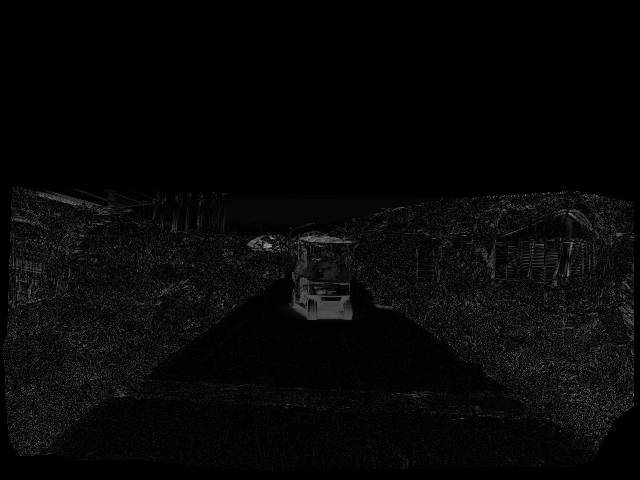
\includegraphics[width=\textwidth]{pipeline2/fig4}\label{fig:pipelineB_3}
        \end{subfigure}%    
        ~
        \begin{subfigure}[b]{0.24\columnwidth}
	    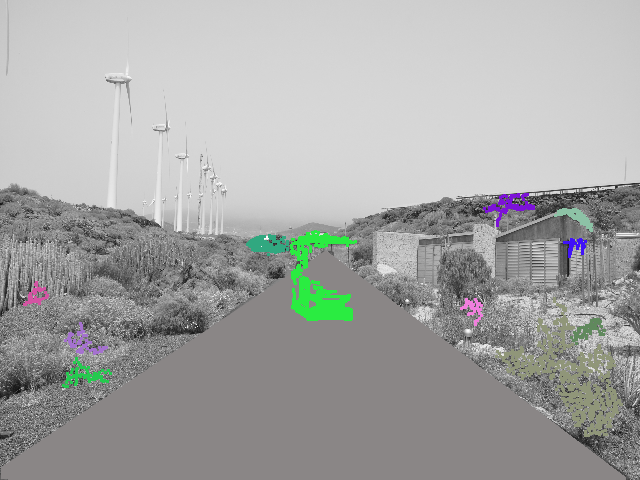
\includegraphics[width=\textwidth]{pipeline2/fig5}\label{fig:pipelineB_4}
        \end{subfigure}%
        \caption{Two examples of the pipeline followed by the method.}\label{fig:cp01_pipeline_example}
\end{figure*}

Also, in figure \ref{fig:cp01_sequence_example}, we can see some frames of a sequence in which a vehicle is being detected using this method. As seen, the method is able to detect the obstacle even when it is far away. We just detect the bottom of the vehicle because the roof of the car is out of the road mask. This sequence was recorded inside the area in which the vehicle will be driving, at ITER's facilities.

\begin{figure*}[h!]
        \centering
        \begin{subfigure}[b]{0.24\columnwidth}
	    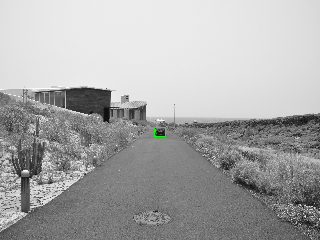
\includegraphics[width=\textwidth]{sequence/seq1}\label{fig:seq1}
        \end{subfigure}% 
        ~
        \begin{subfigure}[b]{0.24\columnwidth}
	    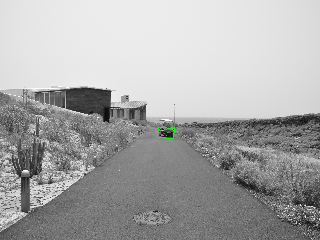
\includegraphics[width=\textwidth]{sequence/seq2}\label{fig:seq2}
        \end{subfigure}%       
        ~
        \begin{subfigure}[b]{0.24\columnwidth}
	    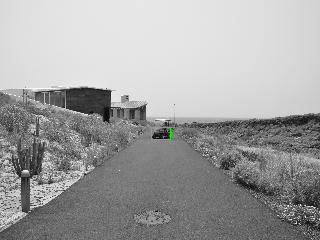
\includegraphics[width=\textwidth]{sequence/seq3}\label{fig:seq3}
        \end{subfigure}%    
        ~
        \begin{subfigure}[b]{0.24\columnwidth}
	    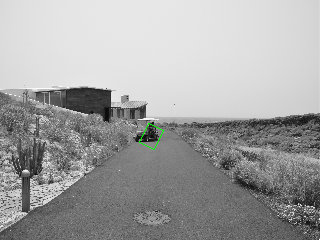
\includegraphics[width=\textwidth]{sequence/seq4}\label{fig:seq4}
        \end{subfigure}%
        \\
        \begin{subfigure}[b]{0.24\columnwidth}
	    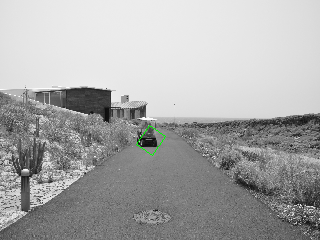
\includegraphics[width=\textwidth]{sequence/seq5}\label{fig:seq5}
        \end{subfigure}% 
        ~
        \begin{subfigure}[b]{0.24\columnwidth}
	    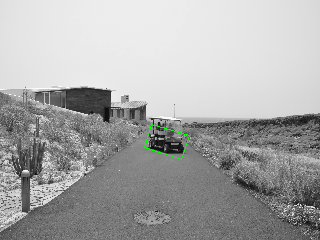
\includegraphics[width=\textwidth]{sequence/seq6}\label{fig:seq6}
        \end{subfigure}%       
        ~
        \begin{subfigure}[b]{0.24\columnwidth}
	    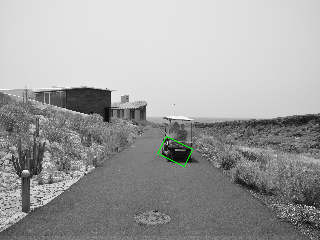
\includegraphics[width=\textwidth]{sequence/seq7}\label{fig:seq7}
        \end{subfigure}%    
        ~
        \begin{subfigure}[b]{0.24\columnwidth}
	    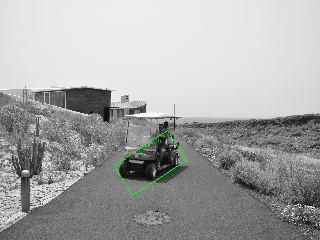
\includegraphics[width=\textwidth]{sequence/seq8}\label{fig:seq8}
        \end{subfigure}%
        \caption{A sequence in which a vehicle is detected.}\label{fig:cp01_sequence_example}
\end{figure*}

\FloatBarrier
 
\graphicspath{{./images/chapter02/bmps/}{./images/chapter02/vects/}{./images/chapter02/}}
\section{Non-rigid contour tracking}\label{ch:chapter02_02}

In this section, related to the methods described in chapter \ref{ch:chapter02}, four different groups of experiments have been performed. Two of them aiming at choosing the best algorithm combination to be used in the stages of foreground segmentation and contour flow selection. Then, we fine tune those algorithms, in terms of the parameter values that will be used. In the last group of experiments, we compare the output of our method with the output obtained by both a Microsoft Kinect\textregistered and by a Computer Vision based method.

\subsection{Foreground segmentation}\label{ch:chapter02_02_01}

For the evaluation of the methods taken into account for the foreground segmentation stage, the accuracy metrics considered were the \textit{Recall}, \textit{Precision}, \textit{$F_1$} and \textit{Similarity} \citep{maddalena2008self}, which are used as follows:

\begin{equation}\label{eq_Recall}
Recall = { tp \over { tp + fn } }
\end{equation}
\begin{equation}\label{eq_Precision}
Precision = { tp \over { tp + fp } }
\end{equation}
\begin{equation}\label{eq_F1}
F_1 = { {2 * Recall * Precision} \over {Recall + Precision} }
\end{equation}
\begin{equation}\label{eq_Similarity}
Similarity = { tp \over { tp + fn + fp } },
\end{equation}

where $tp$, $tn$, $fp$ and $fn$ denote the number of true positives, true negatives, false positives and false negatives, respectively. $(fp + tn)$ indicates the total number of pixels representing the background in an image, while $(tp + fn)$ is the total number of pixels representing the foreground.
These measures where tested using the sequences of SZTAKI Surveillance Benchmark Set \citep{benedek2008bayesian}, obtaining the results shown at figure \ref{fig:cp02_chartsFG}.

\begin{figure*}[t]
        \centering
        \begin{subfigure}[b]{0.5\textwidth}
                \centering
                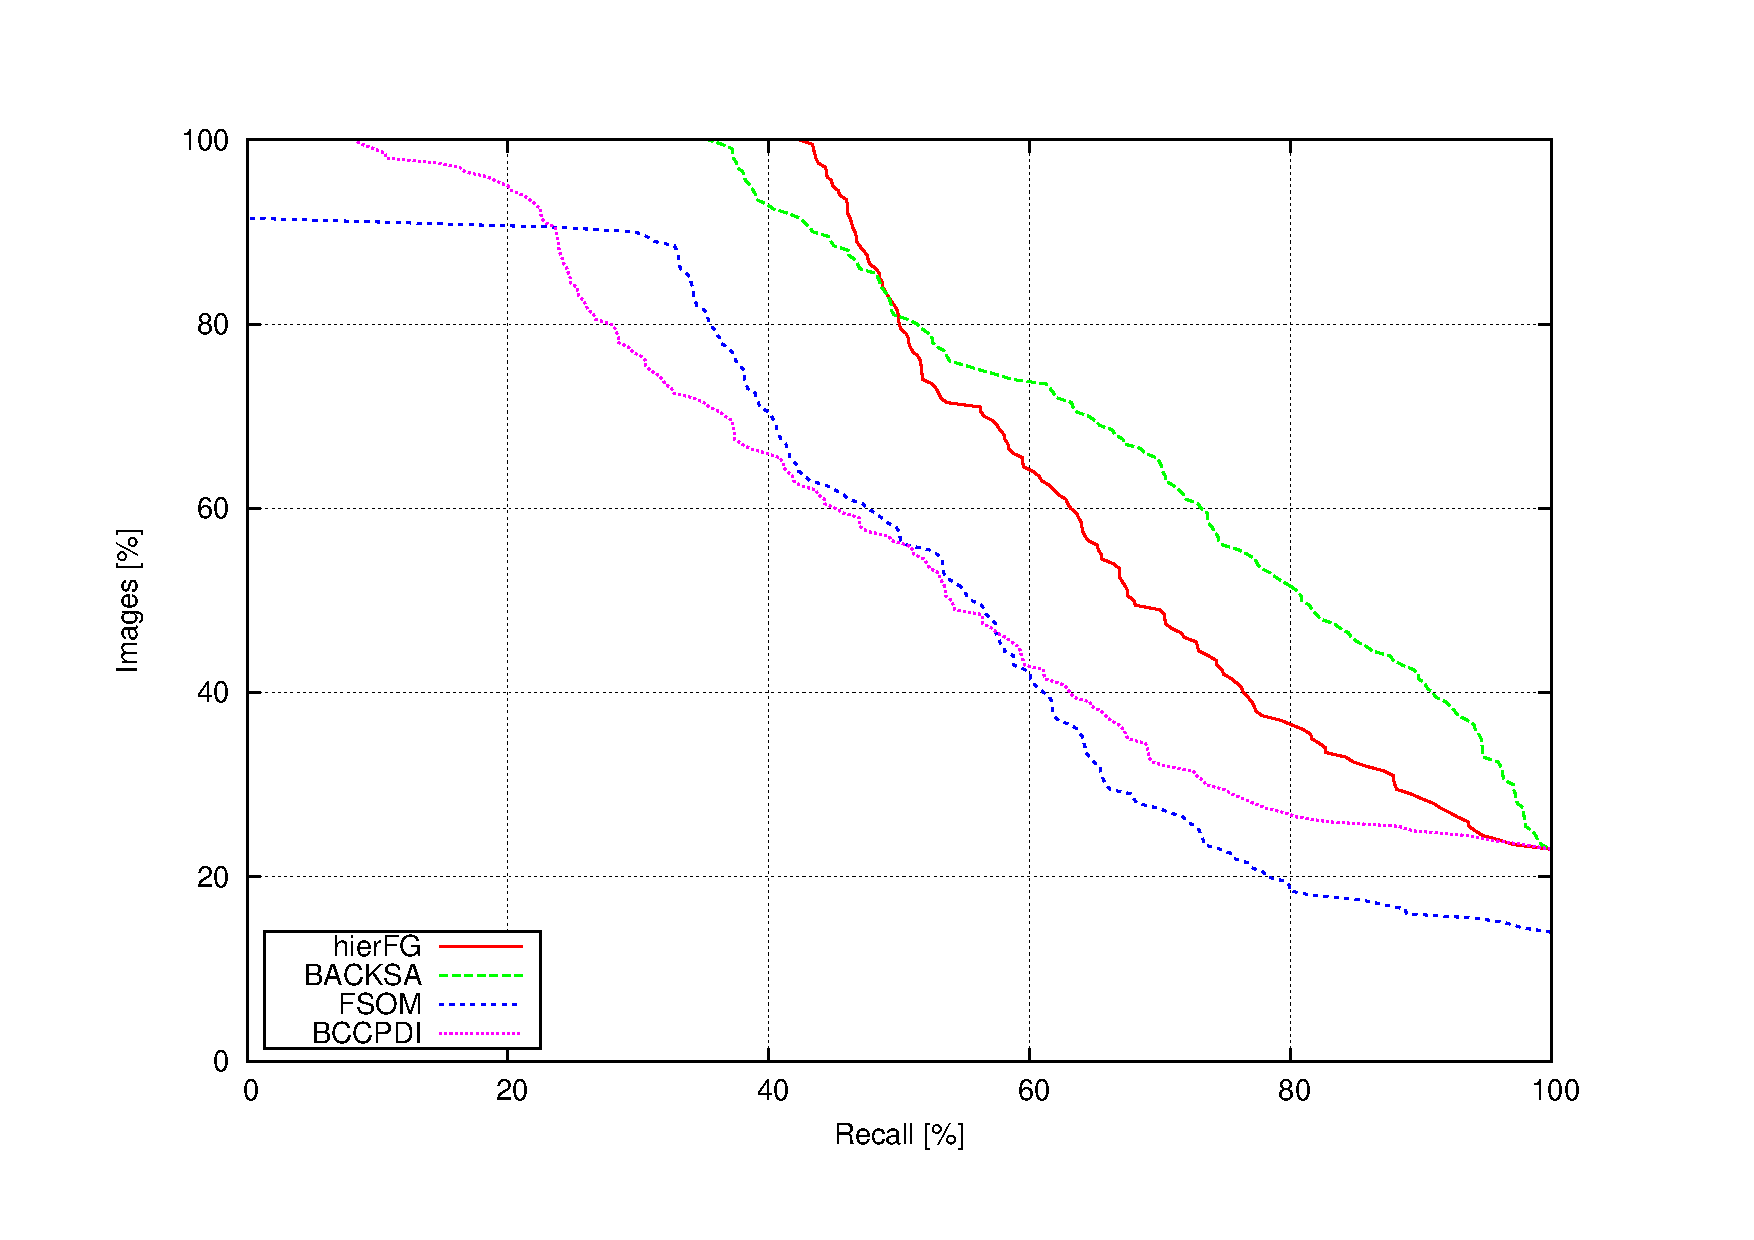
\includegraphics[width=\textwidth, trim=50 40 80 50,clip]{fig9.pdf}
                \caption{Recall}
                \label{fig:cp02_recallChart}
        \end{subfigure}%        
        ~ %add desired spacing between images, e. g. ~, \quad, \qquad etc.
          %(or a blank line to force the subfigure onto a new line)
        \begin{subfigure}[b]{0.5\textwidth}
                \centering
                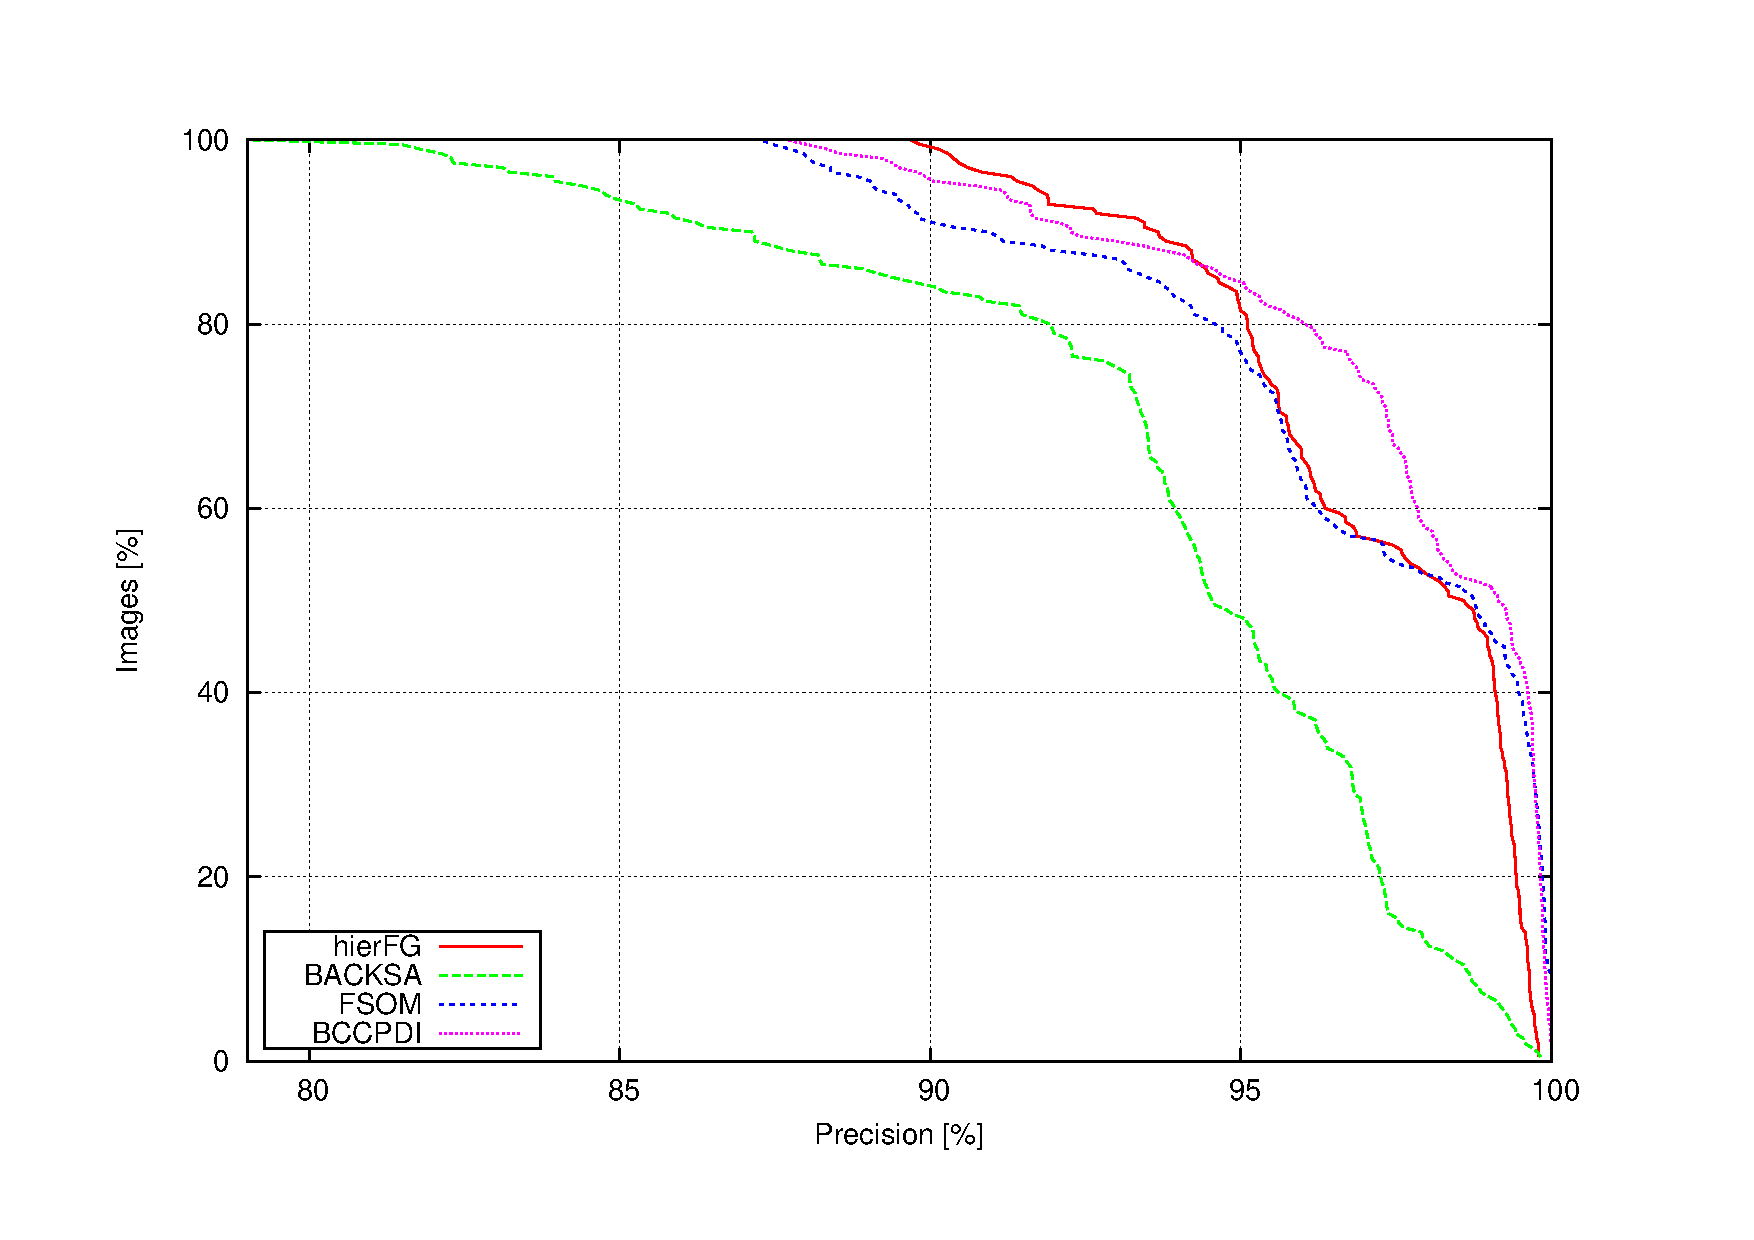
\includegraphics[width=\textwidth, trim=50 40 80 50,clip]{fig10.pdf}
                \caption{Precision}
                \label{fig:cp02_precisionChart}
        \end{subfigure}%
        
%         ~ %add desired spacing between images, e. g. ~, \quad, \qquad etc.
          %(or a blank line to force the subfigure onto a new line)
        \begin{subfigure}[b]{0.5\textwidth}
                \centering
                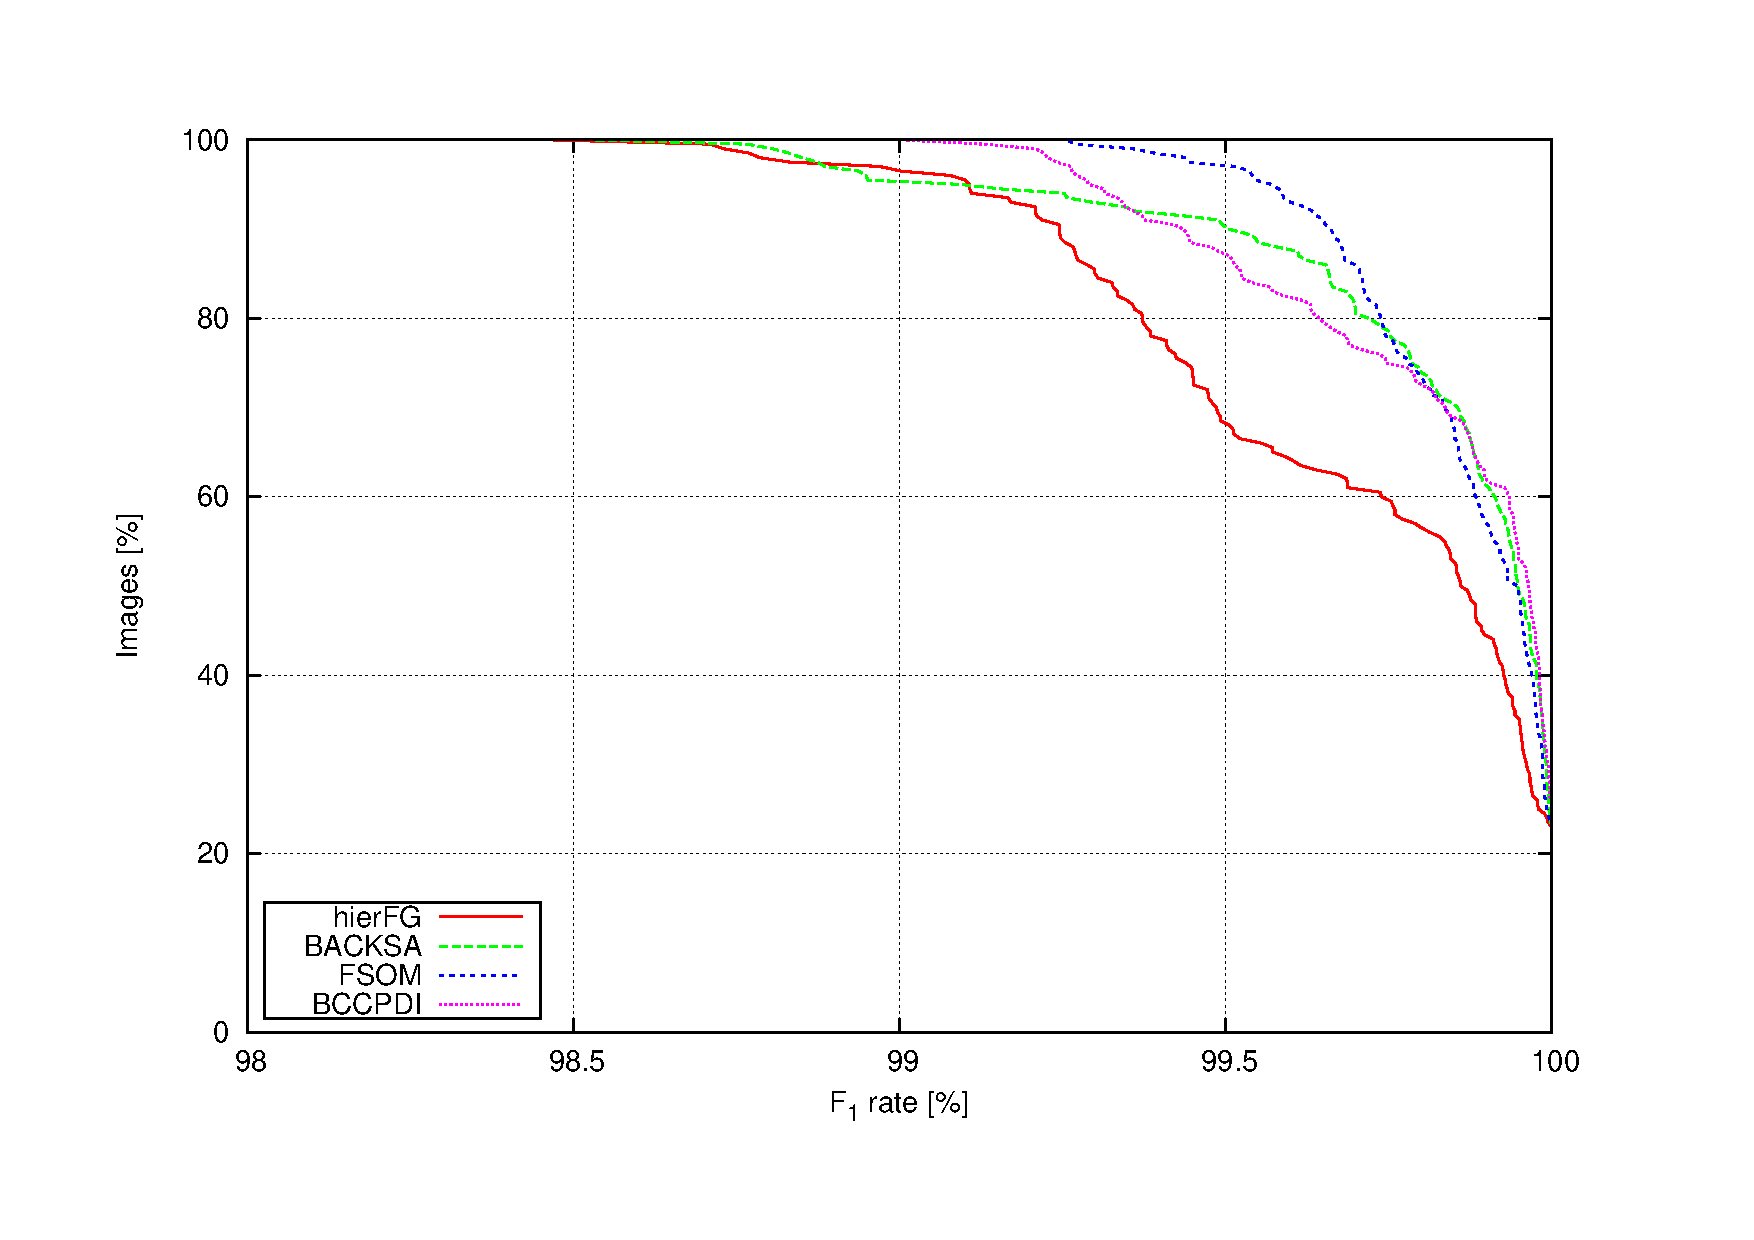
\includegraphics[width=\textwidth, trim=50 40 80 50,clip]{fig11.pdf}
                \caption{$F_1$}
                \label{fig:cp02_f1Chart}
        \end{subfigure}%
        ~ %add desired spacing between images, e. g. ~, \quad, \qquad etc.
          %(or a blank line to force the subfigure onto a new line)
        \begin{subfigure}[b]{0.5\textwidth}
                \centering
                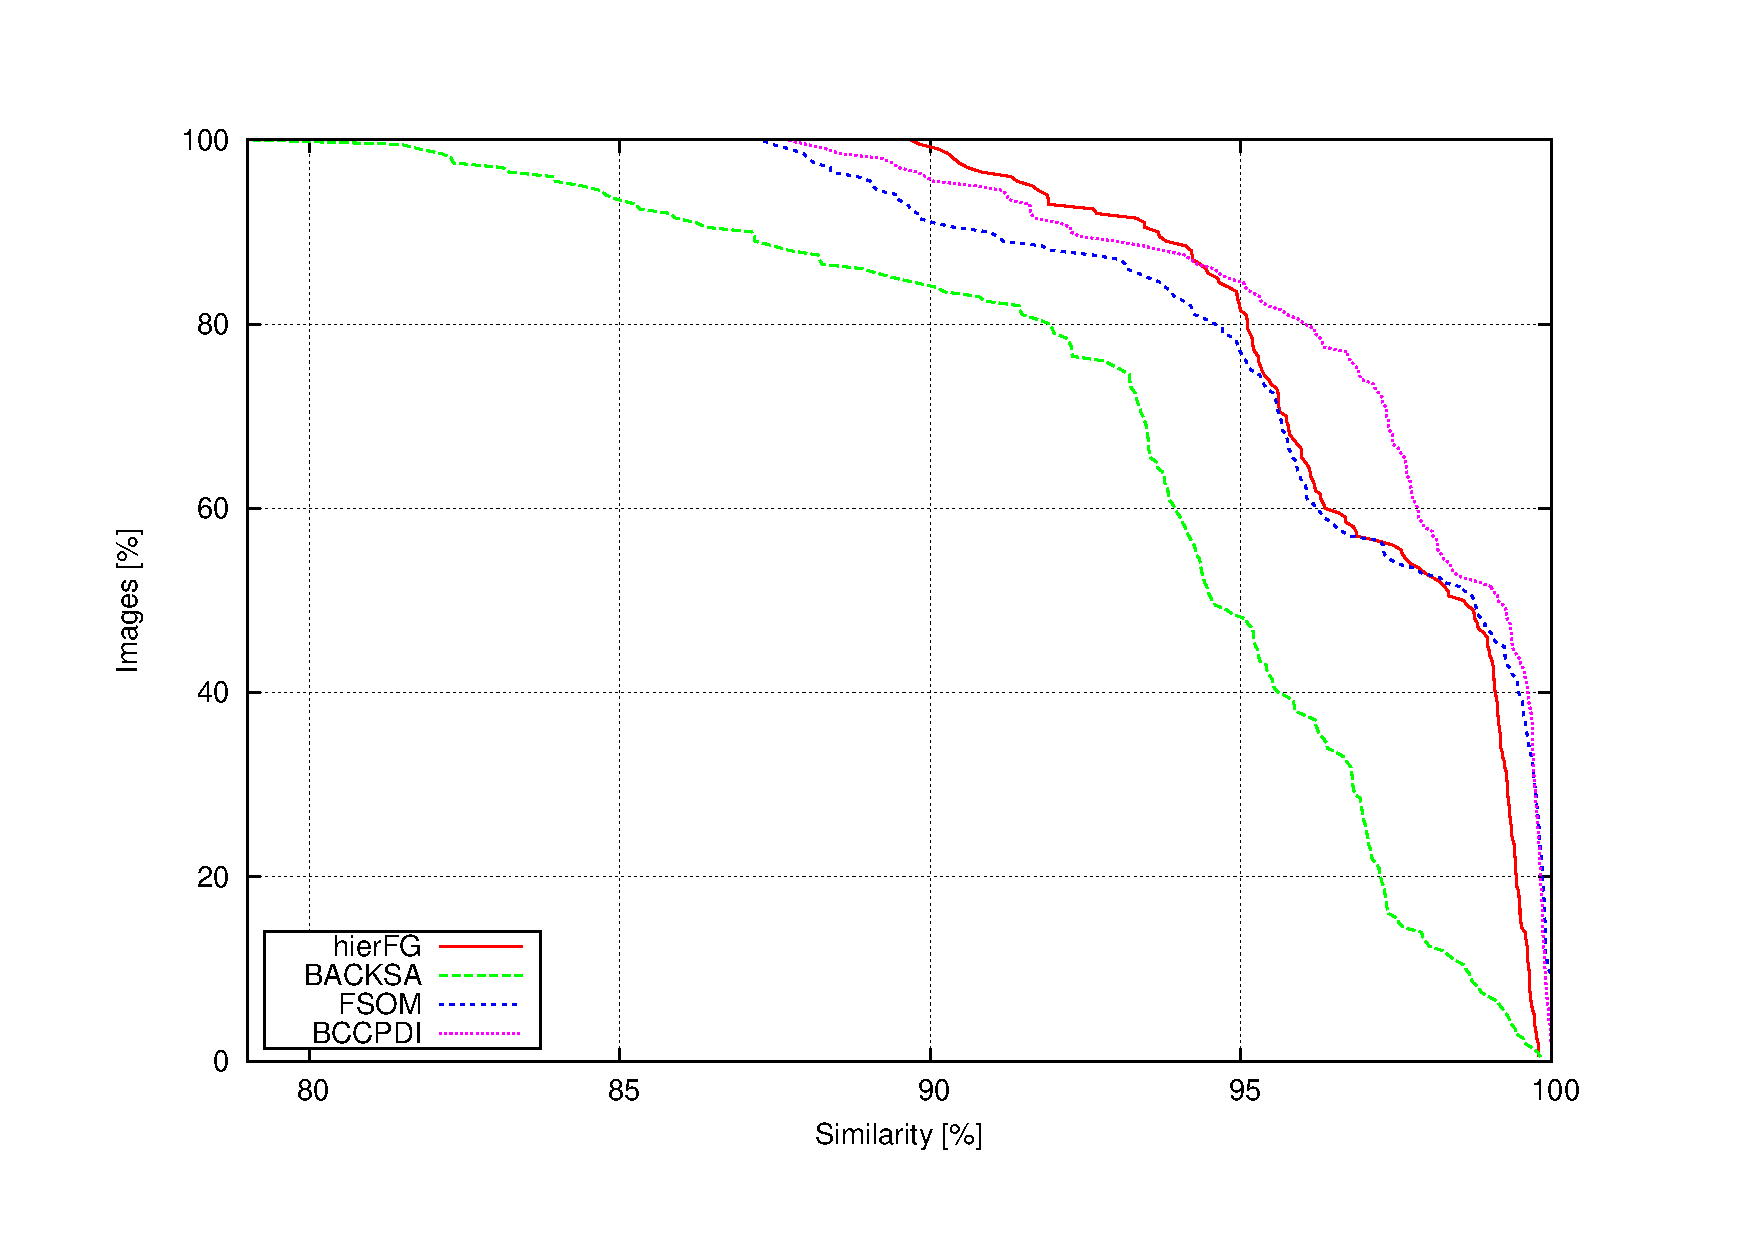
\includegraphics[width=\textwidth, trim=50 40 80 50,clip]{fig12.pdf}
                \caption{Similarity}
                \label{fig:cp02_similarityChart}
        \end{subfigure}
        \caption{Values obtained for the foreground detection tested algorithms.}\label{fig:cp02_chartsFG}
\end{figure*}

\begin{table}[t]
\begin{center}
\resizebox{0.5\columnwidth}{!} {
\begin{tabular}{|l|c|c|c|c|}
\hline
Method & Recall & Precision & $F_1$ & Similarity \\
\hline
BACKSA & \textbf{76.72} \% & 93.92 \% & 99.82 \% & 93.77 \% \\
FSOM & 55.29 \% & 96.88 \% & \textbf{99.87} \% & 96.76 \% \\
hierFG & 71.89 \% & 97.15 \% & 99.69 \% & 96.87 \% \\
BCCPDI & 57.87 \% & \textbf{97.61} \% & 99.83 \% & \textbf{97.46} \% \\
\hline
\end{tabular}
}
\caption{Foreground detection methods. Average results.}\label{table:fgAverage}
\end{center}
\end{table}

Figure \ref{fig:cp02_recallChart} shows the percentage of images (Y-axis) that are under a certain value of recall (X-axis) 
for each algorithm. As seen, best results are obtained for the BACKSA method, followed by the hierFG algorithm.  FSOM 
and BCCPDI methods have not so good results. Having a look to the table \ref{table:fgAverage}, this behavior is also 
reflected in the average of the measures of all the images.

In figure \ref{fig:cp02_precisionChart} it is observable that the best precision is shown for the BCCPDI, which does not 
differ too much from the results obtained for the hierFG and FSOM algorithms. It is noticeable also that, for these 
three algorithms, the lowest value is above an 87\% of precision. Also, if having a look at table \ref{table:fgAverage}, 
the average precision values for hierFG and BCCPDI are above a 97\%.

In the chart shown at figure \ref{fig:cp02_f1Chart}, results are also quite good, being the minimum value for all the 
algorithms above an 98\%, and where the best values are obtained for FSOM, not too far from the values of the BACKSA and 
BCCPDI algorithms. Despite hierFG falls a little faster than the other three algorithms, results are also good for this 
algorithm. This behavior is reflected by the values represented in table \ref{table:fgAverage}, where all the averages 
for this measure are above a 99\%.

Finally, in the chart depicted in figure \ref{fig:cp02_similarityChart}, hierFG, FSOM and BCCPDI show a similar behavior, 
although the response of BCCPDI is slightly better. Measures for BACKSA are not so good, being almost a 60\% of the 
tested images below a 95\% of similarity. Again, table \ref{table:fgAverage} confirm these data, showing that best 
results are obtained for BCCPDI.

As seen, results are quite similar. In table \ref{table:fgAverage}, it is possible to see that hierFG is the most 
constant, with high values for all the measures. However, BCCPDI is a good candidate also, despite of the not so good 
recall. There is not a clear candidate, so final decision must be performed based on the aspect of the retrieved masks. 
In figure \ref{fig:cp02_fgMasks} it is possible to see several examples of the obtained images.

\begin{figure*}[t]
        \centering
        \begin{subfigure}[b]{0.19\textwidth}
                \centering
                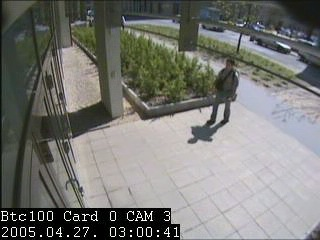
\includegraphics[width=\textwidth]{fig13.jpg}
                \caption{Original}
                \label{fig:cp02_originalMask}
        \end{subfigure}%        
        ~ %add desired spacing between images, e. g. ~, \quad, \qquad etc.
          %(or a blank line to force the subfigure onto a new line)
        \begin{subfigure}[b]{0.19\textwidth}
                \centering
                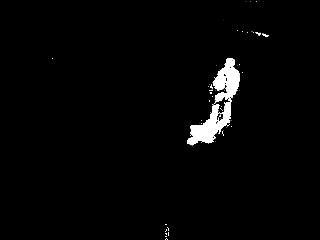
\includegraphics[width=\textwidth]{fig14.jpg}
                \caption{BACKSA}
                \label{fig:cp02_backsaMask}
        \end{subfigure}%
        ~ %add desired spacing between images, e. g. ~, \quad, \qquad etc.
          %(or a blank line to force the subfigure onto a new line)
        \begin{subfigure}[b]{0.19\textwidth}
                \centering
                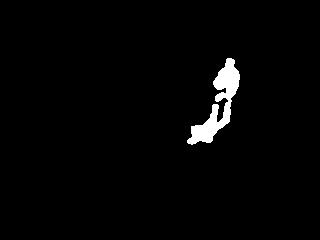
\includegraphics[width=\textwidth]{fig15.jpg}
                \caption{FSOM}
                \label{fig:cp02_fsomMask}
        \end{subfigure}%
        ~ %add desired spacing between images, e. g. ~, \quad, \qquad etc.
          %(or a blank line to force the subfigure onto a new line)
        \begin{subfigure}[b]{0.19\textwidth}
                \centering
                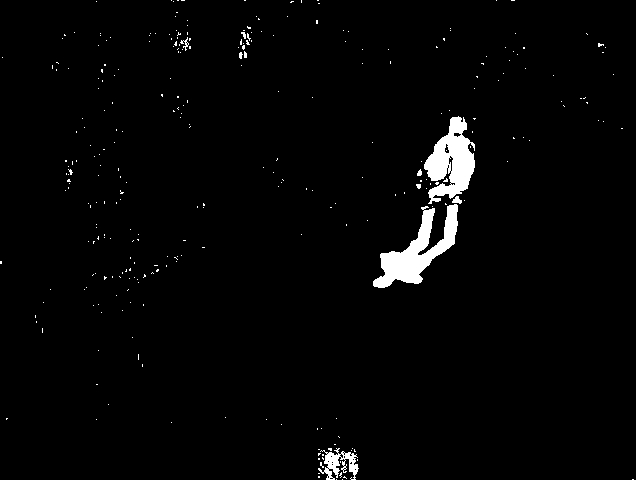
\includegraphics[width=\textwidth]{fig16.jpg}
                \caption{hierFG}
                \label{fig:cp02_hierFGmask}
        \end{subfigure}%
	~ %add desired spacing between images, e. g. ~, \quad, \qquad etc.
          %(or a blank line to force the subfigure onto a new line)
	\begin{subfigure}[b]{0.19\textwidth}
                \centering
                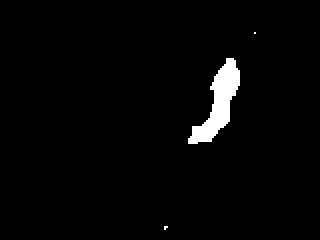
\includegraphics[width=\textwidth]{fig17.jpg}
                \caption{BCCPDI}
                \label{fig:cp02_bccpdiMask}
        \end{subfigure}%

        \caption{Masks obtained for the foreground extraction tested algorithms}\label{fig:cp02_fgMasks}
\end{figure*}

As can be seen, the cleanest images are obtained for the FSOM and BCCPDI algorithms. Also, borders of the silhouettes 
are softer, making them suitable for the proposed algorithm. However, FSOM seems to show holes in some of the frames. 
Surprisingly, the noisiest one is hierFG, which in contrast is the one that in table \ref{table:fgAverage} seemed to be 
the most stable. The image could be cleaned after post-processing it, but nevertheless, it still seems to be more 
sensitive to moving backgrounds.

Based on the results, the most promising algorithms are FSOM and BCCPDI. We finally decided to use BCCPDI for our method 
as FSOM produces holes in some frames, which is not appropriate behavior for the application.

\subsection{Nonrigid point set matching}\label{ch:chapter02_02_02}

In order to select the best of the tested algorithms, several tests were performed using the data provided by 
\cite{chui2000new}. Using this dataset, the error of the obtained registration and the number of mismatches obtained for 
each test was calculated. Also, as the bottleneck of this application is in the point set registration algorithms, we 
tested the relative computing time needed by each algorithm.

\begin{figure*}[t]
        \centering
        \begin{subfigure}[b]{0.45\columnwidth}
                \centering
                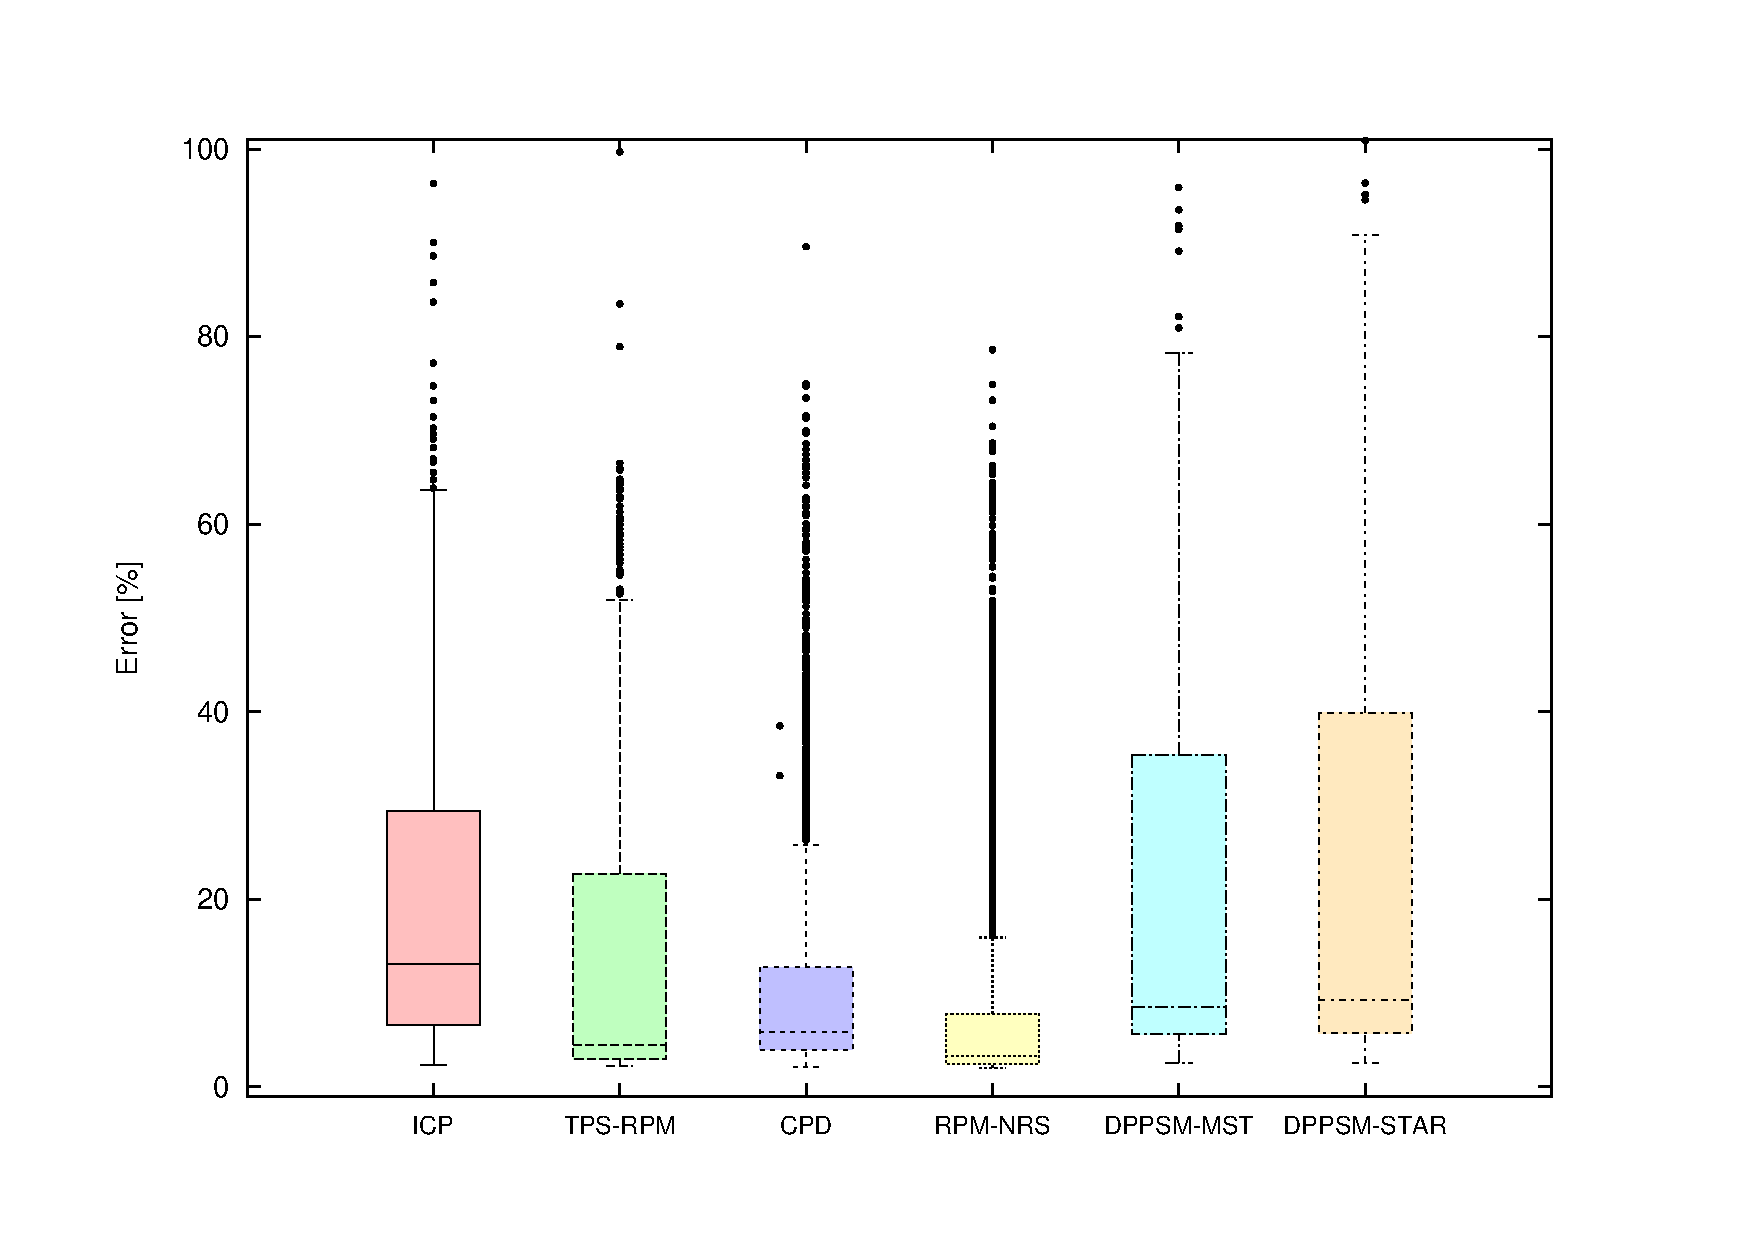
\includegraphics[width=\textwidth, trim=50 40 80 50,clip]{fig18.pdf}
                \caption{Error}
                \label{fig:cp02_errorChart}
        \end{subfigure}%     
%         ~ %add desired spacing between images, e. g. ~, \quad, \qquad etc.
          %(or a blank line to force the subfigure onto a new line)
        \begin{subfigure}[b]{0.45\columnwidth}
                \centering
                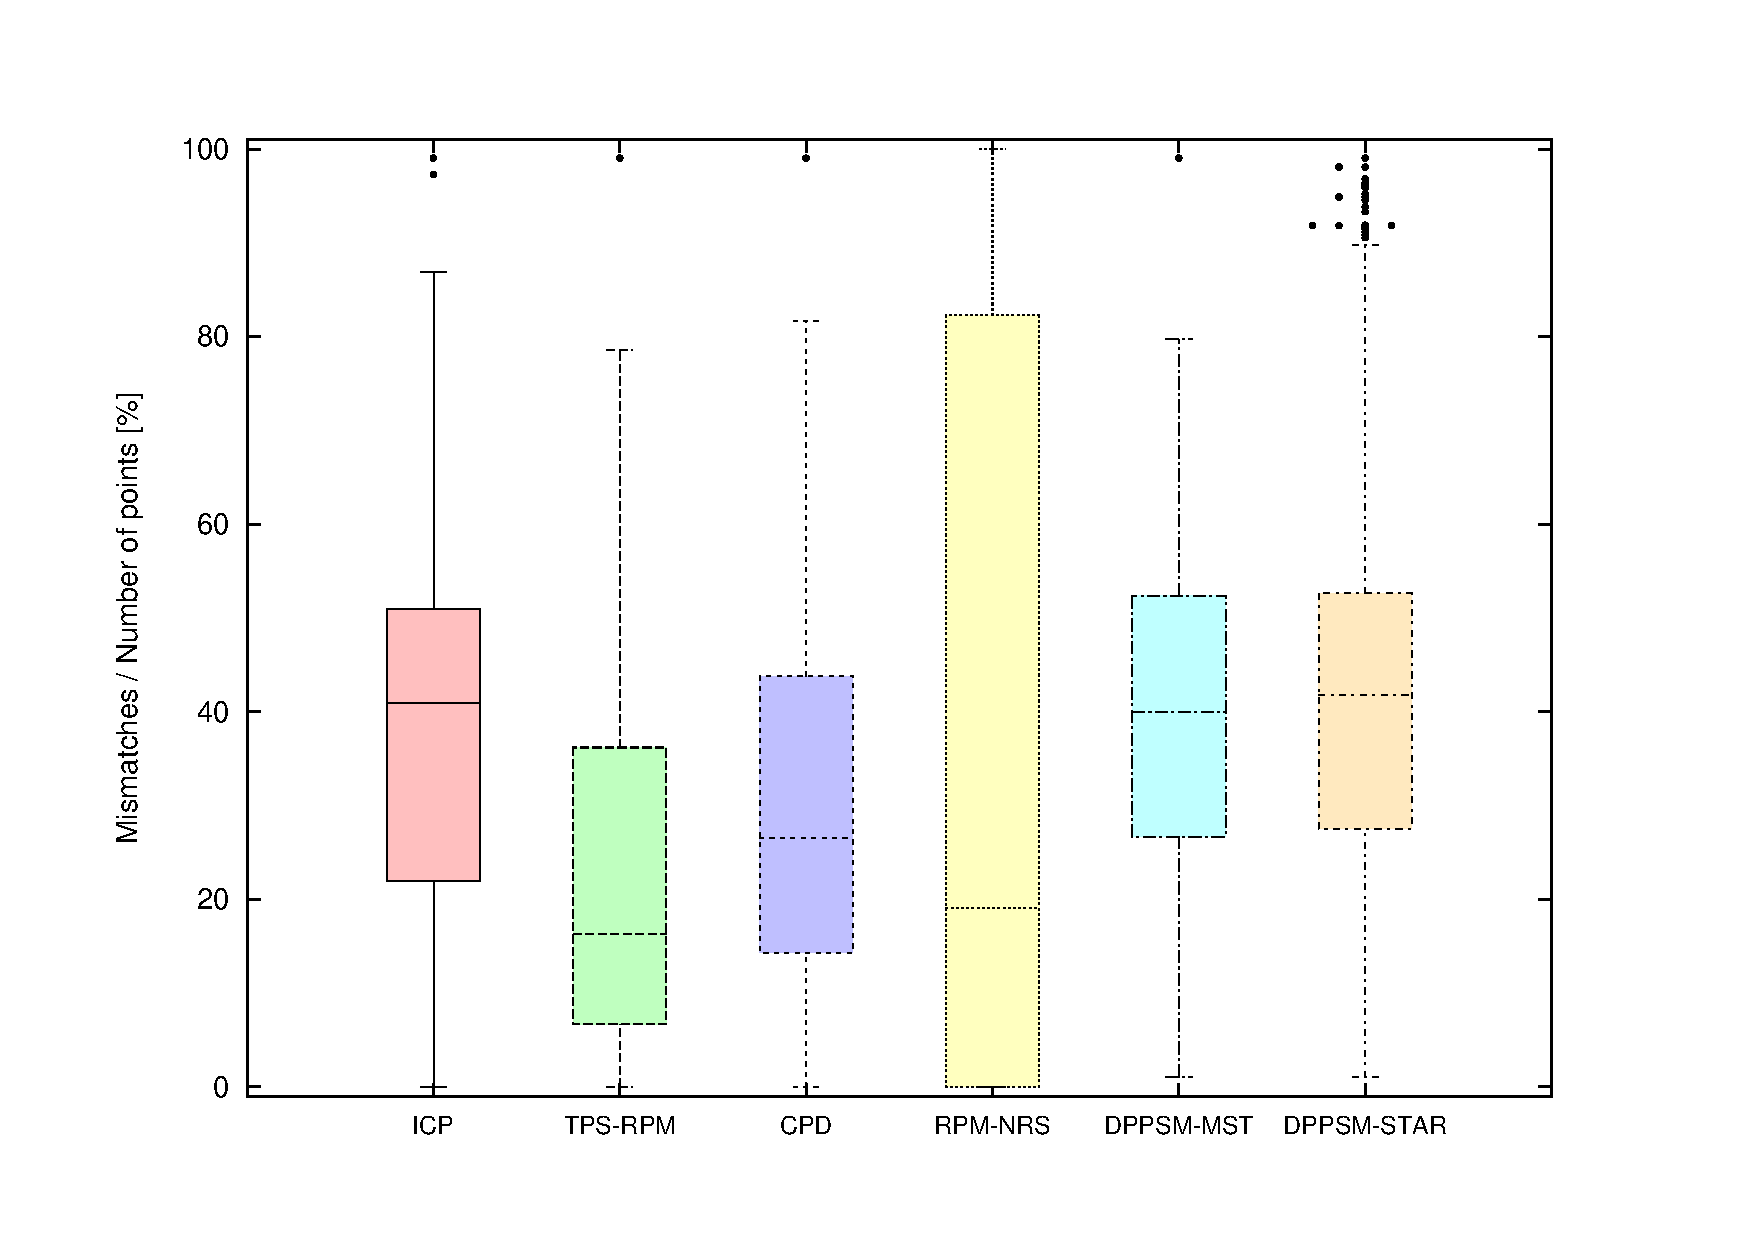
\includegraphics[width=\textwidth, trim=50 40 80 50,clip]{fig19.pdf}
                \caption{Mismatches}
                \label{fig:cp02_mismatchesChart}
        \end{subfigure}%
        
%         ~ %add desired spacing between images, e. g. ~, \quad, \qquad etc.
          %(or a blank line to force the subfigure onto a new line)
        \begin{subfigure}[b]{0.45\columnwidth}
                \centering
                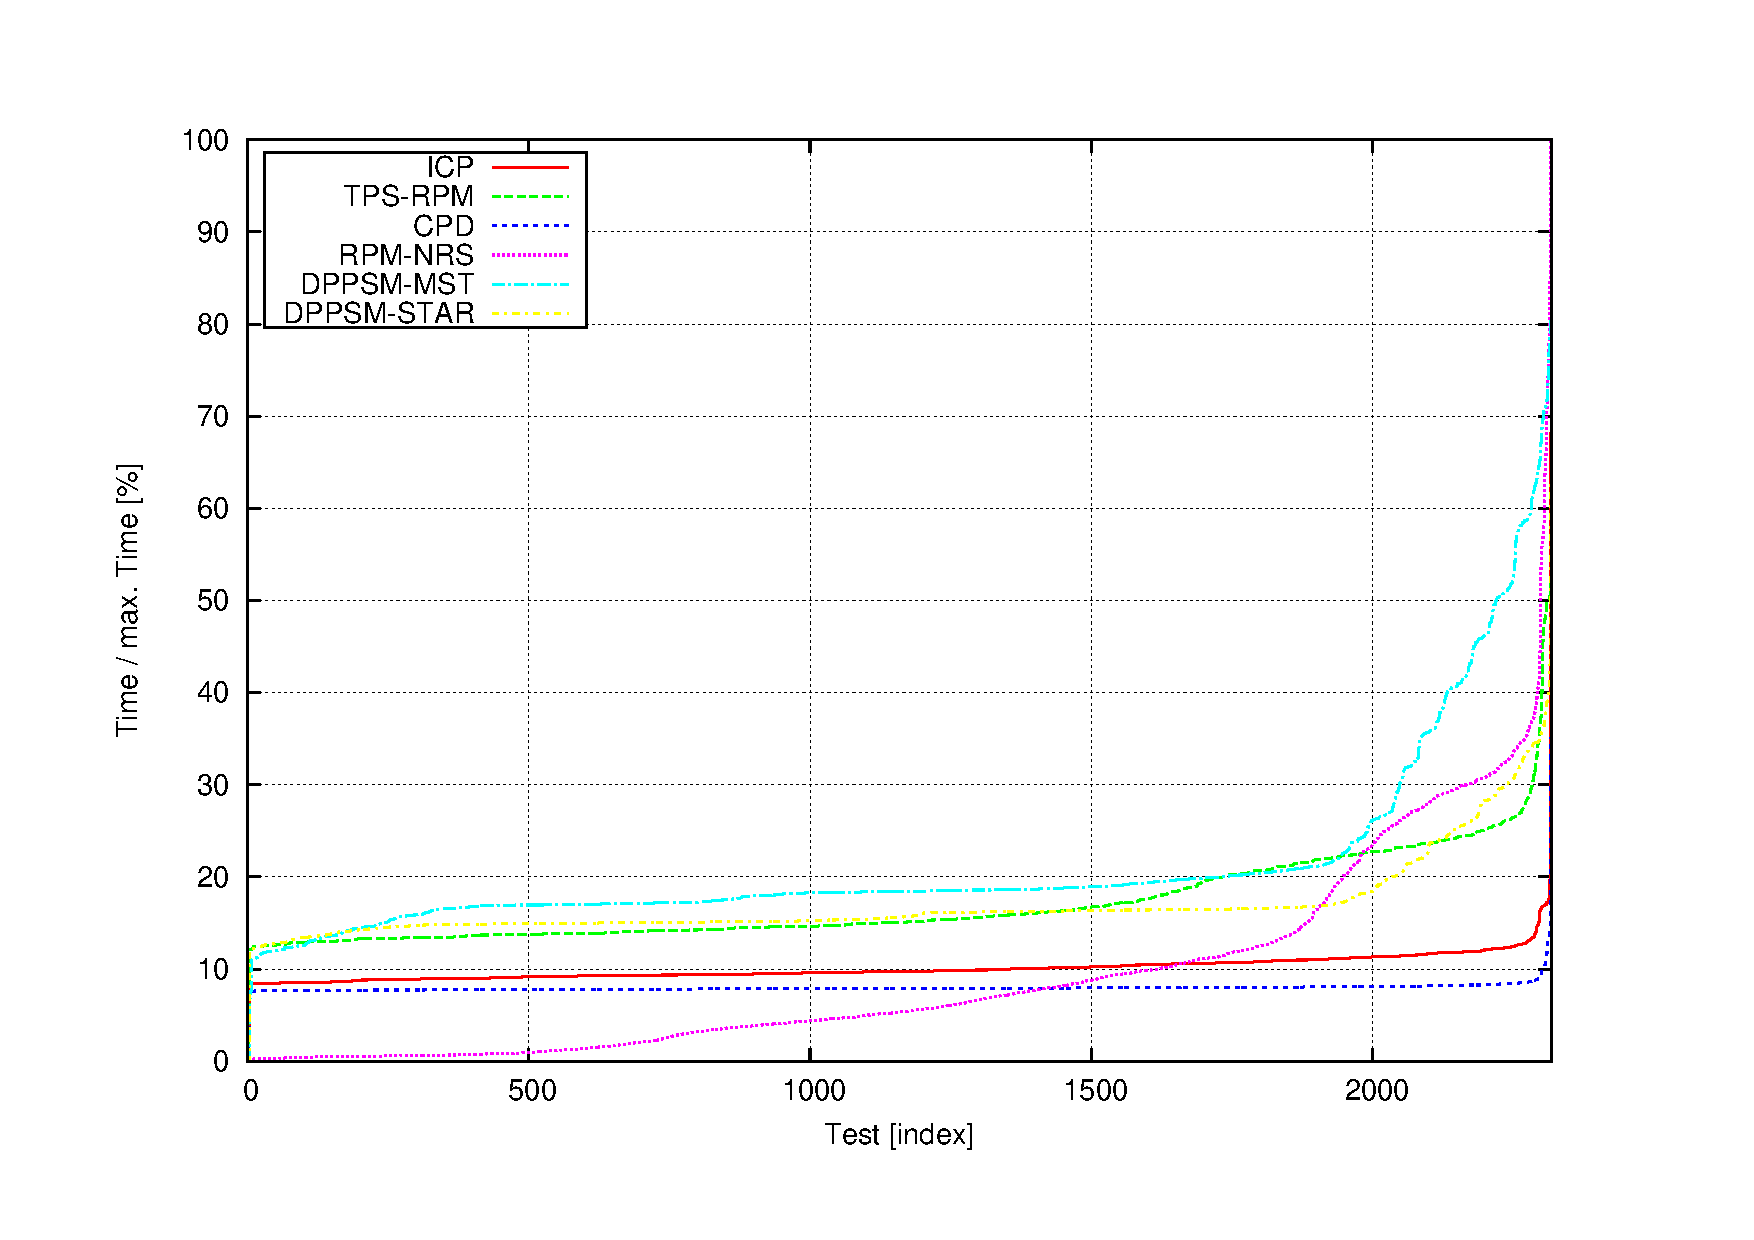
\includegraphics[width=\textwidth, trim=50 45 80 50,clip]{fig20.pdf}
                \caption{Times}
                \label{fig:cp02_timesChart}
        \end{subfigure}%

        \caption{Values obtained for nonrigid point set registration tested algorithms}\label{fig:cp02_chartsRegistration}
\end{figure*}

In the chart of figure \ref{fig:cp02_errorChart}, it is possible to see the error percentage made by each test. This 
error value is calculated as follows:

\begin{equation}\label{eq_errorCalculation}
error = { { \sqrt{ \sum_{i=1}^N \| p_i - t_{corresp(i)}\| } } \over N }
\end{equation}

where $N$ is the number of matched points (unmatched points are not considered), $corresp(i)$ is the index of the correspondence (in the ground truth dataset) for the point $i$ of the transformed model data set. $p$ and $t$ are points in the transformed model and ground truth datasets, respectively.
In the chart of figure \ref{fig:cp02_errorChart}, it is possible to notice that the best error rate is clearly found for the RPM-NRS 
algorithm, followed by the CPD.  The rest of algorithms present a similar behavior being, from the best to the 
worst, TPS-RPM, ICP, DPPSM-MST and DPPSM-STAR. The similarity between the last two algorithms is expectable, as the STAR is a simplification of MST in order to have a better time performance.

About the percentage of mismatches, in figure \ref{fig:cp02_mismatchesChart} it is possible to see the results obtained. In 
this chart, the percentage of mismatches is shown. The number of mismatches is calculated using a ground truth, and this 
percentage is obtained by dividing this value by the number of points in the smaller point set. The best algorithm in 
this case is TPS-RPM, followed again by CPD. However, RPM-RNS, which presented the best results in the previous test, 
has the worst results in this case. The relative behavior between ICP, DPPSM-MST and DPPSM-STAR in this test is 
similar to that obtained in the previous one.

Finally, in figure \ref{fig:cp02_timesChart} it is possible to see the relative time needed by each algorithm, with respect to 
the maximal time obtained in all the tests. This value is shown ordered. In this case, the more time consuming is 
DPPSM-MST. As expected, DPPSM-STAR is faster. The difference in efficiency shown in this chart demonstrates that worst 
results in the previous tests are compensated by a faster algorithm. RPM-NRS shows a high speed in some tests, but it is 
one of the slowest in the others. 

Analyzing data, it is due to the fact that the fastest results are obtained for clean 
tests, without outliers or noise. Once the noise and outliers increase, the algorithm becomes slower.
The most interesting behavior is that shown by the ICP and CPD algorithms, as they remain mostly constant. This is a good 
property to be exploited by our application, as it means that the computing time of those algorithms is independent on the input data. In fact, this supports the position of the CPD developers \citep{myronenko2010point}, who claim that their algorithm is 
the only one able to work with large point sets.

In this case, the choice of the methodologies used for the final tests was easy, as CPD clearly showed to have the best balance 
between number of mismatches, error and time consumption.

\subsection{Final algorithm evaluation}\label{ch:chapter02_02_03}

In this section, the final method is evaluated. As we did not find datasets thought for the evaluation of applications like ours, we developed a method that allowed us to indirectly measure errors in the tracking process. This method is explained next. Based on it, an study of the best parameters to be used in the CPD algorithm is performed. Finally, we will compare our method with other approaches.

\subsubsection{Method evaluation methodology}\label{ch:chapter02_02_03_01}

In this section, we want to evaluate the performance of our application. The main problem is that as said there is not a 
database available in which there is ground truth information about the correspondences of the contours of objects in 
an scene along the time. Because of that, we had to create an indirect way to measure the performance of our method. This was done by recording a sequence in which a person moves each part of its body using a Microsoft 
Kinect \textregistered, and process it to obtain the skeleton using the method described in \cite{shotton2013real}, 
implemented in the OpenNI libraries\footnote{\url{http://www.openni.org/}}.

The idea is the following: for each frame at time $t$, we have an initial skeleton provided by the Kinect, which is used as the initial configuration. From this skeleton, we repeat the following process for each joint $s_i$ in the skeleton $S$:
\begin{itemize}
 \item First, we look for the joint nearest points in the contour of the silhouette. To do that, we create the set of points $\mathcal{D} = \{ x \in X \cup s_i \}$, and a Delaunay triangulation \citep{lingas1994linear} is applied to them, as shown in figure \ref{fig:cp02_err_measure_triangulation}. This triangulation can be thought also as a visibility graph in which we will select the subset of points $X' \subseteq X$ for which all the points in $X'$ have a connection with the joint $s_i$. This idea is represented in the left image of figure \ref{fig:cp02_err_measure_trilateration}. For each point in $X'$, we also obtain the set $D = \{ x'_k - s_i) | x'_k \in X' \} $.
 \item For each $x'_k \in X'$, we obtain the set of correspondences $Y' \subseteq Y$ at the new frame $t + 1$, 
obtained using the CPD algorithm. Using this new set and $D$, we can obtain the new position $s'_i$ by 
trilateration. As we are working in 2D, in this case we can separate the $x$ and $y$ components in order to have two 
separate linear problems for which we have one variable and more than one equations. For instance, we solve the following system of equations to obtain the value of $s'_i(x)$:
 
 \begin{equation}
  \left( \begin{array}{cc}
1 & x'_0 \\
\vdots & \vdots \\
1 & x'_k \\
\vdots & \vdots \\
1 & x'_K \end{array} \right)
  \left( \begin{array}{c}
s'_i(x) \\
1 \end{array} \right) = 
  \left( \begin{array}{cc}
d_0 \\
\vdots \\
d_k \\
\vdots \\
d_K \end{array} \right)
 \end{equation}
 
In this system of linear equations, $K$ is the number of points in $X'$. A similar process is performed for $s'_i(y)$. In 
figure \ref{fig:cp02_err_measure_trilateration} it is possible to see, in the left, an initial $s_i$ corresponding to the 
\textit{torso} joint and the relative point set $X'$ at frame $t$. In the right side, the generated $s'_i$ with the 
respective $Y'$ set is shown for the frame $t + 1$.
\end{itemize}

\begin{figure*}[t]
        \centering
        \begin{subfigure}[b]{0.45\textwidth}
                \centering
                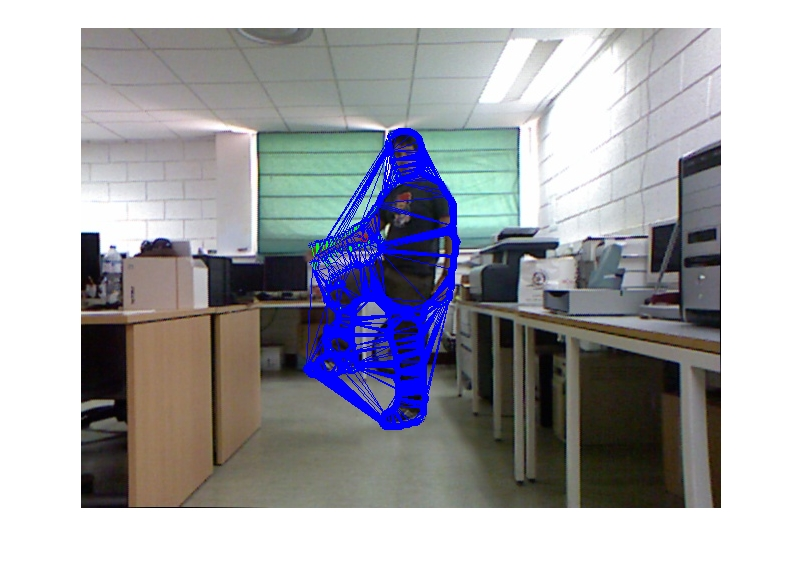
\includegraphics[width=\textwidth, trim=0 0 0 0,clip]{fig21.jpg}
                \caption{Triangulation}
                \label{fig:cp02_err_measure_triangulation}
        \end{subfigure}%
        ~
        \begin{subfigure}[b]{0.45\textwidth}
                \centering
                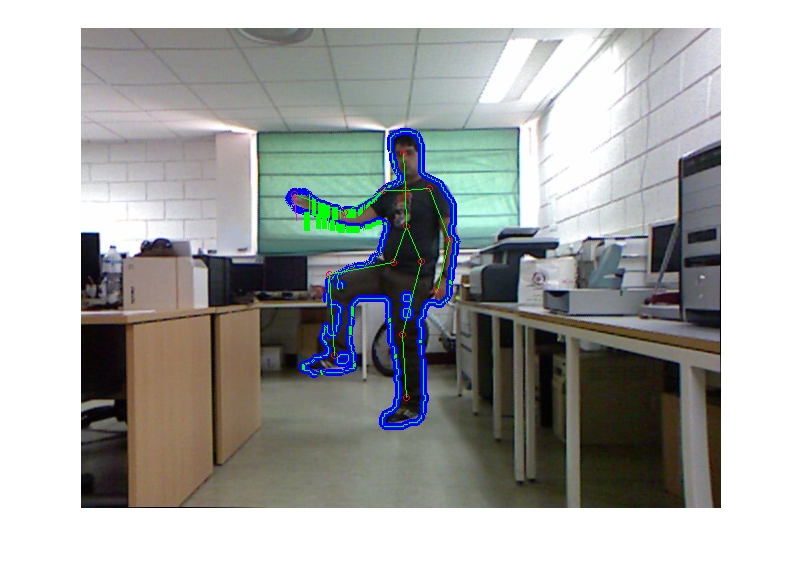
\includegraphics[width=\textwidth, trim=0 0 0 0,clip]{fig23.jpg}
                \caption{New joints obtained}
                \label{fig:cp02_err_measure_new_joints}
        \end{subfigure}%      
        
        \begin{subfigure}[b]{0.45\textwidth}
                \centering
                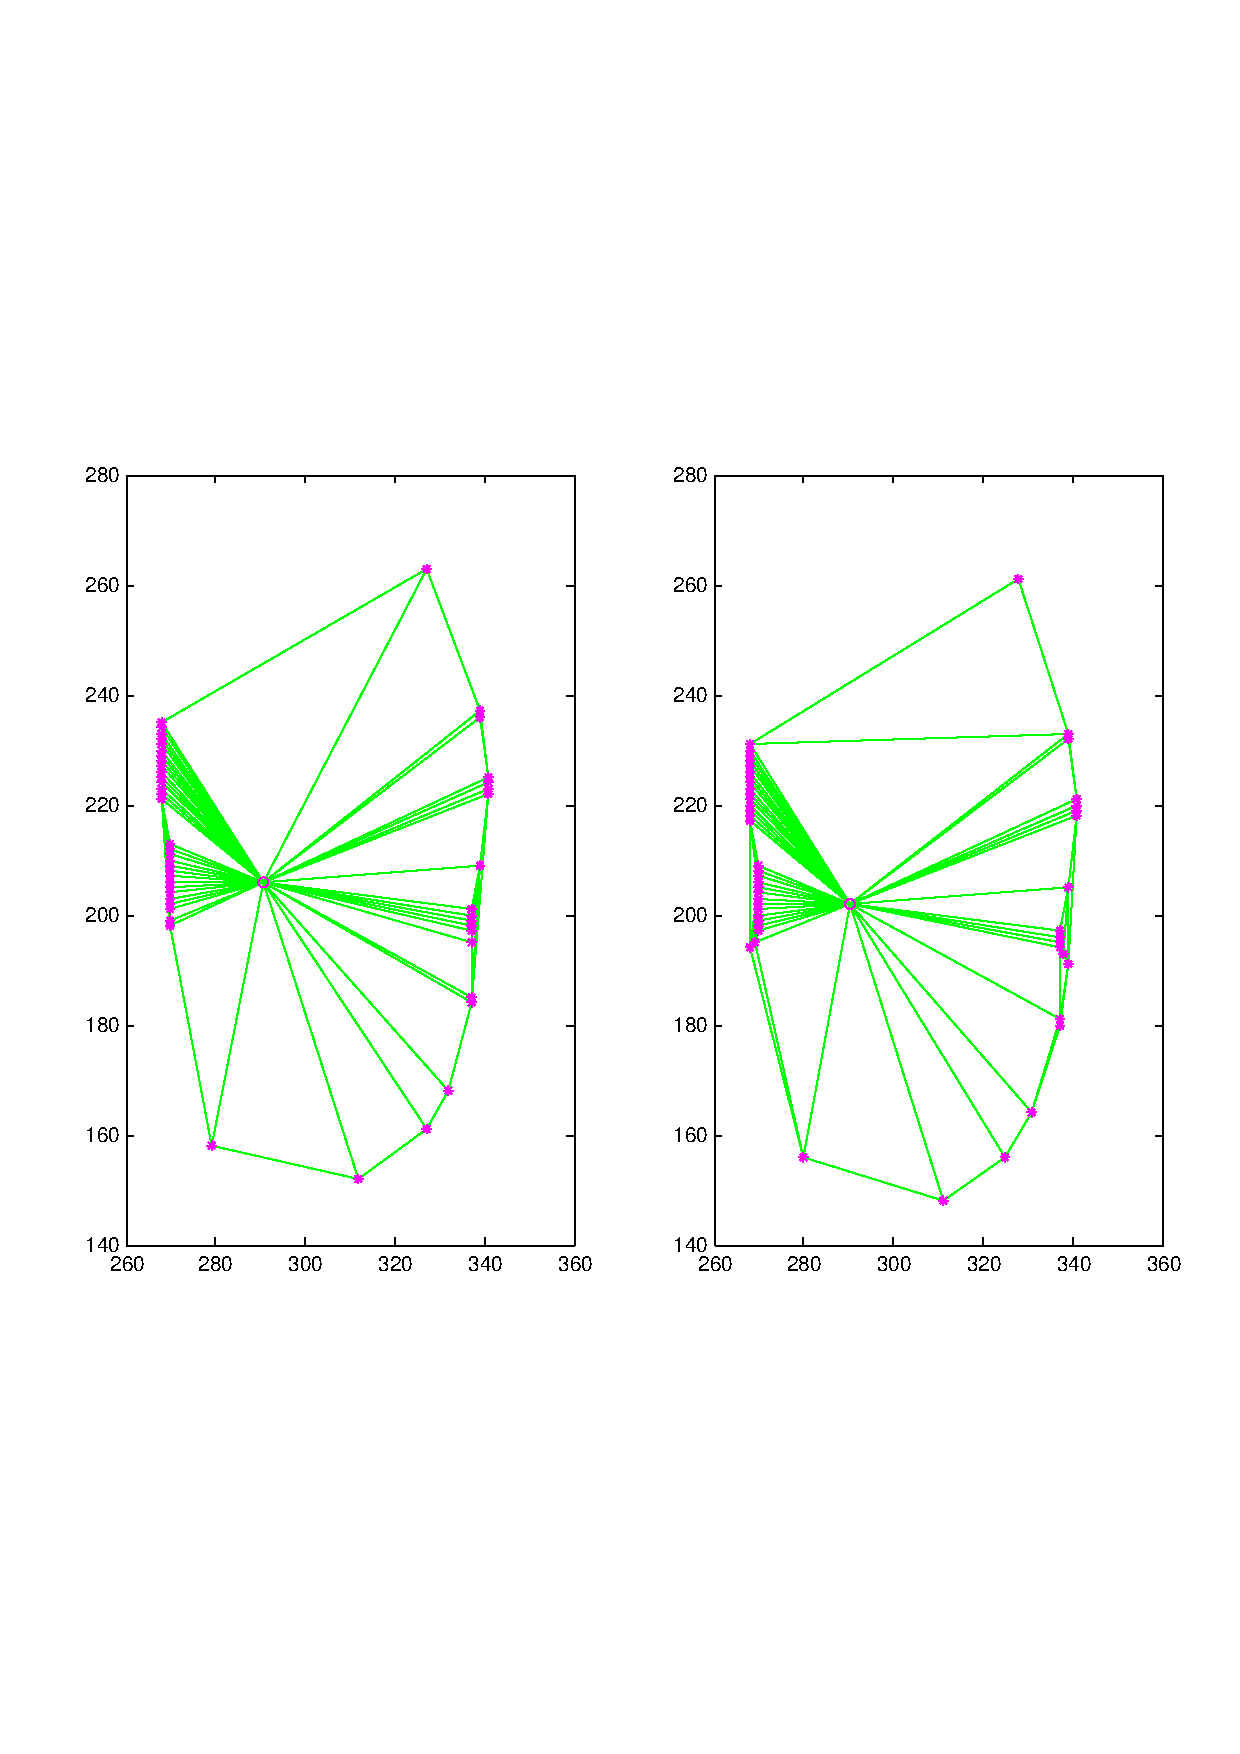
\includegraphics[width=\textwidth, trim=40 230 30 220,clip]{fig22.pdf}
                \caption{Trilateration}
                \label{fig:cp02_err_measure_trilateration}
        \end{subfigure}

        \caption{Skeleton generation process for the evaluation of the method}\label{fig:cp02_err_measure_skeleton}
\end{figure*}

The evaluation of the algorithm has been performed through the comparison of the position of each joint after doing the process 
described above in this section with the joint generated using the Kinect at each frame $t + 1$. Of course, using the Kinect as ground truth 
is not the best option as it has its own error. However, we think that if the behavior is similar using both 
approaches, we assume that the good performance of our algorithm is validated. To avoid including extra error, in each frame we start from 
the same joint set $S$, provided by the Kinect. That is, for the evaluation of the method, the initial skeleton is 
provided by the Kinect, so we just evaluate its evolution as generated by our application in the next frame. By doing so, we avoid the bias
produced by a deformation of the skeleton due to a single frame with bad matches. The measurement of the displacement is performed 
separately for each frame.
However, we think that, using the process described in this section with the trajectories obtained would allow to, 
given an initial set of joints, analyze its evolution along the time as Kinect does, but without the need of a previous 
model. So with some improvements, this method, which was presented as a indirect way for the evaluation of the application described in chapter \ref{ch:chapter02}, could be also used in motion analysis or virtual reality applications.

\subsubsection{Parameterization}\label{ch:chapter02_02_03_02}

In this section, we want to know which are the best tuning parameters for our application. In particular, we 
want to obtain the parameters that produce the best performance from the CPD, given the sort of data we are working 
with. Parameters chosen for this study are those that are described as free parameters in \cite{myronenko2010point}: 
$\omega$, $\lambda$ and $\beta$. According to the authors of the algorithm, parameter $\omega$, which can have a value 
between $0$ and $1$, reflects the assumption on the amount of noise in the point sets; parameter $\beta$ defines the 
width of the smoothing Gaussian filter used by the method; and $\lambda$ represents the trade off between the goodness 
of maximum likelihood fit and regularization.

For this evaluation, we measured the average distance between the joints generated with the method described in section \ref{ch:chapter02_02_03_01} and the Kinect joints used as ground truth. Results of this evaluation can be observed in figure \ref{fig:cp02_err_measure_parameterization}.

\begin{figure*}[t]
        \centering
        \begin{subfigure}[b]{0.45\textwidth}
                \centering
                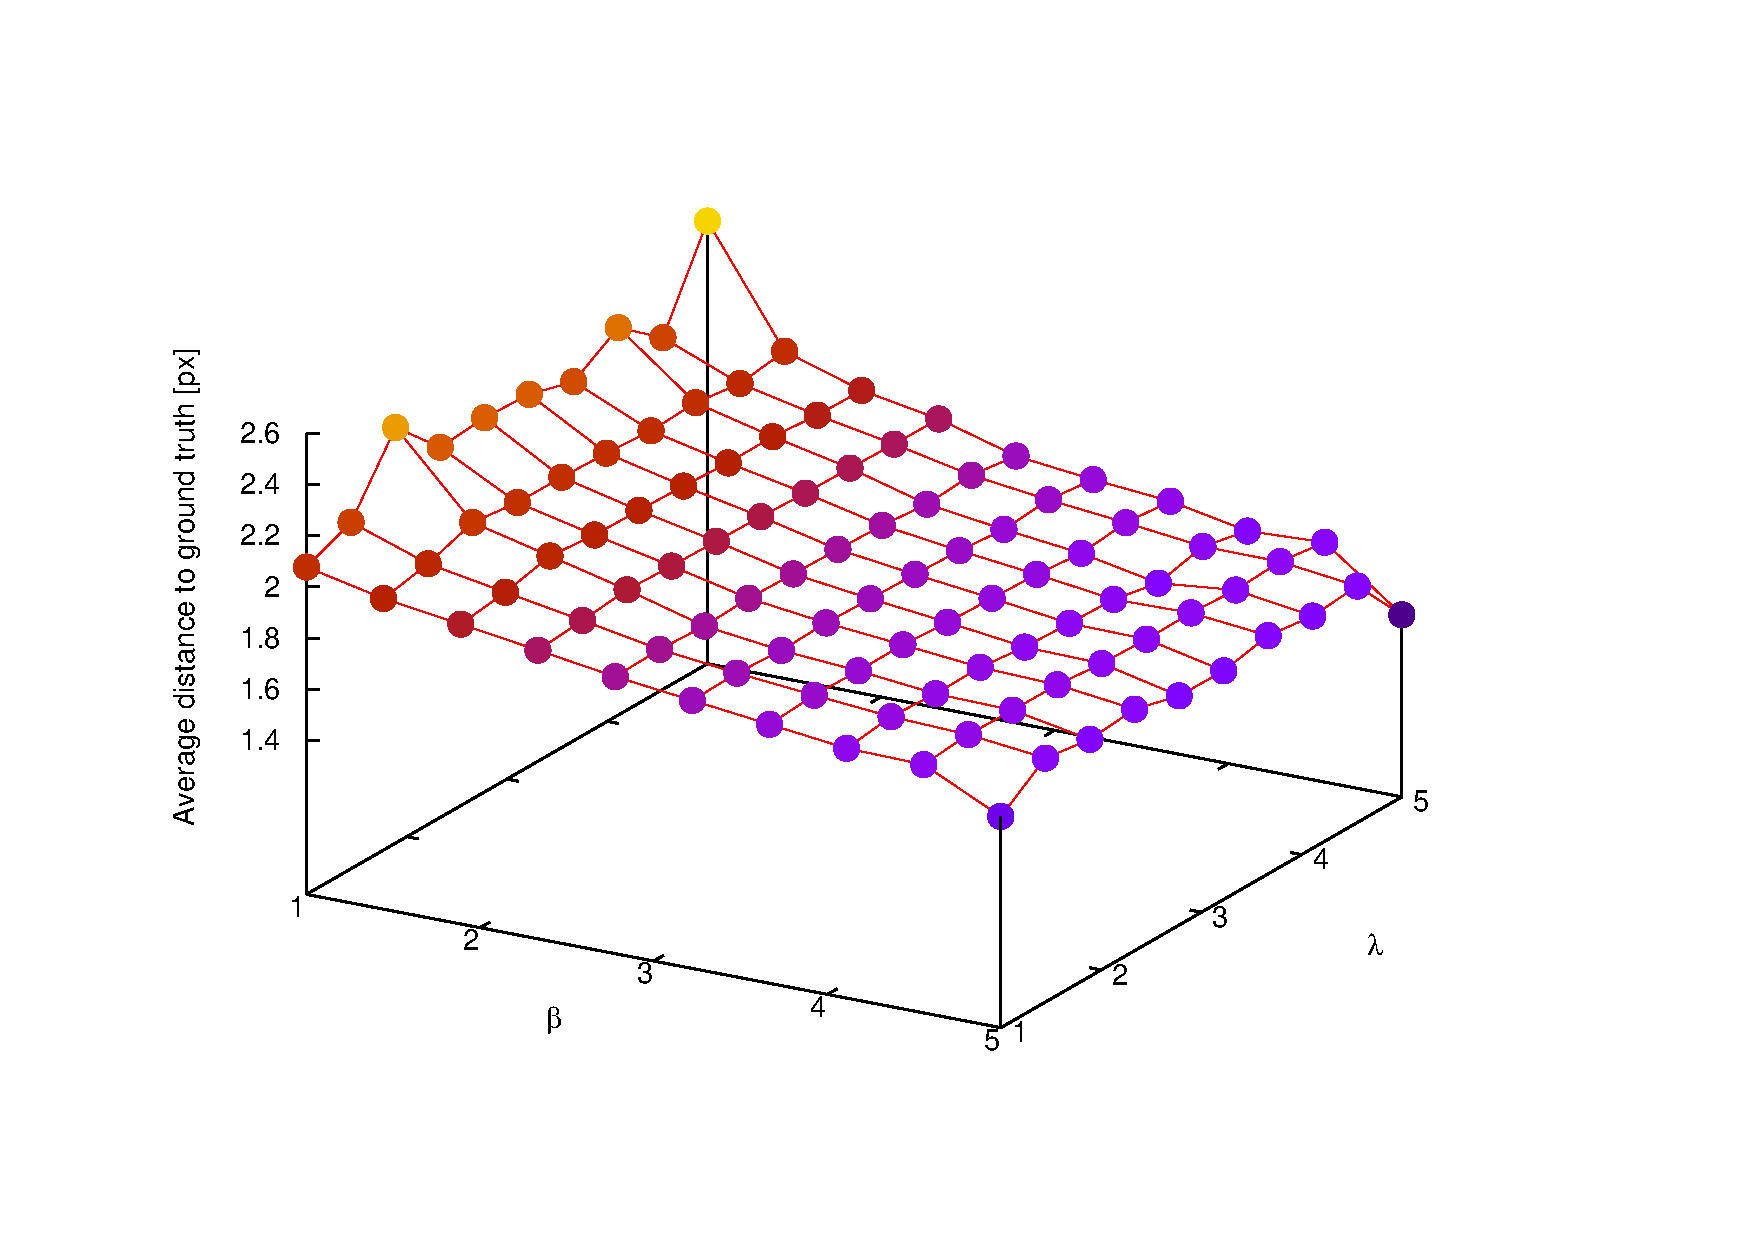
\includegraphics[width=\textwidth, trim=80 80 150 100,clip]{fig24.pdf}
                \caption{$\lambda$-$\beta$ comparison}
                \label{fig:cp02_err_measure_lambda_beta}
        \end{subfigure}%        
        ~ %add desired spacing between images, e. g. ~, \quad, \qquad etc.
          %(or a blank line to force the subfigure onto a new line)
        \begin{subfigure}[b]{0.45\textwidth}
                \centering
                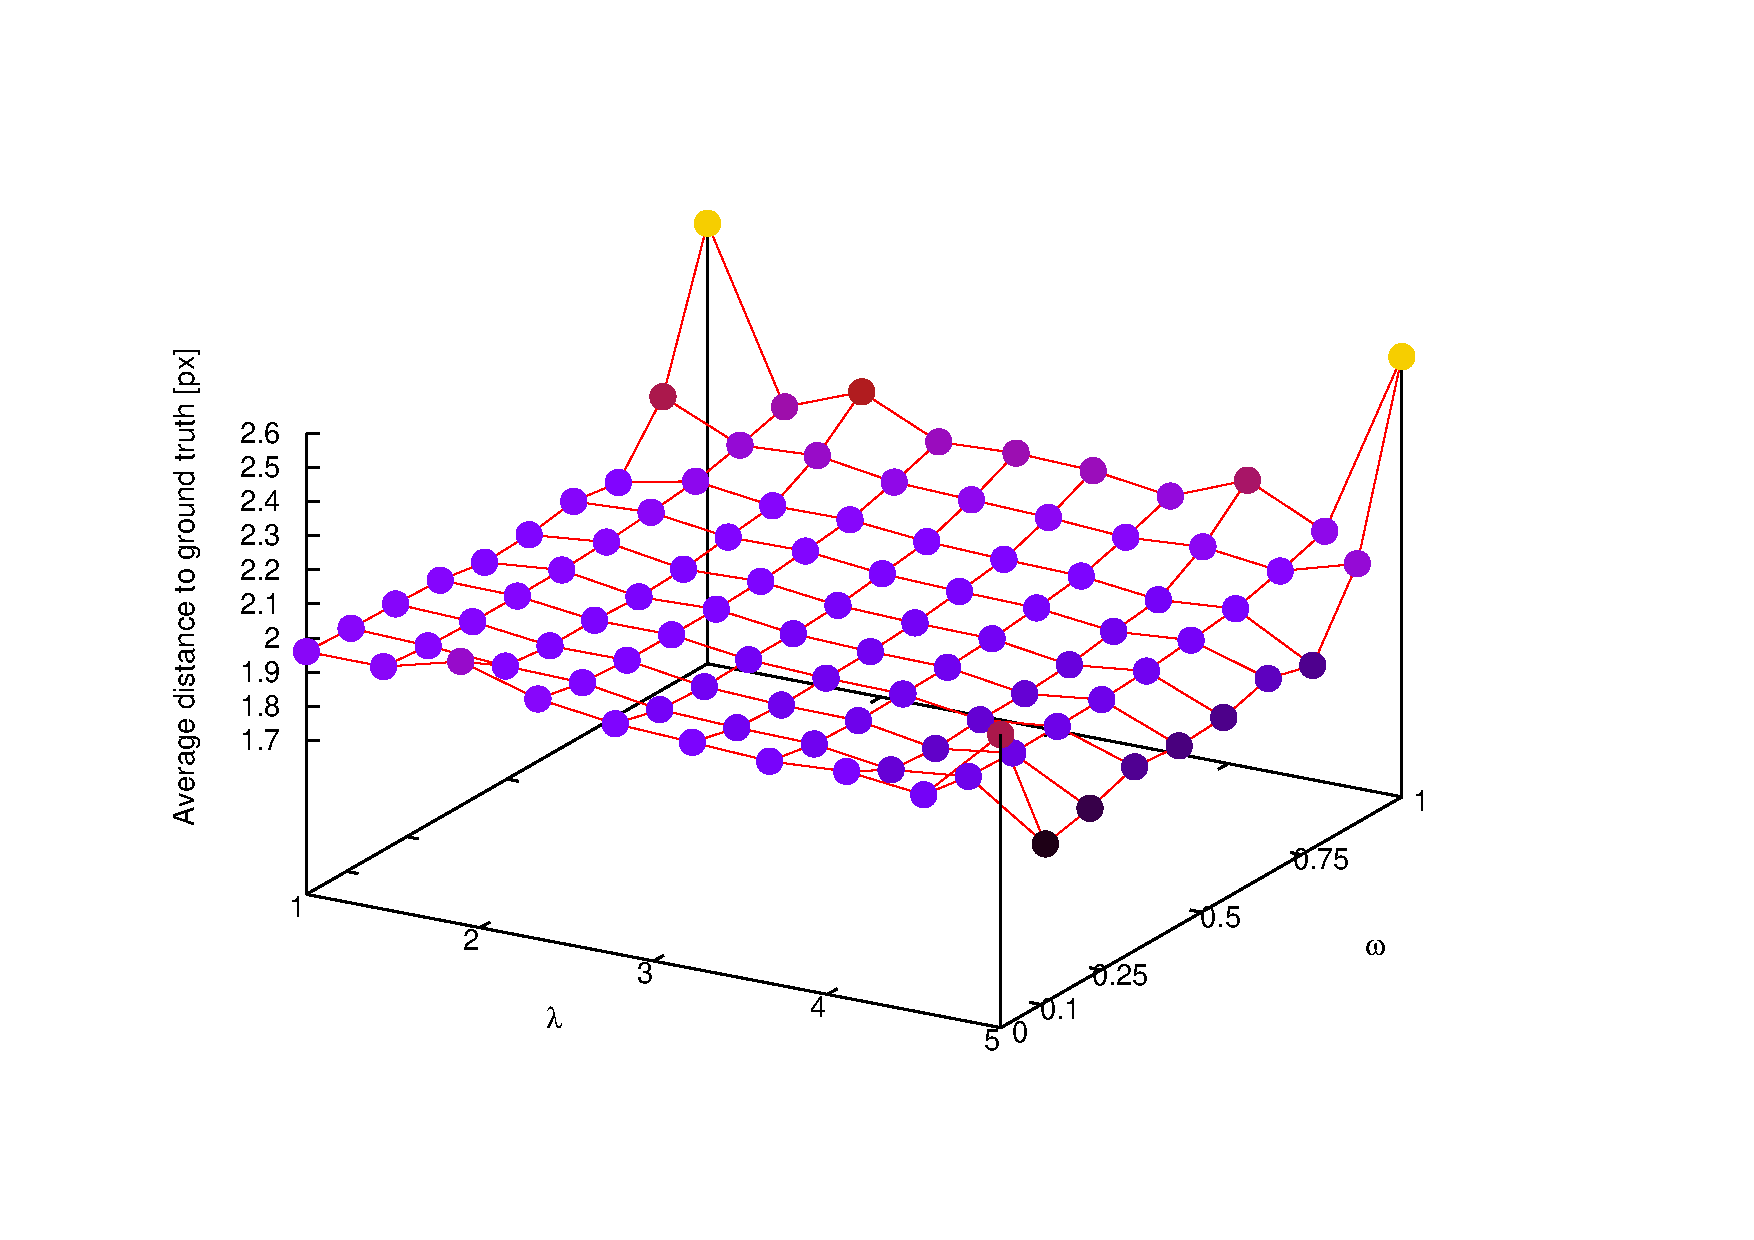
\includegraphics[width=\textwidth, trim=80 80 150 100,clip]{fig25.pdf}
                \caption{$\lambda$-$\omega$ comparison}
                \label{fig:cp02_err_measure_lambda_omega}
        \end{subfigure}
%         ~ %add desired spacing between images, e. g. ~, \quad, \qquad etc.
          %(or a blank line to force the subfigure onto a new line)
        \begin{subfigure}[b]{0.45\textwidth}
                \centering
                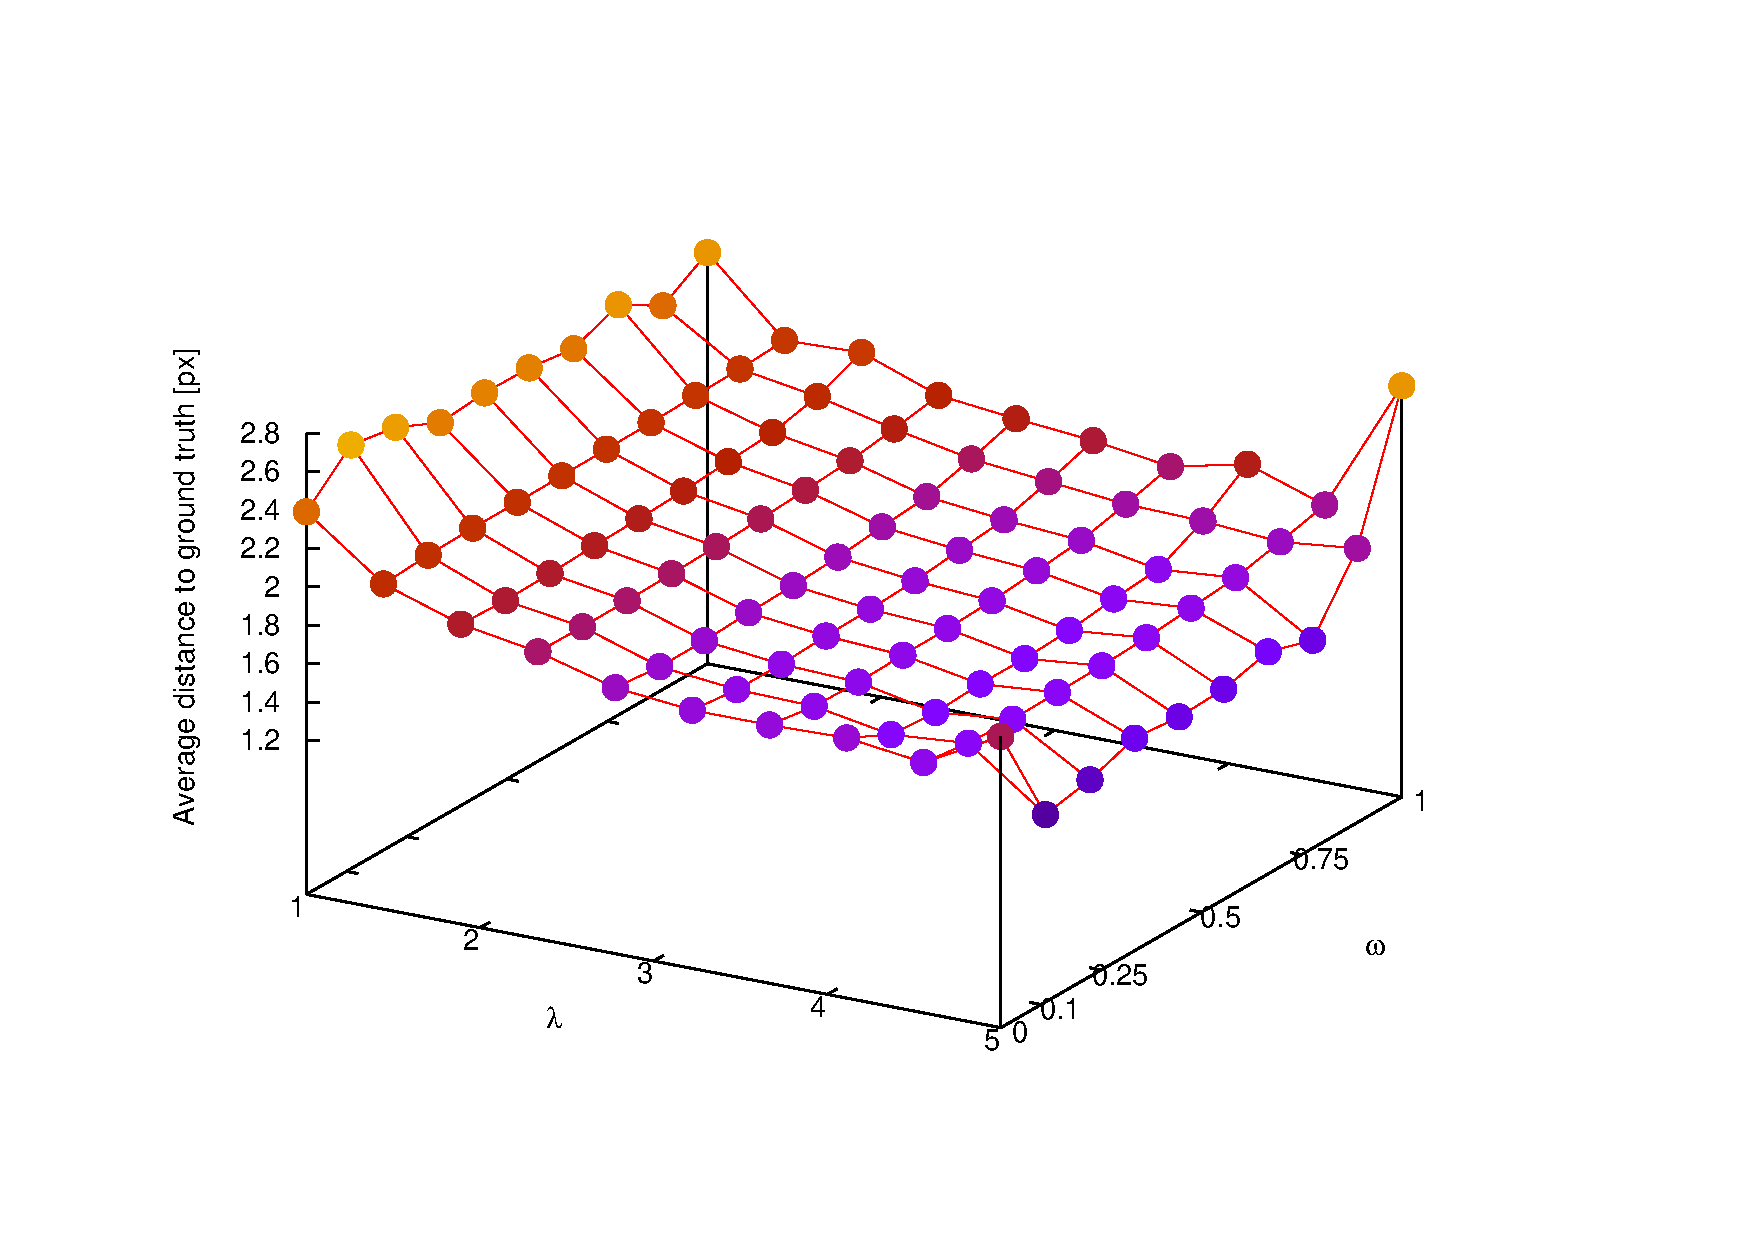
\includegraphics[width=\textwidth, trim=80 80 150 100,clip]{fig26.pdf}
                \caption{$\omega$-$\beta$ comparison}
                \label{fig:cp02_err_measure_omega_beta}
        \end{subfigure}%

        \caption{Comparison of the error obtained when combining different parameters.}\label{fig:cp02_err_measure_parameterization}
\end{figure*}

In this figure, best results are represented in dark blue, while worst are in yellow, representing high and low distances, 
respectively. From figure \ref{fig:cp02_err_measure_lambda_beta}, we deduced that best results are obtained when 
both $\lambda$ and $\beta$ are equal to $5$. It is important to evaluate both parameters together because, apart from 
the fact that both parameters are related to the smoothness regularization, the worst result is obtained precisely when 
$\lambda=5$, but $\beta=1$. In fact, it seems that the biggest contribution to the overall error is given by parameter 
$\beta$, except when its value is $1$. In this case, the contribution of $\lambda$ is uncertain.

The combination $\beta = 5$, $\lambda = 1$ is also a good choice, but if we have a look on figures \ref{fig:cp02_err_measure_lambda_omega} and \ref{fig:cp02_err_measure_omega_beta}, it is pretty clear that best results are obtained when $\beta=5$, $\lambda=5$, and $\omega=0.1$. This is quite surprising, as we assume that the error in the input data is quite high. However, worst results are obtained when $\omega=1$, with an average distance above 2.6\,pixels.

\subsubsection{Comparison with other methods}\label{ch:chapter02_02_03}

\begin{figure*}[t]
        \centering

        \begin{subfigure}[b]{0.5\columnwidth}
                \centering
                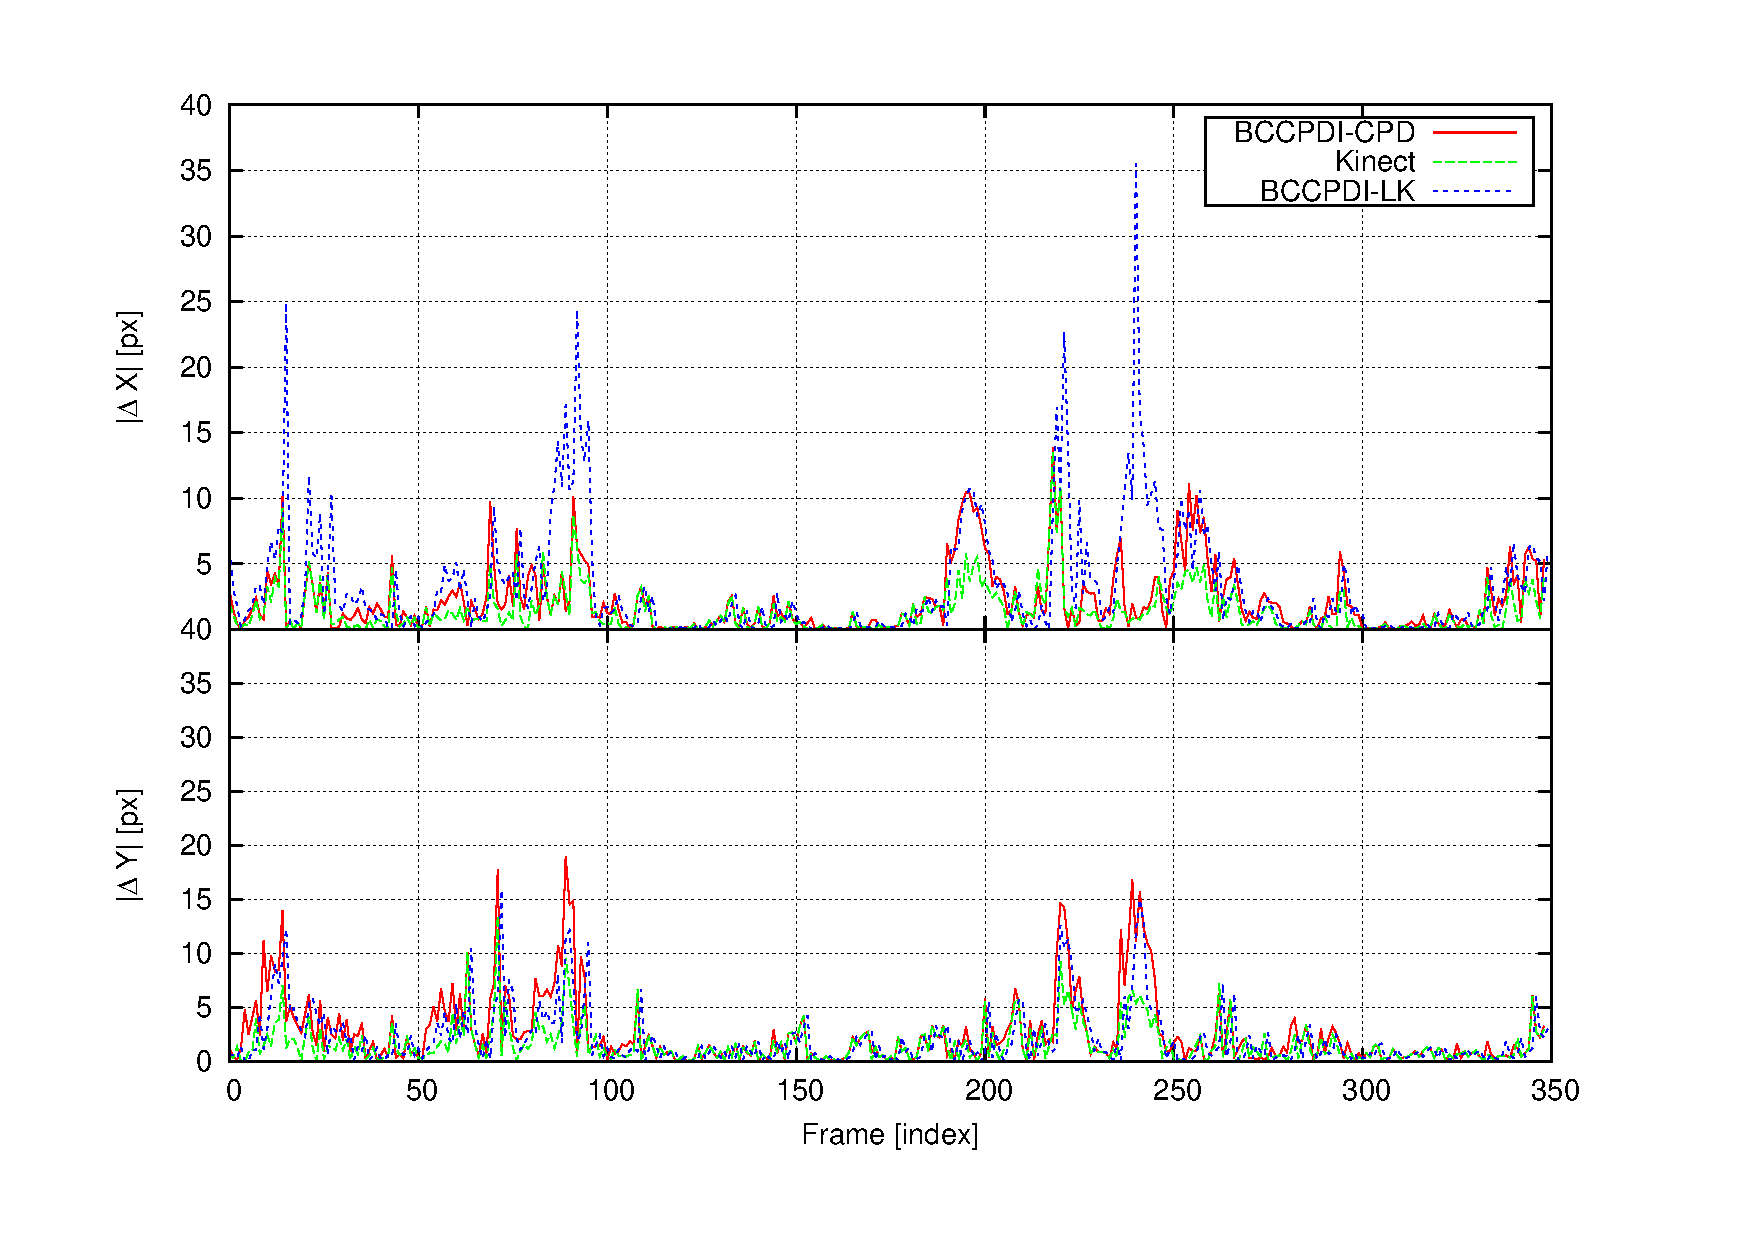
\includegraphics[width=\textwidth, trim=50 40 80 40,clip]{fig27.pdf}
                \caption{Left elbow}
                \label{fig:cp02_comparison_left_elbow}
        \end{subfigure}%        
        \begin{subfigure}[b]{0.5\columnwidth}
                \centering
		  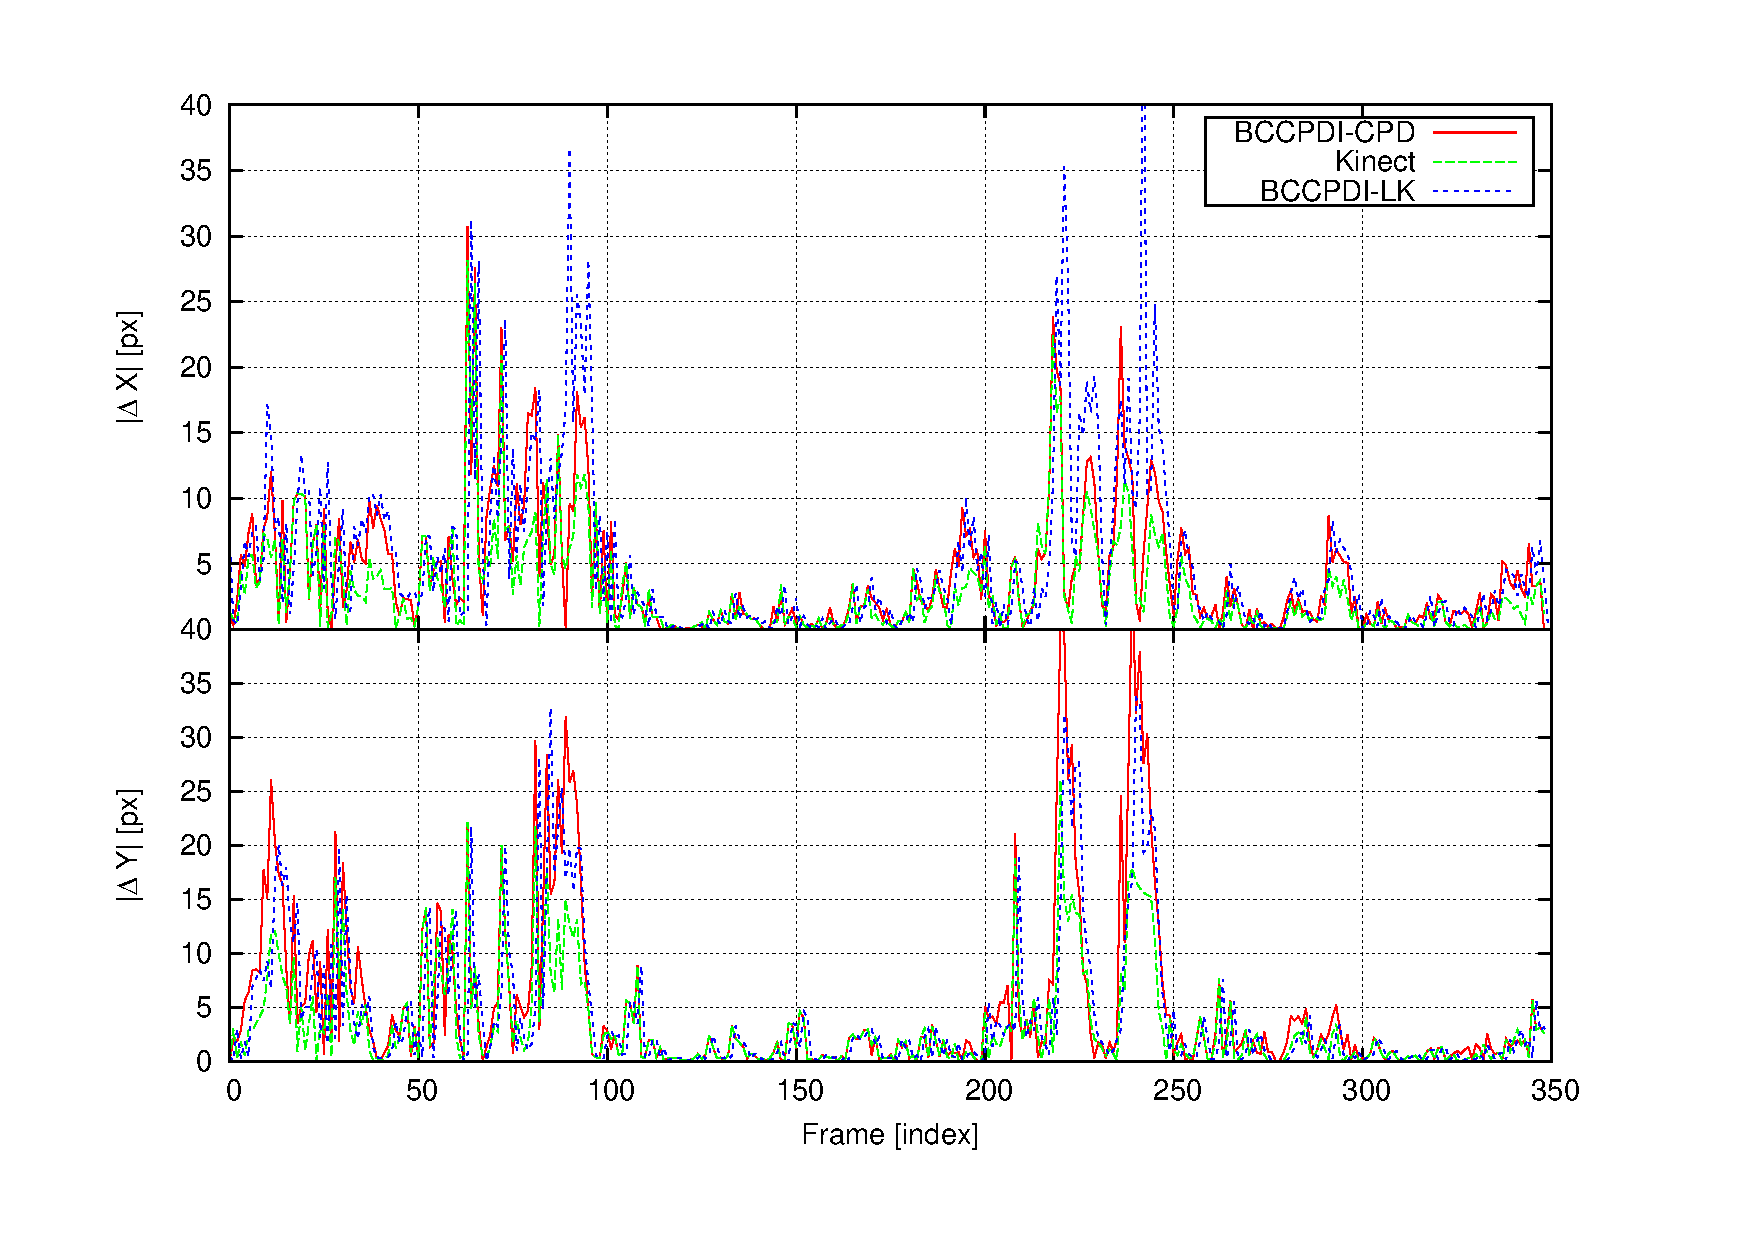
\includegraphics[width=\textwidth, trim=50 40 80 40,clip]{fig28.pdf}
                \caption{Left hand}
                \label{fig:cp02_comparison_left_hand}
        \end{subfigure}%        

        \begin{subfigure}[b]{0.5\columnwidth}
                \centering
                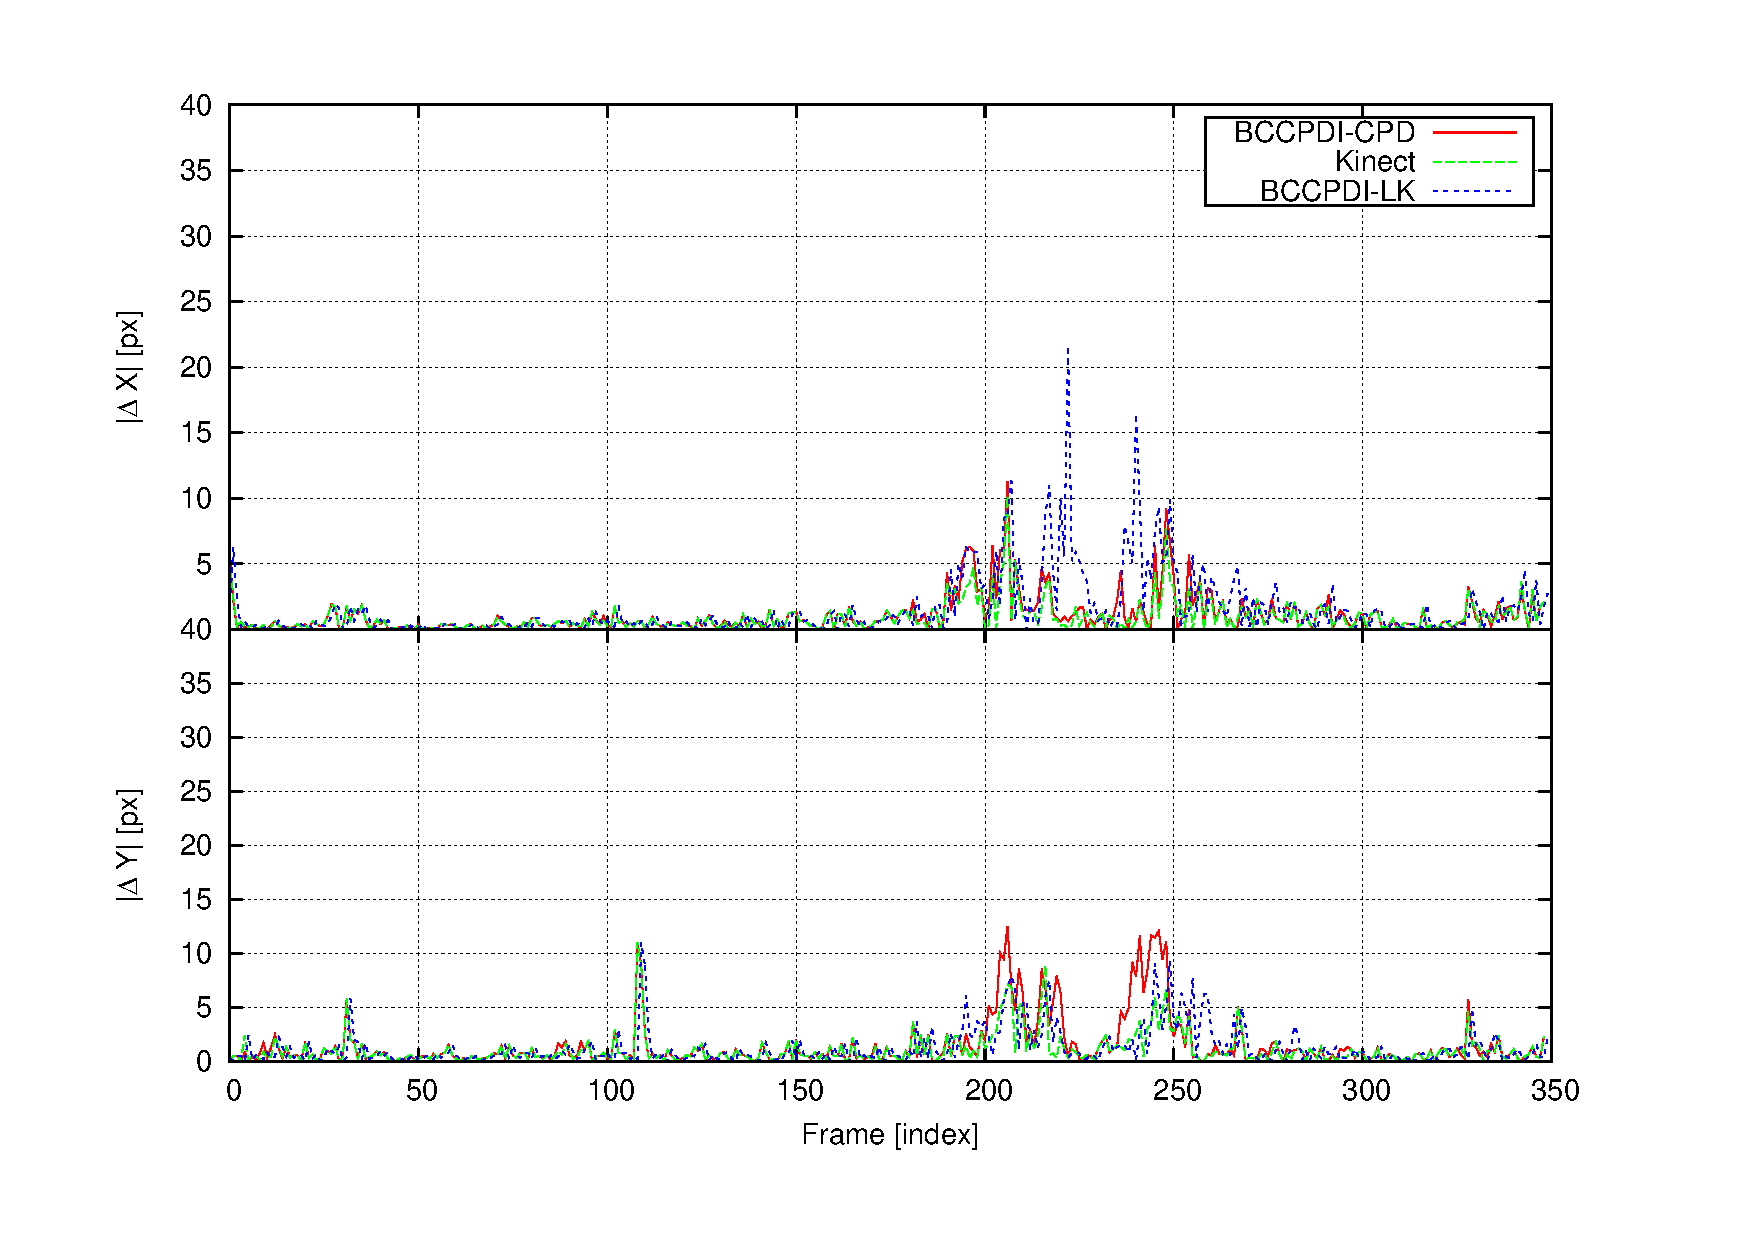
\includegraphics[width=\textwidth, trim=50 40 80 40,clip]{fig29.pdf}
                \caption{Left knee}
                \label{fig:cp02_comparison_left_knee}
        \end{subfigure}%        

        \caption{Comparison of the behavior in different joints.}\label{fig:cp02_comparison}
\end{figure*}

This is the first method that uses geometrical nonrigid point set 
registration methods to perform a contour tracking. One of the main contributions of our method is that we demonstrate 
that it is possible to perform such a task by using just geometrical information. Because of that, we compare our method 
with the output of the OpenNI algorithm that makes use of the Kinect, and with a simple Computer Vision based method. The 
former is considered as ground truth, because we have not found data which includes the information of 
the contour correspondences between frames at point level. 

However, as we will see, this method fails in certain circumstances. Due to that, we will pay attention to the frames in which the output of 
our algorithm and Kinect's diverge, in order to know what is happening. For the tests, we have calibrated the sensor in 
the way that the skeleton generated from the depth map obtained by the Kinect device is perfectly aligned with the $2D$ 
image obtained by its visible camera.

The Computer Vision based algorithm works as follows: starting from the set $X$, obtained with the method described in 
section \ref{ch:chapter02_01_01}, we apply the Lucas-Kanade \citep{bouguet2001pyramidal} optical flow 
method between the current and the next frame, obtaining the set $Y$. At this point, we have a set of correspondences 
equivalent to the set $\Phi$ described in section \ref{ch:chapter02_01_02_02}. Then, the process is similar to 
that described for our method.

In figure \ref{fig:cp02_comparison}, several charts show the behavior of our method compared with the other two, for three 
representative joints. In each of them, the absolute increment is shown separately for $x$ and $y$ coordinates in the 
upper and lower rows. The variations of these increments are shown along the frames. In these charts, BCCPDI-CPD is 
our method, BCCPDI-LK is the optical flow based method, and Kinect is the OpenNI output. The sequence, which is shown in 
the video available at \url{http://youtu.be/ZXSqKC07xJE}, consists on a person who moves separately each part of 
his body. The detection of this movement is reflected in the charts. For example, left arm is moved up and down between 
frames $0$ and $100$, and again between frames $200$ and $300$, as deduced by the bigger changes shown in the charts of 
figures \ref{fig:cp02_comparison_left_elbow} and \ref{fig:cp02_comparison_left_hand}. Left leg is also moved between frames $200$ 
and $250$, as seen in the chart of figure \ref{fig:cp02_comparison_left_knee}.

In the charts, we can see that the behavior of our method is quite similar to that shown by the Kinect. In fact, results are better than those shown by the Lucas-Kanade based method. In instance, if we take a look on the set of 
frames between $80$ and $100$ of the $|\Delta X|$ chart of figure \ref{fig:cp02_comparison_left_elbow}, they have a much 
bigger increment than that shown by the other two methods. 

If we look at frame $96$, (shown in figure \ref{fig:cp02_comparison_oflow_fails_elbow_lk_side}), we can observe how BCCPDI-LK fails in finding the correspondences, as 
the movement of the arm is mostly up to down. In this figure, correspondences are represented with a green line joining 
them, where the blue dots represent the points of the set $Y$ for which a correspondence was found. Joints are represented by the red circles, and in magenta 
we show the trajectory calculated for each of them. 

Also in figure 
\ref{fig:cp02_comparison_oflow_fails_elbow_lk_side} we can appreciate that the 
orientation of the correspondences is not the same for all of them, even when they belong to the same rigid part of the 
body. Likewise, if these results are compared with the tracking performed by the BCCPDI-CPD method, shown in figure 
\ref{fig:cp02_comparison_oflow_fails_elbow_cpd_side}, we can see that there are a lot of missing correspondences, specially 
in the upper side of the arm. A similar example is shown in figure \ref{fig:cp02_comparison_oflow_fails_knee_cpd_side} for 
the frame $226$, where we can see what is happening in the set of frames between $210$ and $230$, for which a 
different behavior is found for BCCCPDI-LK in figure \ref{fig:cp02_comparison_left_knee}. As happened in figure 
\ref{fig:cp02_comparison_oflow_fails_elbow_lk_side}, some correspondences are missing in the upper part of the thigh and some 
others are mismatches.

If we have a look at the upper chart in figure \ref{fig:cp02_comparison_left_elbow}, there is a set of frames in which the 
absolute increment of $x$ between frames is similar for BCCPDI-CPD and BCCPDI-LK. As said, Kinect is not perfect and 
there are some situations in which our method gives better results. This is one of these cases. 

In figure \ref{fig:cp02_comparison_kinect_fails} (frame $199$), we represent in blue the skeleton calculated by the 
Kinect method, and in green the skeleton generated by our method. In these frames, the person in the 
image was performing a lateral displacement. As can be seen, the skeleton provided by our method is better aligned with
the person than the obtained using the Kinect. 

\begin{figure*}[t]
        \centering

        \begin{subfigure}[b]{0.45\textwidth}
                \centering
                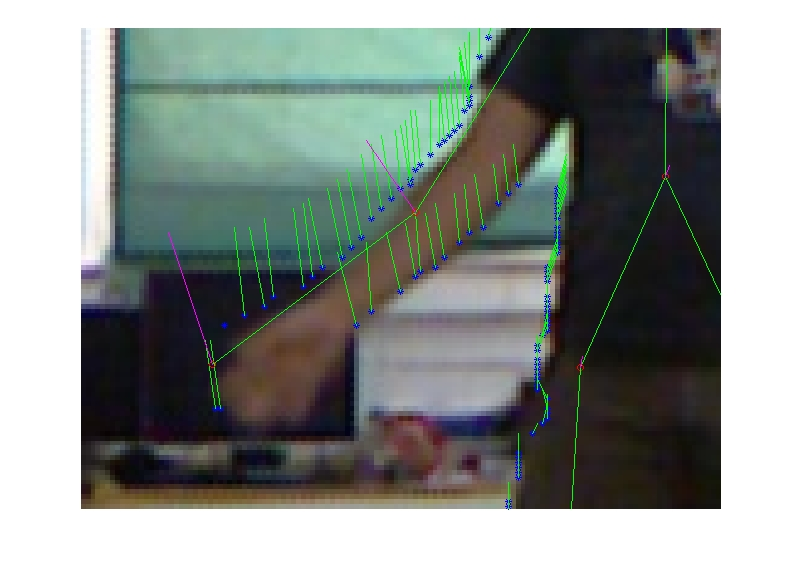
\includegraphics[width=\textwidth, trim=0 0 0 0,clip]{fig30.jpg}
                \caption{BCCPDI-CPD tracking, frame $96$.}
                \label{fig:cp02_comparison_oflow_fails_elbow_cpd_side}
        \end{subfigure}%        
	~
        \begin{subfigure}[b]{0.45\textwidth}
                \centering
                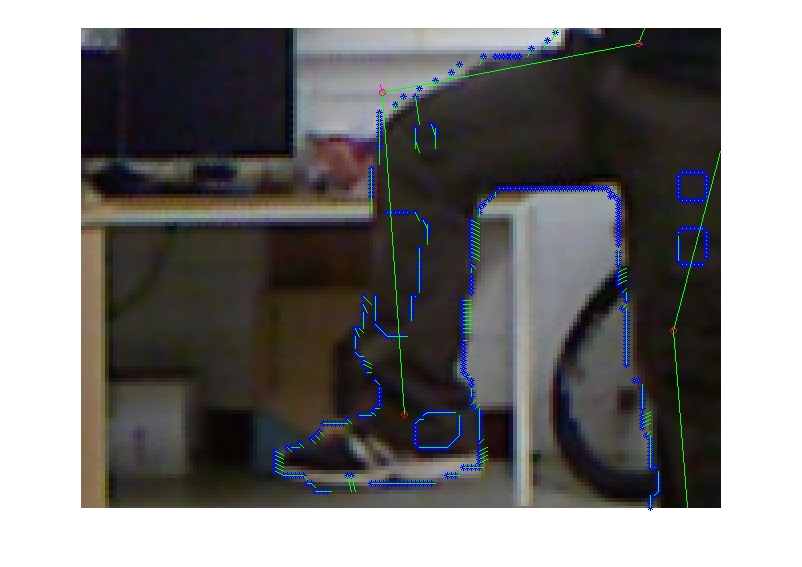
\includegraphics[width=\textwidth, trim=0 0 0 0,clip]{fig31.jpg}
                \caption{BCCPDI-CPD tracking, frame $226$.}
                \label{fig:cp02_comparison_oflow_fails_knee_cpd_side}
        \end{subfigure}%        

        \begin{subfigure}[b]{0.45\textwidth}
                \centering
                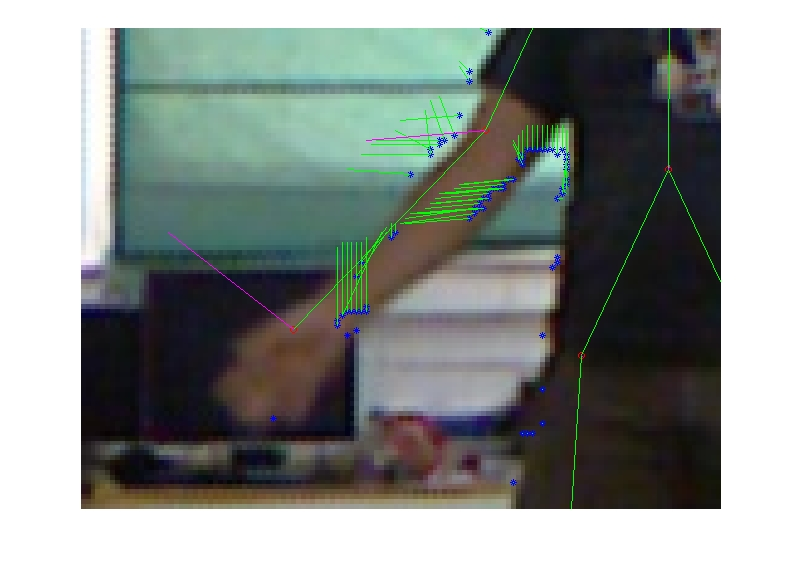
\includegraphics[width=\textwidth, trim=0 0 0 0,clip]{fig32.jpg}
                \caption{BCCPDI-LK tracking, frame $96$.}
                \label{fig:cp02_comparison_oflow_fails_elbow_lk_side}
        \end{subfigure}%    
        ~
        \begin{subfigure}[b]{0.45\textwidth}
                \centering
                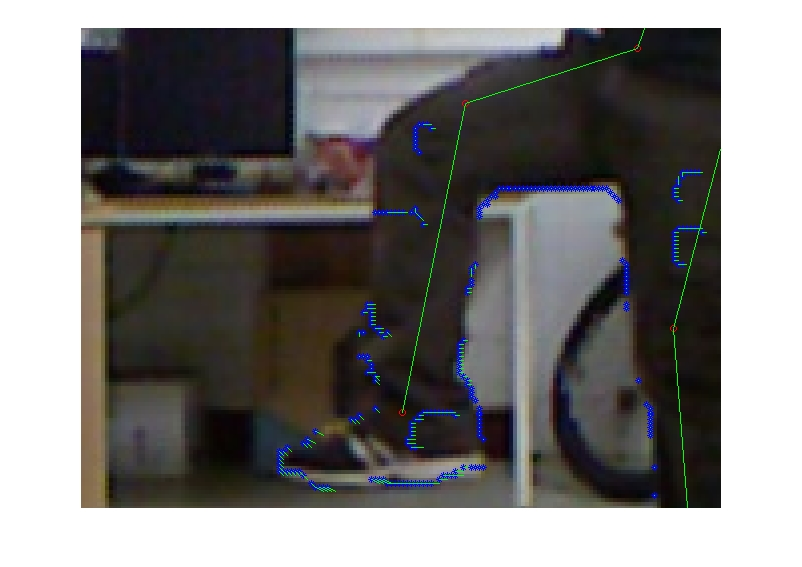
\includegraphics[width=\textwidth, trim=0 0 0 0,clip]{fig33.jpg}
                \caption{BCCPDI-LK tracking, frame $226$.}
                \label{fig:cp02_comparison_oflow_fails_knee_lk_side}
        \end{subfigure}%     

        \caption{Some frames in which BCCPDI-LK has a poor performance.}\label{fig:cp02_comparison}
\end{figure*}

\begin{figure*}[h]
  \centering
  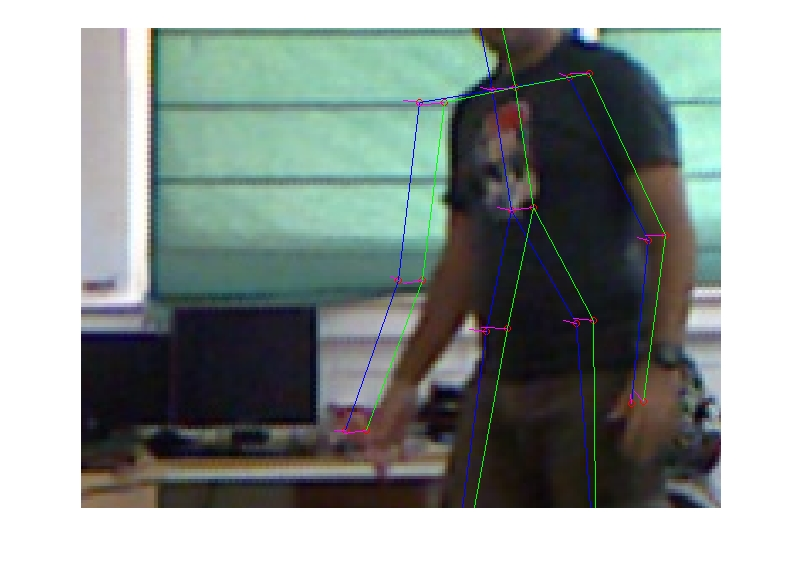
\includegraphics[width=0.5\columnwidth, trim=0 0 0 0,clip]{fig34.jpg}
  \caption{An example in which our method outperforms Kinect output.}
  \label{fig:cp02_comparison_kinect_fails}
\end{figure*}

In the video at \url{http://youtu.be/ZXSqKC07xJE} it is possible to see the full sequence and the output obtained by each different algorithm.

\FloatBarrier

\graphicspath{{./images/chapter03/bmps/}{./images/chapter03/vects/}{./images/chapter03/}}
\section{Evaluation of stereo 3D reconstruction algorithms}\label{ch:chapter03_04}

In this section, full performance graphs are presented showing the results obtained for the tests performed using the methods described in section \ref{ch:chapter03}. For the sake of brevity, the following notations will be used:
\begin{itemize}
 \item LGT – LIDAR-based ground truth evaluation (section \ref{ch:chapter03_01_01}).
 \item NFC – Number of false correspondences (section \ref{ch:chapter03_02}).
 \item NCC – Normalized cross correlation (section \ref{ch:chapter03_03}).
\end{itemize}

\subsection{Isolated filters}\label{ch:chapter03_04_01}

LGT evaluation results for each single filter presented in section \ref{ch:chapter03_03_03} are plotted in figure \ref{fig:cp03_isolated_LGT_bpp} and \ref{fig:cp03_isolated_LGT_avg}. Biggest improvements can be obtained through the use of the despeckle filter; the uniqueness constraint with a strict threshold is also quite effective at removing spurious values, albeit at the cost of a reduced density. Adaptive mean consistently reduces the average reconstruction error, even if on a relatively small scale (around 0.1\,px). At the level of sub-pixel error the gap filter produces worse results, which can be explained by the fact that the constant value interpolation that it performs is not accurate enough to capture pixel to pixel variations in the disparity values. Figure \ref{fig:cp03_isolated_NFC} shows the results for the NFC test: the despeckle and uniqueness filters still show clear improvements, as it does the adaptive mean, reinforcing the idea that their combined use is likely to boost the reconstruction performance. Results 
for 
the NCC test are plotted in figure \ref{fig:cp03_isolated_NCC}: unfortunately, the scores obtained from the different filters are almost overlapping. This behavior is not easily explained, although some factors are likely to contribute to it:
\begin{itemize}
 \item NCC scores are normalized with respect to the average image luminance, but local luminance variations still affect the resulting error value, so wrong reconstructions are not evenly weighted;
 \item the relatively small baseline in use reduces the measurable effects of reconstruction errors;
 \item the reconstruction quality is always quite good when using the algorithms described in section \ref{ch:chapter03_03} irrespective of the filters applied, and the test scores might be dominated by other error sources, such as the calibration.
\end{itemize}

\begin{figure*}[h!]
      \centering
      \begin{subfigure}[h]{\textwidth}
	\centering
	\includegraphics[width=\textwidth, height=0.5\textwidth, trim=0 0 0 0,clip]{filt_bpp}
	
	\caption{ Bad pixels percentage.}
	\label{fig:cp03_isolated_LGT_bpp} 
      \end{subfigure}%        
      
      \begin{subfigure}[h]{\textwidth}
	\centering
	\includegraphics[width=\textwidth, height=0.5\textwidth, trim=0 0 0 0,clip]{filt_avg}
	\caption{ Average error using LGT. }
	\label{fig:cp03_isolated_LGT_avg}
      \end{subfigure}%  
      \caption{ Isolated filters LGT performance. }
\end{figure*}

\begin{figure*}[h!]
  \centering
  \includegraphics[width=\textwidth, height=0.5\textwidth, trim=0 0 0 0,clip]{filt_nfc_perc}
  \caption{ Isolated filters NFC performance.}
  \label{fig:cp03_isolated_NFC}
\end{figure*}%        

\begin{figure*}[h!]
  \centering
  \includegraphics[width=\textwidth, height=0.5\textwidth, trim=0 0 0 0,clip]{filt_ncc}
  \caption{ Isolated filters NCC performance.}
  \label{fig:cp03_isolated_NCC}
\end{figure*}%  

\subsection{Composite filters}\label{ch:chapter03_04_02}

By combining different filters it is possible to obtain even better performances than when using them separately. Figure \ref{fig:cp03_composite_LGT_bpp}, \ref{fig:cp03_composite_LGT_avg} and \ref{fig:cp03_composite_LGT_dens} plot the results for the three Census-SGM configurations described in table \ref{table:cp03_algorithms} under the LGT test. Looking at the 90th percentile of figure \ref{fig:cp03_composite_LGT_bpp} it can be observed an improvement of around 6\% in the number of pixels exceeding the endpoint error for configurations 2 and 3; the average pixels error, instead, decreases by around 0.175\,px for the same two configurations (figure \ref{fig:cp03_composite_LGT_avg}). These improvements, however, come at the cost of a decreased disparity map density, as it is apparent in figure \ref{fig:cp03_composite_LGT_dens}: configuration 3, at the 90th percentile, has a density of around 58\%, while configuration 2 scores better, at about 65\%, which can still be considered acceptable for autonomous driving tasks; for comparison, the baseline 
method has a density close to 78\%, with 12\% bad pixels. Configurations 2 and 3 also produce the best results in the NFC test (figure \ref{fig:cp03_composite_NFC}), effectively reducing the number of wrong reconstructions falling within the vehicle trajectory to a negligible amount. The NCC test, instead, seems to indicate an opposite behavior across the tested configurations (figure \ref{fig:cp03_composite_NCC}), but as explained in section \ref{ch:chapter03_04_01} this data is likely to be very loosely related to the configuration in use.

\begin{figure*}[h!]
  \centering
  \begin{subfigure}[h]{\textwidth}
    \centering
    \includegraphics[width=\textwidth, height=0.5\textwidth, trim=0 0 0 0,clip]{comp_bpp}
    \caption{ Bad pixels percentage. }
    \label{fig:cp03_composite_LGT_bpp}
  \end{subfigure}%
  
  \begin{subfigure}[h]{\textwidth}
    \centering
    \includegraphics[width=\textwidth, height=0.5\textwidth, trim=0 0 0 0,clip]{comp_avg}
    \caption{ Average error. }
    \label{fig:cp03_composite_LGT_avg}
  \end{subfigure}%        
  \phantomcaption % new inserted command
\end{figure*}

\begin{figure*}[h!]
  \ContinuedFloat
  \begin{subfigure}[h]{\textwidth}
    \centering
    \includegraphics[width=\textwidth, height=0.5\textwidth, trim=0 0 0 0,clip]{comp_dens}
    \caption{ Output density. }
    \label{fig:cp03_composite_LGT_dens}
  \end{subfigure}%    
  \caption{ Composite filters LGT performance. }
\end{figure*}

\begin{figure*}[h!]
  \centering
  \includegraphics[width=\textwidth, height=0.5\textwidth, trim=0 0 0 0,clip]{comp_nfc_perc}
  \caption{ Composite filters NFC performance.}
  \label{fig:cp03_composite_NFC}
\end{figure*}%  

\begin{figure*}[h!]
  \centering
  \includegraphics[width=\textwidth, height=0.5\textwidth, trim=0 0 0 0,clip]{comp_ncc}
  \caption{ Composite filters NCC performance.}
  \label{fig:cp03_composite_NCC}
\end{figure*}%  

\begin{figure*}[h!]
  \centering
  \begin{subfigure}[h]{\textwidth}
    \centering
    \includegraphics[width=\textwidth, height=0.5\textwidth, trim=0 0 0 0,clip]{algo_bpp_ee3}
    \caption{ Bad pixels percentage. }
    \label{fig:cp03_algorithms_LGT_bpp}
  \end{subfigure}%        
  \phantomcaption % new inserted command
\end{figure*}

\begin{figure*}[h!]
  \ContinuedFloat
  \begin{subfigure}[h]{\textwidth}
    \centering
%       \framebox{\parbox{3in}{\centering \includegraphics[width=3in, trim=50 60 80 60,clip]{algo_avg_ee3}}}
    \includegraphics[width=\textwidth, height=0.5\textwidth, trim=0 0 0 0, clip]{algo_avg_ee3}
    \caption{ Average error. }
    \label{fig:cp03_algorithms_LGT_avg}
  \end{subfigure}%        

  \begin{subfigure}[h]{\textwidth}
    \centering
    \includegraphics[width=\textwidth, height=0.5\textwidth, trim=0 0 0 0,clip]{algo_dens_ee3}
    \caption{ Output density. }
    \label{fig:cp03_algorithms_LGT_dens}
  \end{subfigure}%    
  \caption{ Algorithms LGT performance. }
\end{figure*}

\begin{figure*}[h!]
  \centering
  \includegraphics[width=\textwidth, height=0.5\textwidth, trim=0 0 0 0,clip]{algo_nfc_perc}
  \caption{  Algorithms NFC performance.}
  \label{fig:cp03_algorithms_NFC}
\end{figure*}%  

\begin{figure*}[h!]
  \centering
  \includegraphics[width=\textwidth, height=0.5\textwidth, trim=0 0 0 0,clip]{algo_ncc}
  \caption{ Algorithms NCC performance.}
  \label{fig:cp03_algorithms_NCC}
\end{figure*}% 

\subsection{Algorithms comparison}\label{ch:chapter03_04_03}

Census-SGM configuration 2 has been selected as the best compromise between reconstruction quality and map density, and the following graphs illustrate its performance compared to that of the other two approaches described in section \ref{ch:chapter03_03}. LGT evaluation (figure \ref{fig:cp03_algorithms_LGT_bpp}, \ref{fig:cp03_algorithms_LGT_avg}, and \ref{fig:cp03_algorithms_LGT_dens}) shows that the bad pixel percentage is cut by around 7.5\% at the 90th percentile with respect to the baseline configuration, and by about 4.5\% if compared to the BT-SGM algorithm. The average error is also reduced by 0.15\,px, when using Census-SGM configuration 2, making it in line with the values obtained by ELAS. The missing pixels percentage increases to around 35\%, which is 12\% more than the baseline setup; however, a substantial portion of the additional unreconstructed points is due to the improved error suppression capabilities of the algorithm, and as such is expected behavior.
NFC evaluation (figure \ref{fig:cp03_algorithms_NFC}) produces results which are in line with the one obtained with the LGT test, which means that Census-SGM configuration 2 is measurably and consistently better than the alternative approaches, and as such the winning algorithm in this comparison.
NCC scores for the ELAS and BT-SGM algorithms are quite close (figure \ref{fig:cp03_algorithms_NCC}), and better than the Census-SGM baseline configuration (as expected), but the placement of Census-SGM configuration 2 looks suspicious (i.e. worse than the Census-SGM baseline configuration). For this reason, data coming from this test will have to undergo further investigation before it can be trusted as a reliable indicator of an algorithm's performance.

\FloatBarrier

\graphicspath{{./images/chapter04/bmps/}{./images/chapter04/vects/}{./images/chapter04/}}
\section{Stixel world}\label{ch:chapter04_02}

In this section, we will show some evaluation results obtained after the evaluation of the method described in chapter \ref{ch:chapter04}. Evaluations have been focused into four different scopes: 

\begin{itemize}
 \item Quality of the clustering process.
 \item Accuracy of the depth obtained for the computed stixels compared to the object level results.
 \item Recall of the obtained tracks related to several conditions.
 \item Computation time.
\end{itemize}

In order to compare our results with those obtained by \cite{gunyel2012stixels} and \cite{benenson2011stixels}, we have used the \emph{Bahnhof} sequence \citep{ess2009robust}, which contains about 7400 obstacle annotations with height $\geq 40\,px$ on 999 stereo pairs, with an image resolution of $640 \times 480$ pixels and a frame rate of about 15 frames per second. All tests described in this section have been performed over this sequence.

\subsection{Clustering}\label{ch:chapter04_02_01}

In this test, we want to know if the obstacle detection method described in section \ref{ch:chapter04_01_04_01} is good enough. For that, we compared our detections with the real obstacles appearing in each current frame. In these tests, we have executed the method with and without performing the filtering process described in section \ref{ch:chapter04_01_04_01_02}, obtaining the results shown in figure \ref{fig:cp04_detection_rate}.

\begin{figure}[h!]
\centering
\includegraphics[width=\textwidth,height=0.5\textwidth,trim=50 40 80 60,clip]{detectionRate}
\caption{Obstacles detection rate achieved using our clustering method.}\label{fig:cp04_detection_rate}
\end{figure}

\begin{figure}[h!]
\begin{tabular}{cc}
\includegraphics[width=0.49\textwidth]{stixelsDetection}\label{fig:cp04_stixels_detection} &
\includegraphics[width=0.49\textwidth]{obstacleDetection}\label{fig:cp04_obstacle_detection}
\end{tabular}
\caption{Comparison of the stixels obtained trough the method of \cite{benenson2012pedestrian} and the clustering performed in our method.}\label{fig:cp04_clustering_comparison}
\end{figure}

There, we compare each recall value with the number of frames in the sequence falling below it. That is, the faster the plot grows, the better the results are. There, we can see that, for a recall value of 90\%, just a 40\% fall below this value for the case in which we are filtering the obstacles. Situation is different when objects are not filtered. For the same recall value, a 60\% of the frames in the sequence are below this value.

\begin{figure}[h!t!!!!]
\centering
\includegraphics[width=\textwidth,height=0.5\textwidth,trim=50 40 80 60,clip]{disparity}
\caption{Difference in disparity achieved for both our clustering method and the initial stixel reconstruction.}\label{fig:cp04_disparity_comparison}
\end{figure}

In figure \ref{fig:cp04_clustering_comparison}, we can see the projected 3d output of the detected stixels. In the left image, the original stixels are shown. As we can see, there is a lot of noise, specially between obstacles. We can see also that a lot of free areas are detected as objects. In the right image we show just the stixels falling inside an obstacle, with their depths restored after the clustering process.

\subsection{Stixel accuracy}\label{ch:chapter04_02_02}

In this section, we want to show the accuracy found in the depth computation for the stixels related to our reconstruction after the clustering. For that, we used a disparity map obtained using the \ac{ELAS} algorithm as ground truth. In figure \ref{fig:cp04_disparity_comparison}, we compare the disparity error of the reconstructed disparity map related to the percentage of frames below this error. Red line represents the stixels error. This grows faster than the error of the clustered obstacles. If we look at the $x-coordinates$, we can see that approximately a 95\% of the images have a disparity error below a 10\%, while this error is just found for a 60\% of the images when the reconstruction is made by just the original stixel computation.

\begin{figure*}[h!]
        \centering
        \begin{subfigure}[b]{0.29\textwidth}
	  \begin{tabular}{c}
	    \includegraphics[height=0.375\figuresheight]{elas}
	  \end{tabular}
	  \caption{ELAS}\label{fig:cp04_reconstruction_elas}
        \end{subfigure}% 
        ~~~
        \begin{subfigure}[b]{0.29\textwidth}
	  \begin{tabular}{c}
	    \includegraphics[height=0.375\figuresheight]{stixels}
	  \end{tabular}
	  \caption{Stixels}\label{fig:cp04_reconstruction_stixels}
        \end{subfigure}%       
        ~~~
        \begin{subfigure}[b]{0.29\textwidth}
	  \begin{tabular}{c}
	    \includegraphics[height=0.375\figuresheight]{objects}
	  \end{tabular}
	  \caption{Object clustering}\label{fig:cp04_reconstruction_objects}
        \end{subfigure}%    
        ~~~
        \begin{subfigure}[b]{0.29\textwidth}
% 	  \centering
	  \begin{tabular}{c}
	    \includegraphics[height=0.375\figuresheight]{colorscale_jet}
	  \end{tabular}
	  \caption*{}\label{fig:cp04_reconstruction_colorscale}
        \end{subfigure}% 
        \caption{Comparison of the disparities obtained for \ac{ELAS}, stixels and the reconstructed objects.}\label{fig:cp04_reconstruction}
\end{figure*}

In figure \ref{fig:cp04_reconstruction}, we show the disparity maps obtained with \ac{ELAS}, the original stixels from \cite{benenson2011stixels} and our clustered obstacles. These are represented by a color scale, which is shown in the right side of the images. In this scale, the lower disparities (further) are represented in red, while the highest disparities are represented in blue.

\subsection{Tracking}\label{ch:chapter04_02_03}

In this section, results obtained in our tracking evaluation tests are shown in terms of the recall measured related to two different criteria:

\begin{itemize}
 \item The behavior of the tracking after a few frames (that is, the track length achievable with a certain level of confidence).
 \item The performance obtained when the time between frames is increased. 
\end{itemize}

In our tests, we evaluated different configurations attending to the matching metrics and the method used. From the whole set of tests, we have selected the most representative, which are shown in table \ref{table:cp04_configurations_tested}.

\begin{table}[h]
\begin{center}
\begin{tabular}{|c|c|c|c|c|}
  \hline
 \multirow{2}{*}{Name} & \multicolumn{3}{ c| }{Cost factors} & \multirow{2}{*}{Tracking Method} \\ \cline{2-4}
 & $\alpha_{SAD}$ & $\alpha_{hist}$ & $\alpha_{height}$ &  \\
 \hline
 Conf. 1 & 1 & 0 & 0 & \cite{gunyel2012stixels} \\
 Conf. 2 & 0.5 & 0 & 0.5 & \cite{gunyel2012stixels} \\
 \hline
 Conf. 3 & 1 & 0 & 0 & Two-level tracking \\
 Conf. 4 & 0.5 & 0 & 0.5 & Two-level tracking \\
 Conf. 5 & 0 & 1 & 0 & Two-level tracking \\
 Conf. 6 & 0 & 0.5 & 0.5 & Two-level tracking \\
 \hline
 Conf. 7 & 0 & 0 & 0 & Object tracking \\
 \hline
\end{tabular}
\end{center}
\caption{Configurations for which the evaluation results are shown.}\label{table:cp04_configurations_tested}
\end{table}

Two of these configurations are from the implementation of the method by \cite{gunyel2012stixels}, available at \url{https://bitbucket.org/rodrigob/doppia}, with just the \ac{SAD} cost, and the final configuration described in their paper, in which $\alpha_{SAD} = 0.5$ and $\alpha_{height} = 0.5$, in order to know the real contribution of factor $\alpha_{height}$. Same process is done for the two-level tracking method, in which we evaluate also the contribution of factor $\alpha_{hist}$. Finally, we do a evaluation of the results obtained by using the object based tracking, without doing a previous stixel level tracking. As this level is not needed, $\alpha_{SAD} = \alpha_{hist} = \alpha_{height} = 0$.

\subsubsection{Performance along the sequence}\label{ch:chapter04_02_03_01}

For the evaluation of the tracking capabilities of the method, we followed the same strategy described in \cite{gunyel2012stixels}: we used annotated obstacle bounding boxes provided as ground truth with the evaluated sequence. Starting from ground truth annotations at a certain frame, each evaluated configuration is used to predict the bounding box positions up to \emph{$\Delta$ frames} in the future. For each frame, we evaluate the recall using the standard intersection over union metric. By running this evaluation starting from every frame in a video sequence we obtain the \emph{recall vs. $\Delta$ frames} curve shown at figure \ref{fig:cp04_recall_vs_delta_frames}, in which all the configurations are computed. 

\begin{figure}[h!]
\centering
\includegraphics[width=\textwidth,height=0.5\textwidth,trim=50 40 80 60,clip]{recall_vs_delta_frames}
\caption{Comparison of the recall obtained for the different configurations.}\label{fig:cp04_recall_vs_delta_frames}
\end{figure}

In this chart, we can see that the \cite{gunyel2012stixels} method falls quite fast, with a recall below 50\% just after 5 frames have passed. Also, the contribution of $\alpha_{height}$ is not clear. About the two-level tracking methods, results are better, specially those in which $\alpha_{hist} \neq 0$. There are many reasons for that. Moreover, the use of a second level for the tracking instead of just the stixels filters a lot of noise, making the tracking more reliable. This is confirmed if we look at figure \ref{fig:cp04_tracking_examples}, where we can see the tracking performed by \emph{Configuration 1}, \emph{Configuration 5} and \emph{Configuration 7}. If we look at the first two images, we can see that the trajectories obtained for the \emph{Configuration 5} are longer, and smoother. Also, we can see the effect of avoiding multiple matches to the same stixel. In \emph{Configuration 1}, we can see the trajectories of many stixels are started from the same single stixel in the past. About the difference between using $\alpha_{hist}$ or $\alpha_{SAD}$, the histograms being used are normalized just before the matching, while the sum of absolute differences is done pixel by pixel, without considering illumination changes.

Finally, object based tracking shows good results for the first frames, but it falls a little bit faster than the two-level based tracking methods. We think the most likely reason for that is that the two-level tracking is more tolerant to the clustering errors. For example, if in one frame we consider as part of the obstacle a relatively big fraction of the background, the aspect of the histogram will change, so the matching score could be small. Looking again at figure \ref{fig:cp04_tracking_examples}, we can see that the quality of the tracks both in configurations 5 and 7 is comparable, but the length of the former is bigger.

\begin{figure*}[t]
        \centering
        \begin{subfigure}[b]{0.3\textwidth}
	  \begin{tabular}{c}
	    \includegraphics[width=\textwidth]{trackingConf1}
	  \end{tabular}
	  \caption{Conf. 1}\label{fig:cp04_tracking_example_conf_1}
        \end{subfigure}% 
        ~
        \begin{subfigure}[b]{0.3\textwidth}
	  \begin{tabular}{c}
	    \includegraphics[width=\textwidth]{trackingConf5}
	  \end{tabular}
	  \caption{Conf. 5}\label{fig:cp04_tracking_example_conf_5}
        \end{subfigure}%       
        ~
        \begin{subfigure}[b]{0.3\textwidth}
	  \begin{tabular}{c}
	    \includegraphics[width=\textwidth]{trackingConf7}
	  \end{tabular}
	  \caption{Conf. 7}\label{fig:cp04_tracking_example_conf_7}
        \end{subfigure}%
        \caption{Example of the tracking obtained for the different configurations, at stixel level.}\label{fig:cp04_tracking_examples}
\end{figure*}

\subsubsection{Performance at different frame increments}\label{ch:chapter04_02_03_02}

We also wanted to know method was the most tolerant to low frame rate sequences, as one of the assumptions taken is that the temporal difference between frames is not too big. Based on this, we evaluated the relation existing between the recall, \emph{$\Delta$ frames} and the time step between frames. So we repeated the tests, but this time increasing $k$ frames each time, with $k=0.06,\dots,1.2\,s$ (corresponding to 1 up to 20 frames at $15\,Hz$). Then, we evaluated the variation in the results. First, we did a few preliminary tests with just the first 200 frames in which we wanted to know the variation in the recall related to the time step. Results of these tests are represented in the chart shown at figure \ref{fig:cp04_recall_vs_step}. In this chart, we show the tracking values presented by the different configurations with just one frame increment at the time step shown in the $x$ axis. There, we can detect four different profiles, which are again related to the configurations 1-2, 3-4; 5-6, and 7. Again, we confirm that the contribution offered by $\alpha_{height}$ is negligible. We also observe that the most tolerant of the configurations is \emph{Configuration 7}, as expected. This configuration does the tracking just at object level, so it is able to deal with slightly bigger changes than the stixel level tracking. However, there is a surprise, as the tracking based in just the stixel level presents better values. The reason for that is that tracking using this method gets slightly better results in the first few frames, but the recall falls faster along the frames.

\begin{figure}[t]
\centering
\includegraphics[width=\textwidth,height=0.5\textwidth,trim=50 40 80 60,clip]{recall_vs_step}
\caption{Behavior of the recall obtained for the different configurations at different frame increments.}\label{fig:cp04_recall_vs_step}
\end{figure}

This effect is better seen in figure \ref{fig:cp04_recall_vs_delta_frames_vs_step}, where we compare the three involved values (recall, $\Delta frames$ and $\Delta time$) for the configurations 1, 3, 5 and 7. There, we can see that when $\Delta frames \approx 0$, the pattern shown in the previous figure is repeated. However, when $\Delta frames$ starts growing we can see that configurations 3 and 5 do not fall as fast as configuration 1, which confirms the conclusions taken for previous tests. \emph{Configuration 7} remains higher with respect to the rest of configurations.

\begin{figure}[t]
\centering
\includegraphics[width=\textwidth,height=0.5\textwidth,trim=80 90 140 90,clip]{recall_vs_delta_frames_vs_step_28b_1_16b}
\caption{Comparison of the tracking capabilities at different frame increments for configurations \emph{Conf. 1}, \emph{Conf. 5} and \emph{Conf. 7}}\label{fig:cp04_recall_vs_delta_frames_vs_step}
\end{figure}

\begin{figure}[h!]
\centering
\includegraphics[width=\textwidth,height=0.5\textwidth,trim=50 40 80 60,clip]{times_average}
\caption{Times obtained for each configuration.}\label{fig:cp04_times_average}
\end{figure}

\subsection{Computation time}\label{ch:chapter04_02_04}

In figure \ref{fig:cp04_times_average}, we can see that, as expected, the faster of the configurations is number 7. This is normal, as just the object comparison step is performed. This is quite faster, as just a few obstacles are compared per frame, against the 640 by 640 comparisons that are achieved at stixel level in the worst case. From the rest, we see that the graph based methods are in average slightly faster than those based on dynamic programming. However, the time variance obtained when using the sum of absolute differences as measure is bigger. We do not have an explanation for that, probably if the situation is not quite discriminative, the graph based method needs more time for computing the matches.

\FloatBarrier

\graphicspath{{./images/chapter05/bmps/}{./images/chapter05/vects/}{./images/chapter05/}}
\section{Particle filter based object tracking}\label{ch:chapter05_02}

In this section, a few representative results of the behavior of the algorithm described in chapter \ref{ch:chapter05} are shown. These results are divided in four sections: In the first one, we evaluate the best choice for the generation of the input point cloud, taking in consideration some of the results obtained in section \ref{ch:chapter03_04} and some evaluations specific of the current application. The second section evaluates the quality of the ego-motion estimation. Finally, the last two sections are related to the detection quality and the performance shown by the method itself.

\subsection{Input point cloud}\label{ch:chapter05_02_01}

In this section, we show the results of the tests performed in order to choose the best algorithm that will be used later for the generation of the input point cloud. As previously said, we only considered for this application the use of the \emph{BT-SGM} and \emph{ELAS} methods, as we had no access to the implementation of \emph{Census-SGM} methods used for the evaluation presented in section \ref{ch:chapter03_04}. If we look again to the charts in that section, the response is similar for both algorithms in the chart at \ref{fig:cp03_algorithms_LGT_dens}, where the density of the algorithms is compared using the \ac{LGT} based evaluation. The same happens in figure \ref{fig:cp03_algorithms_NCC}. In chart \ref{fig:cp03_algorithms_NFC} the difference between both algorithms becomes bigger, with better results for the \emph{BT-SGM} approach if it is compared to \emph{ELAS}. Anyway, results for this last method are not so bad, and they are quite better if we attend to the average error computed using the \ac{LGT} (See chart at figure \ref{fig:cp03_algorithms_LGT_avg}). This last measure is quite decisive, as too much noise can affect negatively to the results. If we look at figure \ref{fig:cp05_comparison_bt_sgm_vs_elas}, it is possible to observe that the noise generated by \emph{BT-SGM} is much more than that by \emph{ELAS}. One of the reasons for which this noise is not so strong is that the triangulation-based reconstruction of the disparity map used in \emph{ELAS} filters a lot of this noise. If we look at the street light, we can see that it is fully reconstructed in the right image (\emph{ELAS}), while the \emph{BT-SGM} method is just able to do the reconstruction of its top. Of course, there is some depth imprecisions for the \emph{ELAS} example, but it is inside the range our algorithm is able to deal with. Variation is not bigger than the size of the base of our voxels, so the problem is minimized by this factor. Moreover, the use of the conditional probability of the measurement computed with the equation \ref{eq:cp05_conditional_prob} as the basis for the weight computation for each voxel also reduces the problems associated to this kind of noise.

\begin{figure*}[t]
        \centering
        \begin{subfigure}[b]{0.475\textwidth}
                \centering
                \includegraphics[width=\textwidth]{btsgm}
                \caption{BT-SGM}\label{fig:cp05_bt_sgm}
        \end{subfigure}%        
        ~ 
        \begin{subfigure}[b]{0.475\textwidth}
                \centering
                \includegraphics[width=\textwidth]{elas}
                \caption{ELAS}\label{fig:cp05_elas}
        \end{subfigure}%
        \caption{Comparison of a resulting point cloud obtained using both \emph{BT-SGM} and \emph{ELAS}.}\label{fig:cp05_comparison_bt_sgm_vs_elas}
\end{figure*}

If we look at figure \ref{fig:cp05_times_elas_btsgm}, we have represented the times obtained for each frame along a long sequence, where it is possible to appreciate that \emph{ELAS} is much faster than \emph{BT-SGM}. In this test, the average frequency obtained by the former is about $17\,Hz$, while the second is just able to work at an average below $5\,Hz$ with the implementation used. For the application described, we require a fast algorithm in order to complete the whole pipeline in real time. Considering the fact that the differences in reconstruction quality are not so big between them (with some good results for \emph{ELAS}), and the big differences in time performance, we chose to use the \emph{ELAS} algorithm as the base for the point cloud reconstruction step.

 \begin{figure}[t]
  \centering
  \includegraphics[width=\textwidth,height=0.5\textwidth, trim=50 50 90 60, clip]{timesELAS_OPENCV}
  \caption{Comparison of the required time for each of the stereo reconstruction algorithms.}\label{fig:cp05_times_elas_btsgm}
\end{figure}

\subsection{Ego-motion}\label{ch:chapter05_02_02}

\begin{figure*}[h!]
        \centering
        \begin{subfigure}[b]{\textwidth}
                \centering
                \includegraphics[width=\textwidth,height=0.5\textwidth,trim=50 50 90 60, clip]{yaw}
                \caption{Yaw comparison}\label{fig:cp05_ego_yaw}
        \end{subfigure}
        
        \begin{subfigure}[b]{\textwidth}
                \centering
                \includegraphics[width=\textwidth,height=0.5\textwidth,trim=50 50 90 60, clip]{speed}
                \caption{Speed comparison}\label{fig:cp05_ego_speed}
        \end{subfigure}%
        \caption{Comparison between the yaw and speed values obtained through visual odometry compared to mechanical odometry.}\label{fig:cp05_comparison_ego_yaw_speed}
\end{figure*}

In this section, we want to know if the differences in the localization provided by the use of visual or mechanical odometry could affect to the rest of the pipeline. To do that, we have chose one of the sequences in the Karlsruhe KITTI Dataset \citep{geiger2013vision}, in which a sequence of stereo pair of images is free to use. For each of these images, the mechanical odometry information is available, as well as the time in which these images were captured.

With this information, we computed the yaw increment between frames, as well as an estimation of the speed on each frame (by computing the distance to the previous frame and dividing it by the time between frames), which is known. We computed the visual odometry using the method of \cite{geiger2011stereoscan}, and the same process was performed. Results of both methods are shown in figures \ref{fig:cp05_ego_yaw} and \ref{fig:cp05_ego_speed}.

If we look at the yaw comparison chart in figure \ref{fig:cp05_ego_yaw}, we observe that the difference between both methods is minimal, where the maximal difference of below 0.001 radians.

About the speed, shown in figure \ref{fig:cp05_ego_speed}, we observe that the shape of the obtained results are quite similar, but visual odometry is quite more noisy. However, after filtering the output, we can see that the maximal difference between the mechanical odometry and the visual odometry is below 0.2\,m/s, which is a bias in the speed acceptable for the method.

After analyzing the results provided by the tests, we have concluded that results should be similar by using the visual and mechanical odometry.

\subsection{Detection}\label{ch:chapter05_02_03}

\begin{figure*}[h!]
        \centering
        \begin{subfigure}[b]{0.5\textwidth}
                \centering
                \includegraphics[width=\textwidth, trim=50 40 80 60,clip]{recall}\label{fig:cp05_recall}
                \caption{Recall}
                \label{fig:recallChart}
        \end{subfigure}%        
        ~ %add desired spacing between images, e. g. ~, \quad, \qquad etc.
          %(or a blank line to force the subfigure onto a new line)
        \begin{subfigure}[b]{0.5\textwidth}
                \centering
                \includegraphics[width=\textwidth, trim=50 40 80 60,clip]{precision}\label{fig:cp05_precision}
                \caption{Precision}
                \label{fig:precisionChart}
        \end{subfigure}%
        
%         ~ %add desired spacing between images, e. g. ~, \quad, \qquad etc.
          %(or a blank line to force the subfigure onto a new line)
        \begin{subfigure}[b]{0.5\textwidth}
                \centering
                \includegraphics[width=\textwidth, trim=50 40 80 60,clip]{f1}\label{fig:cp05_f1}
                \caption{$F_1$}
                \label{fig:f1Chart}
        \end{subfigure}%
        ~ %add desired spacing between images, e. g. ~, \quad, \qquad etc.
          %(or a blank line to force the subfigure onto a new line)
        \begin{subfigure}[b]{0.5\textwidth}
                \centering
                \includegraphics[width=\textwidth, trim=50 40 80 60,clip]{similarity}\label{fig:cp05_similarity}
                \caption{Similarity}
                \label{fig:similarityChart}
        \end{subfigure}
        \caption{Detection rate obtained by our method, compared with our implementation of the method of \cite{danescu2012particle}.}\label{fig:cp05_detection_rate}
\end{figure*}

In this section, we want to compare our results with those obtained by our implementation of the method developed by \cite{danescu2012particle}, referenced from now as \emph{Cell based PF tracking}. For this purpose, we have used a base a dataset of stereo pairs in which the localization of the obstacles is provided \citep{geiger2013vision}. For each frame, once we have detected and segmented the obstacles, we reproject the obstacle back to the left image. Around this reprojected obstacle, we define a \ac{ROI} that represents the area covered by this obstacle. In the dataset used, there is information of bounding boxes around the obstacles (pedestrian, vehicles, etc...), that can be used as input for the computation of the \emph{true positives}, \emph{true negatives} and \emph{false negatives} using the standard intersection-over-union criterion (superior to 0.5). Unfortunately, we did not found any dataset that allow us to evaluate the segmentation limits quality (as we are using voxels, we can segment more accurately that with a simple cuboid detection, as discussed before), but we think that a solution like that described is fair enough to have an idea of the goodness of our method. 

With the computed \emph{true positives}, \emph{true negatives} and \emph{false negatives}, the \emph{recall}, \emph{precision}, \emph{$f_1$} measure and \emph{similarity} values are calculated using the same method described in \ref{ch:chapter02_02_01}. From these values, we obtained the curves shown at figure \ref{fig:cp05_detection_rate}, which relate each of theses values with the percentage of frames under them. In this sense, the faster a curve grows in the $y-axis$ when the value of the $x-axis$ is incremented, the better.

After performing some of the tests described in the next section, we extracted that the best number of particles for the method was $1000$. All the evaluations shown in this section were performed using this exact number of particles (except from those in section \ref{ch:chapter05_02_04}, in which we decide precisely which was the right number of them).

In figure \ref{fig:recallChart}, we see that the behavior in both methods is pretty similar, despite the cell grid based method grows slightly faster. The number of frames with a good recall value is high, with just less than a 15\% of images with a recall value below 80\%. About precision, the difference is much more evident. Our method (\emph{Voxel based PF tracking}) grows faster than the other method. The reason for which the cell grid is not so good is because experimentally we have noticed it tends to do over-segmentation, generating more obstacles than those that actually are. When looking at the results, we must have in mind that we have not implemented a mechanism that allows knowing if an obstacle is static or not. That means that we are detecting the objects that were considered interesting by the creators of the dataset (usually dynamic objects), but also other static objects like street lights or benches. As we are not doing a classification of the obstacles, we do not discriminate them by their type. Because of that, the real number of true positives is actually bigger than that computed in our tests, but we can not do anything to get more realistic values with the available datasets. Anyway, as both methods being evaluated are in similar conditions, we can have an idea of the performance relation between them.

The other two charts, representing the $F_1$ and $similarity$ values, allow knowing which is the method which represents a best compromise between the number of \emph{true positives}, \emph{true negatives} and \emph{false negatives}. Again, best results, with a noticeable difference, are found for our method.

\subsection{Performance}\label{ch:chapter05_02_04}

One of the parameters that affect the most to the final results of the method is the number of particles. With a bigger number of particles, we will have a better representation of the probability distribution of the hypotheses, but the time needed for computation is increased. In this section, we describe the computation time tests performed in order to know which is the best number of particles configuration, and to determine the real frequency at which our method is able to work.
In figure \ref{fig:cp05_time_vs_particles}, we show the results of these tests. There, a chart represents the computation time needed by the method for each frame of a given sequence. Each of the lines represent a certain number of particles.

\begin{figure}[t]
  \centering
  \includegraphics[width=\textwidth,height=0.5\textwidth,trim=50 50 90 60, clip]{timesVsParticles}
  \caption{Comparison of the time needed for the each iteration when the number of particles increases.}\label{fig:cp05_time_vs_particles}
\end{figure}

As expected, the more particles we use, the more time the method needs to work. We considered that at least a maximal time of 0.2 s (5\,$Hz$) is reasonable for this application. If we look at the chart, we can see that with 1000 particles, the maximal time reached is 0.2\,s. Also, for 2500 particles the average is around this value, but we are more interested in the maximal peak, as we do not want to loose frames. Some peaks reach more than 0.4\,s. Because of that, we finally decided to use 1000 particles in our tests. Results previously shown were obtained for this number of them. With this configuration, the method is able to work at an average between 6-7\,$Hz$ in an computer equipped with an Intel\textregistered\,i7 2.4\,$GHz$.
 
\FloatBarrier
 
\graphicspath{{./images/chapter06/bmps/}{./images/chapter06/vects/}{./images/chapter06/}}
\section{Global planning}\label{ch:chapter06_02}

In this section, we will show the results obtained from two different experiments performed in order to validate the good response of the method described in chapter \ref{ch:chapter06}. In section \ref{ch:chapter06_02_01}, we show the results obtained when trying to get the best parameters for our method. In section \ref{ch:chapter06_02_02}, we compare our method with other related methods found in the literature.

\subsection{Parameterization}\label{ch:chapter06_02_01}

The first set of experiments is aimed to find the best parameters for our method. We have stored several paths obtained with a given parameterization in a real scenario. In particular, we have tested the quality of the generated paths when parameters $C$ of equation \ref{eq:appendixSVM_soft_objective_function} and $\gamma$ of the \ac{RBF} kernel are modified. For each set of paths, we have performed the following measures:

\begin{figure*}[h!]
  \centering
  \begin{subfigure}[b]{\textwidth}
	  \centering
	  \includegraphics[width=\textwidth,height=0.5\textwidth,trim=55 50 85 60,clip]{figure8}
	  \caption{Average distance to obstacles.}
	  \label{fig:cp06_avg_dist_msvmpp}
  \end{subfigure}  

  \begin{subfigure}[b]{\textwidth}
	  \centering
%                 \includegraphics[width=\textwidth, trim=55 50 85 60,clip]{figures/avgSmooth_MSVMPP}
	  \includegraphics[width=\textwidth,height=0.5\textwidth,trim=55 50 85 60,clip]{figure9}
	  \caption{Smoothness.}
	  \label{fig:cp06_smoothness_msvmpp}
  \end{subfigure}        
  \phantomcaption % new inserted command
\end{figure*}

\begin{figure*}[h!]
  \ContinuedFloat
  \begin{subfigure}[b]{\textwidth}
	  \centering
%                 \includegraphics[width=\textwidth, trim=55 40 85 60,clip]{figures/Length_MSVMPP}
	  \includegraphics[width=\textwidth,height=0.5\textwidth, trim=55 50 85 60,clip]{figure10}
	  \caption{Length.}
	  \label{fig:cp06_length_msvmpp}
  \end{subfigure}
  
  \caption{Results obtained for the parameterization of the method.}\label{fig:cp06_results_parameterization}
\end{figure*}

\subsubsection{Average distance to obstacles}\label{ch:chapter06_02_01_01}
Given a set of trajectories $\mathcal{T}$, for each trajectory $t_i$, we obtain the average distance to the nearest obstacle, using the equation

\begin{equation}\label{eq:cp06_avg_dist}
  \bar{d} = {1 \over N_{t_i}} \sum_{j=1}^{N_{t_i}} \| p_j - nearest\_obst(p_j) \|
\end{equation}

, where $N_{t_i}$ is the number of points in the trajectory $t_i$, $nearest\_obst(p_j)$ is the nearest point to the point $p_j$ belonging to and obstacle, and $\| x - y \|$ is the euclidean distance between $x$ and $y$.

In figure \ref{fig:cp06_avg_dist_msvmpp}, we show a chart with a selection of the best results obtained. We have tested values going from 10 to 10000 but, for the sake of clarity, just best results are shown. As can be observed, results are more dependent on the $\gamma$ value than on the $C$ parameter. This is due to the fact that the \ac{RBF} kernel is responsible of giving non-linearity to the \ac{SVM}. Best results were obtained with $\gamma = 150$. Best $C$ value is not clear and must be decided from the following tests.

\subsubsection{Smoothness}\label{ch:chapter06_02_01_02}

The other measure we have obtained is the smoothness of the path. The way in which we do that is by averaging the second derivative of each trajectory $t_i$, so the nearest a test is to $0$, the better. In our case,

\begin{equation}\label{eq:cp06_avg_smooth}
  \bar{s} = {1 \over N_{t_i}} \sum_{j=2}^{N_{t_i} - 1} \left[ {{p_j(y) - p_{j-1}(y)} \over {p_j(x) - p_{j-1}(x)}} - {{p_{j + 1}(y) - p_j(y)} \over {p_{j + 1}(x) - p_j(x)}} \right]^2
\end{equation}

, where $p_j(x)$ is the $x$ component of the point $p_j$ in the trajectory $t_i$, and $p_j(y)$ the corresponding $y$ component. In figure \ref{fig:cp06_smoothness_msvmpp}, we can see a chart where a selection of the best $\gamma$ and $C$ values is shown. Best results were obtained for $\gamma=750$, but also $\gamma=150$ has a good behavior, so we remain using this value as it shows a more stable response in all tests. About $C$, the best value is found when $C=500$. So, we have a best parameterization candidate: $C=500$, $\gamma=150$.

\subsubsection{Length}\label{ch:chapter06_02_01_03}

The length $l$ of each path has also been tested, where

\begin{equation}\label{eq:cp06_length}
  l = \sum_{j=2}^{N_{t_i}} \| p_j - p_{j - 1}\|
\end{equation}

In our tests, we have launched a execution in which a robot, in a certain location, receives a goal. The robot recalculates the path repeatedly while approaching to this goal. Then, length should decrease monotonically along the time. This behavior is shown in the chart of figure \ref{fig:cp06_length_msvmpp}, where the length output selection of the parameters analyzed in the previous tests is depicted. Best parameters should have a constant approach to zero, while worst show a zigzagging approach. Again, the combination $C=500$, $\gamma=150$ seems to be a good choice.

\subsection{Comparison with other related methods}\label{ch:chapter06_02_02}

In order to demonstrate the good behavior of our method, we have compared it with other related methods that use \ac{SVM} for path planning. In particular, we have implemented the method of \cite{miura2006support}, which will be referenced from now as \textit{Single \ac{SVM}}. As said in section \ref{ch:chapter00_02_06}, this method uses a single \ac{SVM} which is calculated by testing several labeling patterns of the obstacles, incorporating them into one or another class randomly; also, we have implemented the method of \cite{yang2012safe}, which will be referred as \textit{Voronoi+\ac{SVM}}, that pre-generates a path using a Voronoi diagram, which is smoothed using a \ac{SVM}. We have not considered other methods like \cite{sarkar2008mobile} or \cite{qingyang2012local} as they do not analyze the whole map of the environment of the robot but a local window inside it, so results are not comparable. As an example of a classic method, we have included the path planning based Voronoi algorithm, too.
For both \textit{Single \ac{SVM}} and \textit{Voronoi+\ac{SVM}} algorithms, we have performed similar tests to those described in section \ref{ch:chapter06_02_01}. After that, we chose the parameters $C=300$ and $\gamma=200$ for the former, and $C=500$ and $\gamma=750$ for the later.

\begin{figure*}[h!]
  \centering
  \begin{subfigure}[b]{\textwidth}
	  \centering
	  \includegraphics[width=\textwidth,height=0.5\textwidth, trim=55 50 85 60,clip]{figure11}
	  \caption{Average distance to obstacles.}
	  \label{fig:cp06_avg_dist_all}
  \end{subfigure}  

  \begin{subfigure}[b]{\textwidth}
	  \centering
	  \includegraphics[width=\textwidth,height=0.5\textwidth, trim=55 50 85 60,clip]{figure12}
	  \caption{Smoothness.}
	  \label{fig:cp06_smoothness_all}
  \end{subfigure}        
\phantomcaption % new inserted command
\end{figure*}

\begin{figure*}
  \ContinuedFloat
  \begin{subfigure}[b]{\textwidth}
	  \centering
	  \includegraphics[width=\textwidth,height=0.5\textwidth, trim=55 50 85 60,clip]{figure13}
	  \caption{Length.}
	  \label{fig:cp06_length_all}
  \end{subfigure}
  
  \caption{Results obtained after the comparison of the different methods.}\label{fig:cp06_results_comparison}
\end{figure*}

\subsubsection{Average distance to obstacles}\label{ch:chapter06_02_02_01}

In the chart of the figure \ref{fig:cp06_avg_dist_all}, we can see that worst results were obtained by the \textit{Single \ac{SVM}} method. This method shows also a big variance. This is due to the fact that results depend on the patterns analyzed, as well as that using a single \ac{SVM} for a lot of obstacles with hidden corners, curves, etc. can give an unpredictable result. It is easy to deal with these difficulties if you separate the obstacles, as done with our method, or as done by \textit{Voronoi}, which shows a good behavior in this measure. In fact, results obtained by \textit{Voronoi} are better than those shown by our method, but this is because \textit{Voronoi} diagram always find the central point between each pair of points. However, as shown later, in other tests, this will become a disadvantage as it does not take into account other variables, like smoothness or length. Same applies to \textit{Voronoi+\ac{SVM}}, which shows a good behavior, as it takes as base the path given by the \textit{Voronoi} method.
Our method, despite of not having so good results, presents a good average distance to the obstacles, with an acceptable variance.

\subsubsection{Smoothness}\label{ch:chapter06_02_02_02}

As shown in the charts in figure \ref{fig:cp06_smoothness_all}, our method completely outperforms the results obtained by \textit{Single \ac{SVM}} and \textit{Voronoi}, as they are in a scale with values completely bigger than ours. Regarding to \textit{Voronoi+\ac{SVM}} method, it is not so bad if compared to the other two methods, but the measured smoothness is not as good as that measured for our method, which is much smaller and with a smaller variance, too.

\subsubsection{Length}\label{ch:chapter06_02_02_03}

About length, figure \ref{fig:cp06_length_all} shows the evolution of the path lengths for the four analyzed methods. The peaks of the \textit{Single \ac{SVM}} method stand out. These are due to the change in the patterns, so depending on the random pattern finally chosen, the path could change, avoiding the obstacles randomly by their right or left, producing changes in the measured length, as can be appreciated in the chart. This effect can be seen better in the video available at \url{http://youtu.be/qyqLH1huePw}. Also, it is possible to see that there are not results until a few iterations later than the other methods, due to the fact that in the conditions existing in these instants, the method was unable to find a feasible path.

Both \textit{Voronoi} and \textit{Voronoi+\ac{SVM}} methods reduce their length monotonically as expected, except at the end of the route because the vehicle is too near to the goal and the diagram generated by Voronoi makes the car to do a turn. Despite of this particular effect, results of both methods are good, but we think that our method is better balanced if all factors are considered together. Moreover, it always find the shortest path because, unlike Voronoi does, our method is able to avoid doing extra turns when finding the path by approaching a little more to the obstacles, when possible. This allows finding shorter and smoother paths, which are distant enough to the obstacles. However, this is the reason for which the average distance to obstacles is slightly lower in our method.

\begin{figure*}[h!]
  \centering
  \begin{subfigure}[b]{0.45\textwidth}
	  \centering
	  \includegraphics[width=\textwidth,height=\textwidth, trim=0 0 0 0,clip]{figure14}
	  \caption{Multiclass \ac{SVM}.}
	  \label{fig:cp06_multi_svm_final}
  \end{subfigure}%        
  ~
  \begin{subfigure}[b]{0.45\textwidth}
	  \centering
	  \includegraphics[width=\textwidth,height=\textwidth, trim=0 0 0 0,clip]{figure15}
	  \caption{Single \ac{SVM}.}
	  \label{fig:cp06_singl_svm_final}
  \end{subfigure}
  ~
  \begin{subfigure}[b]{0.45\textwidth}
	  \centering
	  \includegraphics[width=\textwidth,height=\textwidth, trim=0 0 0 0,clip]{figure16}
	  \caption{Voronoi.}
	  \label{fig:cp06_voronoi_final}
  \end{subfigure}%
  ~
  \begin{subfigure}[b]{0.45\textwidth}
	  \centering
	  \includegraphics[width=\textwidth,height=\textwidth, trim=0 0 0 0,clip]{figure17}
	  \caption{Voronoi + \ac{SVM}.}
	  \label{fig:cp06_voronoi_svm_final}
  \end{subfigure}
  \caption{Final path obtained for the four methods compared.}\label{fig:cp06_final_path_comparison}
\end{figure*}

As a final comparison, at figure \ref{fig:cp06_final_path_comparison} we can see the path obtained for each planner given the same position and goal. As can be seen, \textit{Multiclass \ac{SVM}} is the smoother of all them, showing also a safe path, which is far enough from the obstacles. Images of this figure were extracted from the video available at \url{http://youtu.be/qyqLH1huePw}.

\graphicspath{{./images/chapter07/bmps/}{./images/chapter07/vects/}{./images/chapter07/}}

\section{Local planning}\label{ch:chapter07_02}

In this section, some results of the evaluation tests carried on in order to know the performance of the local planner described in chapter \ref{ch:chapter07} are shown. For more results, please check the videos available at \url{http://verdino.webs.ull.es/node/109}, \url{http://verdino.webs.ull.es/node/103}, \url{http://verdino.webs.ull.es/node/105} and \url{http://verdino.webs.ull.es/node/102}; and an early version of the method in \url{http://verdino.webs.ull.es/node/108}, in which some examples of Verdino using this planner in real situations are shown with the vehicle in movement.

\subsection{Path following performance}\label{ch:chapter07_02_01}

In this section, we will see a comparison of a generated global path with the trajectory finally followed by the vehicle using this method, in absence of obstacles. Results of this experiment are shown in figure \ref{fig:cp07_localization_diff}.

In our tests, global planner computes a unique path at the beginning of the execution, in order to avoid biases due to the generation of a new trajectory.

Results are shown into two charts corresponding to each of the axis in the euclidean space. In red, the initially generated global path is shown, while in blue we represent the vehicle position. As can be seen, just some minor bias is shown when the tangent of the curve changes in any of the axis, with an average difference of $7\,cm$, which is a good result.

\begin{figure}[h!]
  \centering
  \includegraphics[width=\textwidth,height=0.5\textwidth,trim=50 50 90 60, clip]{differences}
  \caption{Comparison between the localization of the vehicle and the nearest point in the global path.}\label{fig:cp07_localization_diff}
\end{figure}

\subsection{Costs}\label{ch:chapter07_02_02}

In figure \ref{fig:cp07_examples}, some examples of real situations captured in our test area are shown. In the left column, a representation of the map, including the static map, the costmap and the global and candidate trajectories is included. The map is represented through a gray scale in which the black cells represent static obstacles, the dark gray cells represent non-traversable areas and the light gray cells correspond to traversable areas.

About the costmap, it is represent through a color scale, in which the yellow cells are those in which the sensors have detected an obstacle, and the cyan ones are those inside the $\tau_{inscribed}$ threshold. Occlusion costs are represented by a blue to red scale in which lower costs are assigned to the blue areas, and the higher are represented in red.

Red line represents the global path, the candidate paths are depicted in green, and the vehicle footprint is represented by an orange rectangle.

In the first row, an example in which there are not vehicles in front of the car can be observed. Just a few paths in the right side of the vehicle are being truncated, as they pass too close from a row of cars being parked there. Costs of the paths are reflected in the image on the right side, where the different costs are represented in the $y-axis$, compared to each candidate path, represented by a position in the $x-axis$. 

\begin{figure*}[h!]
    \centering
    \begin{tabular}{cc}
    \begin{minipage}{.45\textwidth}
      \centering
      \includegraphics[width=\textwidth]{example4}
    \end{minipage} &
    \begin{minipage}{.45\textwidth}
      \centering
      \includegraphics[width=\textwidth,trim=50 40 80 60,clip]{costs4}\label{fig:cp07_example3}
    \end{minipage}\\ \\
    \begin{minipage}{.45\textwidth}
      \centering
      \includegraphics[width=\textwidth]{example14}
    \end{minipage} &
    \begin{minipage}{.45\textwidth}
      \centering
      \includegraphics[width=\textwidth,trim=50 40 80 60,clip]{costs14}\label{fig:cp07_example6}
    \end{minipage}\\ \\
    \begin{minipage}{.45\textwidth}
      \centering
      \includegraphics[width=\textwidth]{example17}
    \end{minipage} &
    \begin{minipage}{.45\textwidth}
      \centering
      \includegraphics[width=\textwidth,trim=50 40 80 60,clip]{costs17}\label{fig:cp07_example9}
    \end{minipage}
    \end{tabular} 
    \caption{Some examples of the computed paths and their costs.}\label{fig:cp07_examples}
\end{figure*}

\begin{figure*}[h!]
    \centering
    \begin{tabular}{cc}
    \begin{minipage}{.45\textwidth}
        \centering
        \includegraphics[width=\textwidth]{example9}
    \end{minipage} &
    \begin{minipage}{.45\textwidth}
      \centering
        \includegraphics[width=\textwidth]{seq9}\label{fig:cp07_seq1}
    \end{minipage}\\ \\
    \begin{minipage}{.45\textwidth}
        \centering
        \includegraphics[width=\textwidth]{example10}
    \end{minipage} &
    \begin{minipage}{.45\textwidth}
      \centering
        \includegraphics[width=\textwidth]{seq10}\label{fig:cp07_seq2}
    \end{minipage}\\ \\
    \begin{minipage}{.45\textwidth}
        \centering
        \includegraphics[width=\textwidth]{example11}
    \end{minipage} &
    \begin{minipage}{.45\textwidth}
      \centering
        \includegraphics[width=\textwidth]{seq11}\label{fig:cp07_seq3}
    \end{minipage}
    \end{tabular} 
    \caption{Example of a sequence in which an obstacle is avoided.}\label{fig:cp07_sequence}
\end{figure*}

As seen, curvature costs are very similar in all the paths, but a bigger curvature is found for the most external trajectories. We also see that the path distance is bigger in the most external paths, since the vehicle is over the global path. The occlusion cost reaches $1$ in the paths from $0$ to $3$ (starting from the right to the left), being quite small in the central paths, and near to $1$ in the outer paths, which pass quite near to the red areas. Length is related to the point in which paths are truncated, so the shape is quite similar along the paths, except from those between $0$ and $3$, where costs due the the presence of shorter paths.

Finally, if we attend to the consistency cost, we can guess that the last selected path was quite close to the current path number $10$, as we see that the consistency cost of this path is near to $0$, and that it grows when we move away from it.

\begin{figure}[h!]
  \centering
  \includegraphics[width=\textwidth,height=0.5\textwidth,trim=50 50 90 60, clip]{times}
  \caption{Execution times obtained for a test with a configuration with 21 candidate paths.}\label{fig:cp07_times}
\end{figure}

Similar examples are shown at rows 2 and 3. In the second row, a person is after a turn, so trajectories have more curvature, and some of them are truncated. This is observed in the occlusion costs, which is just different from $1$ in the trajectories from $9$ to $16$. Length cost is also smaller in those trajectories, and from these, the longer paths are those in the external side of the turn. Path distance shows the minimal value on the trajectory number $10$, as the global path is under it, but the last trajectory was near to the current $13^{th}$ path, which is again the winner path, as the red highlight represents.

Finally, the third row represents a similar case, in which a pedestrian is in the middle of the way of the car. Costs have a similar behavior than that shown for the other paths. In this case we will just focus on the length cost, which is quite small for the only path that was able to avoid correctly the obstacle. Paths 3, 4 and 5 reach also the final horizon, but they are too short, and other costs are not too good. The winner path was the number 16, as can be observed in the left image, highlighted in red.

\subsection{Obstacle avoidance}\label{ch:chapter07_02_03}

In figure \ref{fig:cp07_sequence} a set of three images from the a sequence in which the vehicle is avoiding a pedestrian in the test area is shown. In the left column, we can see the paths generated together with the costmap and the global planner, in a color scheme similar to that described for section \ref{ch:chapter07_02_02}. In the right column, an image that was actually happening in the real world is shown.

\subsection{Algorithm performance}\label{ch:chapter07_02_04}

In figure \ref{fig:cp07_times}, execution times obtained for a test example are shown. As can be seen, the method is able to work at an average of $8\,Hz$. This test was configured to generate 21 candidate paths at each iteration, so better times could be obtained with less paths. Anyway, this speed is fast enough given the maximal speed at which the car is able to drive.

\FloatBarrier

\section{Putting all together}\label{ch:chapter08_08}

\begin{figure*}[h]
\centering
  \begin{subfigure}[b]{\textwidth}
    \centering
    \includegraphics[width=\textwidth, height=0.75\textwidth]{stixels_whole_pipeline}
    \caption{Integration of the whole pipeline of the application, including the stixel based method, described in chapter \ref{ch:chapter04}.}\label{fig:cp07_stixels_whole_pipeline}
  \end{subfigure}
  ~
  \begin{subfigure}[b]{\textwidth}
    \centering
    \includegraphics[width=\textwidth, height=0.75\textwidth]{particle_filter_whole_pipeline}
    \caption{Integration of the whole pipeline of the application, including the particle filter based method, described in chapter \ref{ch:chapter05}.}\label{fig:cp07_particle_filter_whole_pipeline}
  \end{subfigure}
  \caption{Integration of the full pipeline of the application described in this thesis. Frames have been extracted from the videos available at \url{http://youtu.be/08mAOD6bT9w}, \url{http://youtu.be/SCQ6_GYjbJs} and \url{http://youtu.be/rn4iIafBFZc}.}\label{fig:cp07_whole_pipeline}
\end{figure*}

\comment{No tengo muy claro si esto debería ir aquí o en el capítulo 7}

Using the methods described in this thesis, we are now able to detect the obstacles existing in the environment and track them along the frames. Also, we are able to generate trajectories that can be followed by our vehicle in order to reach a certain point, and we know how to compute the commands that the vehicle need to follow these trajectories. Now it is time to put everything together.

In the images shown at figure \ref{fig:cp07_whole_pipeline}, we can see an integration of some of the methods described in this thesis. These images have been extracted from the videos available at \url{http://youtu.be/08mAOD6bT9w} (for the Stixels based example); and \url{http://youtu.be/SCQ6_GYjbJs} and \url{http://youtu.be/rn4iIafBFZc} (for the Particle Filter based one). In these methods, we have included the obstacles detected using the methods described in chapters \ref{ch:chapter04} and \ref{ch:chapter05}, which are incorporated to the costmap described in section \ref{ch:chapter07_01_01}. Unfortunately, at this time the described implementation of the costmap do not accept temporal information, so we can just include the detected obstacles, but not the information about their future movement, that could be obtained thanks to the tracks detected. Also, as we said before, the global planner described in chapter \ref{ch:chapter06} was discarded as it is not longer needed in this form, but we think on it as a solution for the fast generation of \acp{RNDF}.


Anyway, the integration of the method with the planner described in this chapter is quite good. We can see in both images that the planner reacts properly to the objects detected and that, given a pair images, both methods are able to detect the obstacles, allowing a safe trip. In general, both methods are suitable for the evaluated scenarios, being the most limiting features those inherent to the methods, which were described in chapters \ref{ch:chapter04} and \ref{ch:chapter05}.

\FloatBarrier